%\pdfoutput=1
% Uncomment line above if submitting to arXiv and using pdflatex

% $Id: main.tex 73669 2015-06-05 10:36:06Z lafferty $
% ============================================================================
% Purpose: Template for LHCb documents
% Authors: Tomasz Skwarnicki, Roger Forty, Ulrik Egede
% Created on: 2010-09-24
% ============================================================================
\documentclass[12pt,a4paper]{article}
% For two column text, add "twocolumn" as an option to the document
% class. Also uncomment the two "onecolumn" and "twocolumn" lines
% around the title page below.

\usepackage{feynmp-auto}
\usepackage{siunitx}

% Variables that controls behaviour
\usepackage{ifthen} % for conditional statements
\newboolean{pdflatex}
\setboolean{pdflatex}{true} % False for eps figures 

\newboolean{articletitles}
\setboolean{articletitles}{true} % False removes titles in references

\newboolean{uprightparticles}
\setboolean{uprightparticles}{false} %True for upright particle symbols

\newboolean{inbibliography}
\setboolean{inbibliography}{false} %True once you enter the bibliography

% THis file contains all the default packages and modifications for
% LHCb formatting

%% %%%%%%%%%%%%%%%%%%
%%  Page formatting
%% %%%%%%%%%%%%%%%%%%
\textheight=230mm
\textwidth=160mm
\oddsidemargin=7mm
\evensidemargin=-10mm
\topmargin=-10mm
\headsep=20mm
\columnsep=5mm
\addtolength{\belowcaptionskip}{0.5em}

\renewcommand{\textfraction}{0.01}
\renewcommand{\floatpagefraction}{0.99}
\renewcommand{\topfraction}{0.9}
\renewcommand{\bottomfraction}{0.9}


\setlength{\hoffset}{-2cm}
\setlength{\voffset}{-2cm}
% Page defaults ...
\topmargin=0.5cm
\oddsidemargin=2.5cm
\textwidth=16cm
\textheight=22cm
% Allow the page size to vary a bit ...
\raggedbottom
% To avoid Latex to be too fussy with line breaking ...
\sloppy

%% %%%%%%%%%%%%%%%%%%%%%%%
%% Packages to be used
%% %%%%%%%%%%%%%%%%%%%%%%% 
\usepackage{microtype}
\usepackage{lineno}  % for line numbering during review
\usepackage{xspace} % To avoid problems with missing or double spaces after
                    % predefined symbold
\usepackage{caption} %these three command get the figure and table captions automatically small
\renewcommand{\captionfont}{\small}
\renewcommand{\captionlabelfont}{\small}

%% Graphics
\usepackage{graphicx}  % to include figures (can also use other packages)
\usepackage{color}
\usepackage{colortbl}
\graphicspath{{./figs/}} % Make Latex search fig subdir for figures

%% Math
\usepackage{amsmath} % Adds a large collection of math symbols
\usepackage{amssymb}
\usepackage{amsfonts}
\usepackage{upgreek} % Adds in support for greek letters in roman typeset

%% fix to allow peaceful coexistence of line numbering and
%% mathematical objects
%% http://www.latex-community.org/forum/viewtopic.php?f=5&t=163
%%
\newcommand*\patchAmsMathEnvironmentForLineno[1]{%
\expandafter\let\csname old#1\expandafter\endcsname\csname #1\endcsname
\expandafter\let\csname oldend#1\expandafter\endcsname\csname
end#1\endcsname
 \renewenvironment{#1}%
   {\linenomath\csname old#1\endcsname}%
   {\csname oldend#1\endcsname\endlinenomath}%
}
\newcommand*\patchBothAmsMathEnvironmentsForLineno[1]{%
  \patchAmsMathEnvironmentForLineno{#1}%
  \patchAmsMathEnvironmentForLineno{#1*}%
}
\AtBeginDocument{%
\patchBothAmsMathEnvironmentsForLineno{equation}%
\patchBothAmsMathEnvironmentsForLineno{align}%
\patchBothAmsMathEnvironmentsForLineno{flalign}%
\patchBothAmsMathEnvironmentsForLineno{alignat}%
\patchBothAmsMathEnvironmentsForLineno{gather}%
\patchBothAmsMathEnvironmentsForLineno{multline}%
\patchBothAmsMathEnvironmentsForLineno{eqnarray}%
}

% Get hyperlinks to captions and in references.
% These do not work with revtex. Use "hypertext" as class option instead.
\usepackage{hyperref}    % Hyperlinks in references
\usepackage[all]{hypcap} % Internal hyperlinks to floats.

%%% $Id: lhcb-symbols-def.tex 78711 2015-08-06 07:54:32Z apuignav $
%%% ======================================================================
%%% Purpose: Standard LHCb aliases
%%% Author: Originally Ulrik Egede, adapted by Tomasz Skwarnicki for templates,
%%% rewritten by Chris Parkes
%%% Maintainer : Ulrik Egede (2010 - 2012)
%%% Maintainer : Rolf Oldeman (2012 - 2014)
%%% =======================================================================

%%% To use this file outside the normal LHCb document environment, the
%%% following should be added in a preamble (before \begin{document}
%%%
%%%\usepackage{ifthen} 
%%%\newboolean{uprightparticles}
%%%\setboolean{uprightparticles}{false} %Set true for upright particle symbols
\usepackage{xspace} 
\usepackage{upgreek}

%%%%%%%%%%%%%%%%%%%%%%%%%%%%%%%%%%%%%%%%%%%%%%%%%%%%%%%%%%%%
%%%
%%% The following is to ensure that the template automatically can process
%%% this file.
%%%
%%% Add comments with at least three %%% preceding.
%%% Add new sections with one % preceding
%%% Add new subsections with two %% preceding
%%%%%%%%%%%%%%%%%%%%%%%%%%%%%%%%%%%%%%%%%%%%%%%%%%%%%%%%%%%%

%%%%%%%%%%%%%
% Experiments
%%%%%%%%%%%%%
\def\lhcb {\mbox{LHCb}\xspace}
\def\atlas  {\mbox{ATLAS}\xspace}
\def\cms    {\mbox{CMS}\xspace}
\def\alice  {\mbox{ALICE}\xspace}
\def\babar  {\mbox{BaBar}\xspace}
\def\belle  {\mbox{Belle}\xspace}
\def\cleo   {\mbox{CLEO}\xspace}
\def\cdf    {\mbox{CDF}\xspace}
\def\dzero  {\mbox{D0}\xspace}
\def\aleph  {\mbox{ALEPH}\xspace}
\def\delphi {\mbox{DELPHI}\xspace}
\def\opal   {\mbox{OPAL}\xspace}
\def\lthree {\mbox{L3}\xspace}
\def\sld    {\mbox{SLD}\xspace}
%%%\def\argus  {\mbox{ARGUS}\xspace}
%%%\def\uaone  {\mbox{UA1}\xspace}
%%%\def\uatwo  {\mbox{UA2}\xspace}
%%%\def\ux85 {\mbox{UX85}\xspace}
\def\cern {\mbox{CERN}\xspace}
\def\lhc    {\mbox{LHC}\xspace}
\def\lep    {\mbox{LEP}\xspace}
\def\tevatron {Tevatron\xspace}

%% LHCb sub-detectors and sub-systems

%%%\def\pu     {PU\xspace}
\def\velo   {VELO\xspace}
\def\rich   {RICH\xspace}
\def\richone {RICH1\xspace}
\def\richtwo {RICH2\xspace}
\def\ttracker {TT\xspace}
\def\intr   {IT\xspace}
\def\st     {ST\xspace}
\def\ot     {OT\xspace}
%%%\def\Tone   {T1\xspace}
%%%\def\Ttwo   {T2\xspace}
%%%\def\Tthree {T3\xspace}
%%%\def\Mone   {M1\xspace}
%%%\def\Mtwo   {M2\xspace}
%%%\def\Mthree {M3\xspace}
%%%\def\Mfour  {M4\xspace}
%%%\def\Mfive  {M5\xspace}
\def\spd    {SPD\xspace}
\def\presh  {PS\xspace}
\def\ecal   {ECAL\xspace}
\def\hcal   {HCAL\xspace}
%%%\def\bcm    {BCM\xspace}
\def\MagUp {\mbox{\em Mag\kern -0.05em Up}\xspace}
\def\MagDown {\mbox{\em MagDown}\xspace}

\def\ode    {ODE\xspace}
\def\daq    {DAQ\xspace}
\def\tfc    {TFC\xspace}
\def\ecs    {ECS\xspace}
\def\lone   {L0\xspace}
\def\hlt    {HLT\xspace}
\def\hltone {HLT1\xspace}
\def\hlttwo {HLT2\xspace}

%%% Upright (not slanted) Particles

\ifthenelse{\boolean{uprightparticles}}%
{\def\Palpha      {\ensuremath{\upalpha}\xspace}
 \def\Pbeta       {\ensuremath{\upbeta}\xspace}
 \def\Pgamma      {\ensuremath{\upgamma}\xspace}                 
 \def\Pdelta      {\ensuremath{\updelta}\xspace}                 
 \def\Pepsilon    {\ensuremath{\upepsilon}\xspace}                 
 \def\Pvarepsilon {\ensuremath{\upvarepsilon}\xspace}                 
 \def\Pzeta       {\ensuremath{\upzeta}\xspace}                 
 \def\Peta        {\ensuremath{\upeta}\xspace}                 
 \def\Ptheta      {\ensuremath{\uptheta}\xspace}                 
 \def\Pvartheta   {\ensuremath{\upvartheta}\xspace}                 
 \def\Piota       {\ensuremath{\upiota}\xspace}                 
 \def\Pkappa      {\ensuremath{\upkappa}\xspace}                 
 \def\Plambda     {\ensuremath{\uplambda}\xspace}                 
 \def\Pmu         {\ensuremath{\upmu}\xspace}                 
 \def\Pnu         {\ensuremath{\upnu}\xspace}                 
 \def\Pxi         {\ensuremath{\upxi}\xspace}                 
 \def\Ppi         {\ensuremath{\uppi}\xspace}                 
 \def\Pvarpi      {\ensuremath{\upvarpi}\xspace}                 
 \def\Prho        {\ensuremath{\uprho}\xspace}                 
 \def\Pvarrho     {\ensuremath{\upvarrho}\xspace}                 
 \def\Ptau        {\ensuremath{\uptau}\xspace}                 
 \def\Pupsilon    {\ensuremath{\upupsilon}\xspace}                 
 \def\Pphi        {\ensuremath{\upphi}\xspace}                 
 \def\Pvarphi     {\ensuremath{\upvarphi}\xspace}                 
 \def\Pchi        {\ensuremath{\upchi}\xspace}                 
 \def\Ppsi        {\ensuremath{\uppsi}\xspace}                 
 \def\Pomega      {\ensuremath{\upomega}\xspace}                 

 \def\PDelta      {\ensuremath{\Delta}\xspace}                 
 \def\PXi      {\ensuremath{\Xi}\xspace}                 
 \def\PLambda      {\ensuremath{\Lambda}\xspace}                 
 \def\PSigma      {\ensuremath{\Sigma}\xspace}                 
 \def\POmega      {\ensuremath{\Omega}\xspace}                 
 \def\PUpsilon      {\ensuremath{\Upsilon}\xspace}                 
 
 %\mathchardef\Deltares="7101
 %\mathchardef\Xi="7104
 %\mathchardef\Lambda="7103
 %\mathchardef\Sigma="7106
 %\mathchardef\Omega="710A


 \def\PA      {\ensuremath{\mathrm{A}}\xspace}                 
 \def\PB      {\ensuremath{\mathrm{B}}\xspace}                 
 \def\PC      {\ensuremath{\mathrm{C}}\xspace}                 
 \def\PD      {\ensuremath{\mathrm{D}}\xspace}                 
 \def\PE      {\ensuremath{\mathrm{E}}\xspace}                 
 \def\PF      {\ensuremath{\mathrm{F}}\xspace}                 
 \def\PG      {\ensuremath{\mathrm{G}}\xspace}                 
 \def\PH      {\ensuremath{\mathrm{H}}\xspace}                 
 \def\PI      {\ensuremath{\mathrm{I}}\xspace}                 
 \def\PJ      {\ensuremath{\mathrm{J}}\xspace}                 
 \def\PK      {\ensuremath{\mathrm{K}}\xspace}                 
 \def\PL      {\ensuremath{\mathrm{L}}\xspace}                 
 \def\PM      {\ensuremath{\mathrm{M}}\xspace}                 
 \def\PN      {\ensuremath{\mathrm{N}}\xspace}                 
 \def\PO      {\ensuremath{\mathrm{O}}\xspace}                 
 \def\PP      {\ensuremath{\mathrm{P}}\xspace}                 
 \def\PQ      {\ensuremath{\mathrm{Q}}\xspace}                 
 \def\PR      {\ensuremath{\mathrm{R}}\xspace}                 
 \def\PS      {\ensuremath{\mathrm{S}}\xspace}                 
 \def\PT      {\ensuremath{\mathrm{T}}\xspace}                 
 \def\PU      {\ensuremath{\mathrm{U}}\xspace}                 
 \def\PV      {\ensuremath{\mathrm{V}}\xspace}                 
 \def\PW      {\ensuremath{\mathrm{W}}\xspace}                 
 \def\PX      {\ensuremath{\mathrm{X}}\xspace}                 
 \def\PY      {\ensuremath{\mathrm{Y}}\xspace}                 
 \def\PZ      {\ensuremath{\mathrm{Z}}\xspace}                 
 \def\Pa      {\ensuremath{\mathrm{a}}\xspace}                 
 \def\Pb      {\ensuremath{\mathrm{b}}\xspace}                 
 \def\Pc      {\ensuremath{\mathrm{c}}\xspace}                 
 \def\Pd      {\ensuremath{\mathrm{d}}\xspace}                 
 \def\Pe      {\ensuremath{\mathrm{e}}\xspace}                 
 \def\Pf      {\ensuremath{\mathrm{f}}\xspace}                 
 \def\Pg      {\ensuremath{\mathrm{g}}\xspace}                 
 \def\Ph      {\ensuremath{\mathrm{h}}\xspace}                 
 \def\Pi      {\ensuremath{\mathrm{i}}\xspace}                 
 \def\Pj      {\ensuremath{\mathrm{j}}\xspace}                 
 \def\Pk      {\ensuremath{\mathrm{k}}\xspace}                 
 \def\Pl      {\ensuremath{\mathrm{l}}\xspace}                 
 \def\Pm      {\ensuremath{\mathrm{m}}\xspace}                 
 \def\Pn      {\ensuremath{\mathrm{n}}\xspace}                 
 \def\Po      {\ensuremath{\mathrm{o}}\xspace}                 
 \def\Pp      {\ensuremath{\mathrm{p}}\xspace}                 
 \def\Pq      {\ensuremath{\mathrm{q}}\xspace}                 
 \def\Pr      {\ensuremath{\mathrm{r}}\xspace}                 
 \def\Ps      {\ensuremath{\mathrm{s}}\xspace}                 
 \def\Pt      {\ensuremath{\mathrm{t}}\xspace}                 
 \def\Pu      {\ensuremath{\mathrm{u}}\xspace}                 
 \def\Pv      {\ensuremath{\mathrm{v}}\xspace}                 
 \def\Pw      {\ensuremath{\mathrm{w}}\xspace}                 
 \def\Px      {\ensuremath{\mathrm{x}}\xspace}                 
 \def\Py      {\ensuremath{\mathrm{y}}\xspace}                 
 \def\Pz      {\ensuremath{\mathrm{z}}\xspace}                 
}
{\def\Palpha      {\ensuremath{\alpha}\xspace}
 \def\Pbeta       {\ensuremath{\beta}\xspace}
 \def\Pgamma      {\ensuremath{\gamma}\xspace}                 
 \def\Pdelta      {\ensuremath{\delta}\xspace}                 
 \def\Pepsilon    {\ensuremath{\epsilon}\xspace}                 
 \def\Pvarepsilon {\ensuremath{\varepsilon}\xspace}                 
 \def\Pzeta       {\ensuremath{\zeta}\xspace}                 
 \def\Peta        {\ensuremath{\eta}\xspace}                 
 \def\Ptheta      {\ensuremath{\theta}\xspace}                 
 \def\Pvartheta   {\ensuremath{\vartheta}\xspace}                 
 \def\Piota       {\ensuremath{\iota}\xspace}                 
 \def\Pkappa      {\ensuremath{\kappa}\xspace}                 
 \def\Plambda     {\ensuremath{\lambda}\xspace}                 
 \def\Pmu         {\ensuremath{\mu}\xspace}                 
 \def\Pnu         {\ensuremath{\nu}\xspace}                 
 \def\Pxi         {\ensuremath{\xi}\xspace}                 
 \def\Ppi         {\ensuremath{\pi}\xspace}                 
 \def\Pvarpi      {\ensuremath{\varpi}\xspace}                 
 \def\Prho        {\ensuremath{\rho}\xspace}                 
 \def\Pvarrho     {\ensuremath{\varrho}\xspace}                 
 \def\Ptau        {\ensuremath{\tau}\xspace}                 
 \def\Pupsilon    {\ensuremath{\upsilon}\xspace}                 
 \def\Pphi        {\ensuremath{\phi}\xspace}                 
 \def\Pvarphi     {\ensuremath{\varphi}\xspace}                 
 \def\Pchi        {\ensuremath{\chi}\xspace}                 
 \def\Ppsi        {\ensuremath{\psi}\xspace}                 
 \def\Pomega      {\ensuremath{\omega}\xspace}                 
 \mathchardef\PDelta="7101
 \mathchardef\PXi="7104
 \mathchardef\PLambda="7103
 \mathchardef\PSigma="7106
 \mathchardef\POmega="710A
 \mathchardef\PUpsilon="7107
 \def\PA      {\ensuremath{A}\xspace}                 
 \def\PB      {\ensuremath{B}\xspace}                 
 \def\PC      {\ensuremath{C}\xspace}                 
 \def\PD      {\ensuremath{D}\xspace}                 
 \def\PE      {\ensuremath{E}\xspace}                 
 \def\PF      {\ensuremath{F}\xspace}                 
 \def\PG      {\ensuremath{G}\xspace}                 
 \def\PH      {\ensuremath{H}\xspace}                 
 \def\PI      {\ensuremath{I}\xspace}                 
 \def\PJ      {\ensuremath{J}\xspace}                 
 \def\PK      {\ensuremath{K}\xspace}                 
 \def\PL      {\ensuremath{L}\xspace}                 
 \def\PM      {\ensuremath{M}\xspace}                 
 \def\PN      {\ensuremath{N}\xspace}                 
 \def\PO      {\ensuremath{O}\xspace}                 
 \def\PP      {\ensuremath{P}\xspace}                 
 \def\PQ      {\ensuremath{Q}\xspace}                 
 \def\PR      {\ensuremath{R}\xspace}                 
 \def\PS      {\ensuremath{S}\xspace}                 
 \def\PT      {\ensuremath{T}\xspace}                 
 \def\PU      {\ensuremath{U}\xspace}                 
 \def\PV      {\ensuremath{V}\xspace}                 
 \def\PW      {\ensuremath{W}\xspace}                 
 \def\PX      {\ensuremath{X}\xspace}                 
 \def\PY      {\ensuremath{Y}\xspace}                 
 \def\PZ      {\ensuremath{Z}\xspace}                 
 \def\Pa      {\ensuremath{a}\xspace}                 
 \def\Pb      {\ensuremath{b}\xspace}                 
 \def\Pc      {\ensuremath{c}\xspace}                 
 \def\Pd      {\ensuremath{d}\xspace}                 
 \def\Pe      {\ensuremath{e}\xspace}                 
 \def\Pf      {\ensuremath{f}\xspace}                 
 \def\Pg      {\ensuremath{g}\xspace}                 
 \def\Ph      {\ensuremath{h}\xspace}                 
 \def\Pi      {\ensuremath{i}\xspace}                 
 \def\Pj      {\ensuremath{j}\xspace}                 
 \def\Pk      {\ensuremath{k}\xspace}                 
 \def\Pl      {\ensuremath{l}\xspace}                 
 \def\Pm      {\ensuremath{m}\xspace}                 
 \def\Pn      {\ensuremath{n}\xspace}                 
 \def\Po      {\ensuremath{o}\xspace}                 
 \def\Pp      {\ensuremath{p}\xspace}                 
 \def\Pq      {\ensuremath{q}\xspace}                 
 \def\Pr      {\ensuremath{r}\xspace}                 
 \def\Ps      {\ensuremath{s}\xspace}                 
 \def\Pt      {\ensuremath{t}\xspace}                 
 \def\Pu      {\ensuremath{u}\xspace}                 
 \def\Pv      {\ensuremath{v}\xspace}                 
 \def\Pw      {\ensuremath{w}\xspace}                 
 \def\Px      {\ensuremath{x}\xspace}                 
 \def\Py      {\ensuremath{y}\xspace}                 
 \def\Pz      {\ensuremath{z}\xspace}                 
}

%%%%%%%%%%%%%%%%%%%%%%%%%%%%%%%%%%%%%%%%%%%%%%%
% Particles
\makeatletter
\ifcase \@ptsize \relax% 10pt
  \newcommand{\miniscule}{\@setfontsize\miniscule{4}{5}}% \tiny: 5/6
\or% 11pt
  \newcommand{\miniscule}{\@setfontsize\miniscule{5}{6}}% \tiny: 6/7
\or% 12pt
  \newcommand{\miniscule}{\@setfontsize\miniscule{5}{6}}% \tiny: 6/7
\fi
\makeatother


\DeclareRobustCommand{\optbar}[1]{\shortstack{{\miniscule (\rule[.5ex]{1.25em}{.18mm})}
  \\ [-.7ex] $#1$}}


%% Leptons

\let\emi\en
\def\electron   {{\ensuremath{\Pe}}\xspace}
\def\en         {{\ensuremath{\Pe^-}}\xspace}   % electron negative (\em is taken)
\def\ep         {{\ensuremath{\Pe^+}}\xspace}
\def\epm        {{\ensuremath{\Pe^\pm}}\xspace} 
\def\epem       {{\ensuremath{\Pe^+\Pe^-}}\xspace}
%%%\def\ee         {\ensuremath{\Pe^-\Pe^-}\xspace}

\def\muon       {{\ensuremath{\Pmu}}\xspace}
\def\mup        {{\ensuremath{\Pmu^+}}\xspace}
\def\mun        {{\ensuremath{\Pmu^-}}\xspace} % muon negative (\mum is taken)
\def\mumu       {{\ensuremath{\Pmu^+\Pmu^-}}\xspace}

\def\tauon      {{\ensuremath{\Ptau}}\xspace}
\def\taup       {{\ensuremath{\Ptau^+}}\xspace}
\def\taum       {{\ensuremath{\Ptau^-}}\xspace}
\def\tautau     {{\ensuremath{\Ptau^+\Ptau^-}}\xspace}

\def\lepton     {{\ensuremath{\ell}}\xspace}
\def\ellm       {{\ensuremath{\ell^-}}\xspace}
\def\ellp       {{\ensuremath{\ell^+}}\xspace}
%%%\def\ellell     {\ensuremath{\ell^+ \ell^-}\xspace}

\def\neu        {{\ensuremath{\Pnu}}\xspace}
\def\neub       {{\ensuremath{\overline{\Pnu}}}\xspace}
%%%\def\nuenueb    {\ensuremath{\neu\neub}\xspace}
\def\neue       {{\ensuremath{\neu_e}}\xspace}
\def\neueb      {{\ensuremath{\neub_e}}\xspace}
%%%\def\neueneueb  {\ensuremath{\neue\neueb}\xspace}
\def\neum       {{\ensuremath{\neu_\mu}}\xspace}
\def\neumb      {{\ensuremath{\neub_\mu}}\xspace}
%%%\def\neumneumb  {\ensuremath{\neum\neumb}\xspace}
\def\neut       {{\ensuremath{\neu_\tau}}\xspace}
\def\neutb      {{\ensuremath{\neub_\tau}}\xspace}
%%%\def\neutneutb  {\ensuremath{\neut\neutb}\xspace}
\def\neul       {{\ensuremath{\neu_\ell}}\xspace}
\def\neulb      {{\ensuremath{\neub_\ell}}\xspace}
%%%\def\neulneulb  {\ensuremath{\neul\neulb}\xspace}

%% Gauge bosons and scalars

\def\g      {{\ensuremath{\Pgamma}}\xspace}
\def\H      {{\ensuremath{\PH^0}}\xspace}
\def\Hp     {{\ensuremath{\PH^+}}\xspace}
\def\Hm     {{\ensuremath{\PH^-}}\xspace}
\def\Hpm    {{\ensuremath{\PH^\pm}}\xspace}
\def\W      {{\ensuremath{\PW}}\xspace}
\def\Wp     {{\ensuremath{\PW^+}}\xspace}
\def\Wm     {{\ensuremath{\PW^-}}\xspace}
\def\Wpm    {{\ensuremath{\PW^\pm}}\xspace}
\def\Z      {{\ensuremath{\PZ}}\xspace}

%% Quarks

\def\quark     {{\ensuremath{\Pq}}\xspace}
\def\quarkbar  {{\ensuremath{\overline \quark}}\xspace}
\def\qqbar     {{\ensuremath{\quark\quarkbar}}\xspace}
\def\uquark    {{\ensuremath{\Pu}}\xspace}
\def\uquarkbar {{\ensuremath{\overline \uquark}}\xspace}
\def\uubar     {{\ensuremath{\uquark\uquarkbar}}\xspace}
\def\dquark    {{\ensuremath{\Pd}}\xspace}
\def\dquarkbar {{\ensuremath{\overline \dquark}}\xspace}
\def\ddbar     {{\ensuremath{\dquark\dquarkbar}}\xspace}
\def\squark    {{\ensuremath{\Ps}}\xspace}
\def\squarkbar {{\ensuremath{\overline \squark}}\xspace}
\def\ssbar     {{\ensuremath{\squark\squarkbar}}\xspace}
\def\cquark    {{\ensuremath{\Pc}}\xspace}
\def\cquarkbar {{\ensuremath{\overline \cquark}}\xspace}
\def\ccbar     {{\ensuremath{\cquark\cquarkbar}}\xspace}
\def\bquark    {{\ensuremath{\Pb}}\xspace}
\def\bquarkbar {{\ensuremath{\overline \bquark}}\xspace}
\def\bbbar     {{\ensuremath{\bquark\bquarkbar}}\xspace}
\def\tquark    {{\ensuremath{\Pt}}\xspace}
\def\tquarkbar {{\ensuremath{\overline \tquark}}\xspace}
\def\ttbar     {{\ensuremath{\tquark\tquarkbar}}\xspace}

%% Light mesons

\def\hadron {{\ensuremath{\Ph}}\xspace}
\def\pion   {{\ensuremath{\Ppi}}\xspace}
\def\piz    {{\ensuremath{\pion^0}}\xspace}
\def\pizs   {{\ensuremath{\pion^0\mbox\,\mathrm{s}}}\xspace}
\def\pip    {{\ensuremath{\pion^+}}\xspace}
\def\pim    {{\ensuremath{\pion^-}}\xspace}
\def\pipm   {{\ensuremath{\pion^\pm}}\xspace}
\def\pimp   {{\ensuremath{\pion^\mp}}\xspace}

\def\rhomeson {{\ensuremath{\Prho}}\xspace}
\def\rhoz     {{\ensuremath{\rhomeson^0}}\xspace}
\def\rhop     {{\ensuremath{\rhomeson^+}}\xspace}
\def\rhom     {{\ensuremath{\rhomeson^-}}\xspace}
\def\rhopm    {{\ensuremath{\rhomeson^\pm}}\xspace}
\def\rhomp    {{\ensuremath{\rhomeson^\mp}}\xspace}

\def\kaon    {{\ensuremath{\PK}}\xspace}
%%% do NOT use ensuremath here
  \def\Kbar    {{\kern 0.2em\overline{\kern -0.2em \PK}{}}\xspace}
\def\Kb      {{\ensuremath{\Kbar}}\xspace}
\def\KorKbar    {\kern 0.18em\optbar{\kern -0.18em K}{}\xspace}
\def\Kz      {{\ensuremath{\kaon^0}}\xspace}
\def\Kzb     {{\ensuremath{\Kbar{}^0}}\xspace}
\def\Kp      {{\ensuremath{\kaon^+}}\xspace}
\def\Km      {{\ensuremath{\kaon^-}}\xspace}
\def\Kpm     {{\ensuremath{\kaon^\pm}}\xspace}
\def\Kmp     {{\ensuremath{\kaon^\mp}}\xspace}
\def\KS      {{\ensuremath{\kaon^0_{\mathrm{ \scriptscriptstyle S}}}}\xspace}
\def\KL      {{\ensuremath{\kaon^0_{\mathrm{ \scriptscriptstyle L}}}}\xspace}
\def\Kstarz  {{\ensuremath{\kaon^{*0}}}\xspace}
\def\Kstarzb {{\ensuremath{\Kbar{}^{*0}}}\xspace}
\def\Kstar   {{\ensuremath{\kaon^*}}\xspace}
\def\Kstarb  {{\ensuremath{\Kbar{}^*}}\xspace}
\def\Kstarp  {{\ensuremath{\kaon^{*+}}}\xspace}
\def\Kstarm  {{\ensuremath{\kaon^{*-}}}\xspace}
\def\Kstarpm {{\ensuremath{\kaon^{*\pm}}}\xspace}
\def\Kstarmp {{\ensuremath{\kaon^{*\mp}}}\xspace}

\newcommand{\etaz}{\ensuremath{\Peta}\xspace}
\newcommand{\etapr}{\ensuremath{\Peta^{\prime}}\xspace}
\newcommand{\phiz}{\ensuremath{\Pphi}\xspace}
\newcommand{\omegaz}{\ensuremath{\Pomega}\xspace}

%% Heavy mesons

%%% do NOT use ensuremath here
  \def\Dbar    {{\kern 0.2em\overline{\kern -0.2em \PD}{}}\xspace}
\def\D       {{\ensuremath{\PD}}\xspace}
\def\Db      {{\ensuremath{\Dbar}}\xspace}
\def\DorDbar    {\kern 0.18em\optbar{\kern -0.18em D}{}\xspace}
\def\Dz      {{\ensuremath{\D^0}}\xspace}
\def\Dzb     {{\ensuremath{\Dbar{}^0}}\xspace}
\def\Dp      {{\ensuremath{\D^+}}\xspace}
\def\Dm      {{\ensuremath{\D^-}}\xspace}
\def\Dpm     {{\ensuremath{\D^\pm}}\xspace}
\def\Dmp     {{\ensuremath{\D^\mp}}\xspace}
\def\Dstar   {{\ensuremath{\D^*}}\xspace}
\def\Dstarb  {{\ensuremath{\Dbar{}^*}}\xspace}
\def\Dstarz  {{\ensuremath{\D^{*0}}}\xspace}
\def\Dstarzb {{\ensuremath{\Dbar{}^{*0}}}\xspace}
\def\Dstarp  {{\ensuremath{\D^{*+}}}\xspace}
\def\Dstarm  {{\ensuremath{\D^{*-}}}\xspace}
\def\Dstarpm {{\ensuremath{\D^{*\pm}}}\xspace}
\def\Dstarmp {{\ensuremath{\D^{*\mp}}}\xspace}
\def\Ds      {{\ensuremath{\D^+_\squark}}\xspace}
\def\Dsp     {{\ensuremath{\D^+_\squark}}\xspace}
\def\Dsm     {{\ensuremath{\D^-_\squark}}\xspace}
\def\Dspm    {{\ensuremath{\D^{\pm}_\squark}}\xspace}
\def\Dsmp    {{\ensuremath{\D^{\mp}_\squark}}\xspace}
\def\Dss     {{\ensuremath{\D^{*+}_\squark}}\xspace}
\def\Dssp    {{\ensuremath{\D^{*+}_\squark}}\xspace}
\def\Dssm    {{\ensuremath{\D^{*-}_\squark}}\xspace}
\def\Dsspm   {{\ensuremath{\D^{*\pm}_\squark}}\xspace}
\def\Dssmp   {{\ensuremath{\D^{*\mp}_\squark}}\xspace}

\def\B       {{\ensuremath{\PB}}\xspace}
%%% do NOT use ensuremath here
\def\Bbar    {{\ensuremath{\kern 0.18em\overline{\kern -0.18em \PB}{}}}\xspace}
\def\Bb      {{\ensuremath{\Bbar}}\xspace}
\def\BorBbar    {\kern 0.18em\optbar{\kern -0.18em B}{}\xspace}
\def\Bz      {{\ensuremath{\B^0}}\xspace}
\def\Bzb     {{\ensuremath{\Bbar{}^0}}\xspace}
\def\Bu      {{\ensuremath{\B^+}}\xspace}
\def\Bub     {{\ensuremath{\B^-}}\xspace}
\def\Bp      {{\ensuremath{\Bu}}\xspace}
\def\Bm      {{\ensuremath{\Bub}}\xspace}
\def\Bpm     {{\ensuremath{\B^\pm}}\xspace}
\def\Bmp     {{\ensuremath{\B^\mp}}\xspace}
\def\Bd      {{\ensuremath{\B^0}}\xspace}
\def\Bs      {{\ensuremath{\B^0_\squark}}\xspace}
\def\Bsb     {{\ensuremath{\Bbar{}^0_\squark}}\xspace}
\def\Bdb     {{\ensuremath{\Bbar{}^0}}\xspace}
\def\Bc      {{\ensuremath{\B_\cquark^+}}\xspace}
\def\Bcp     {{\ensuremath{\B_\cquark^+}}\xspace}
\def\Bcm     {{\ensuremath{\B_\cquark^-}}\xspace}
\def\Bcpm    {{\ensuremath{\B_\cquark^\pm}}\xspace}

%% Onia

\def\jpsi     {{\ensuremath{{\PJ\mskip -3mu/\mskip -2mu\Ppsi\mskip 2mu}}}\xspace}
\def\psitwos  {{\ensuremath{\Ppsi{(2S)}}}\xspace}
\def\psiprpr  {{\ensuremath{\Ppsi(3770)}}\xspace}
\def\etac     {{\ensuremath{\Peta_\cquark}}\xspace}
\def\chiczero {{\ensuremath{\Pchi_{\cquark 0}}}\xspace}
\def\chicone  {{\ensuremath{\Pchi_{\cquark 1}}}\xspace}
\def\chictwo  {{\ensuremath{\Pchi_{\cquark 2}}}\xspace}
  %\mathchardef\Upsilon="7107
  \def\Y#1S{\ensuremath{\PUpsilon{(#1S)}}\xspace}% no space before {...}!
\def\OneS  {{\Y1S}}
\def\TwoS  {{\Y2S}}
\def\ThreeS{{\Y3S}}
\def\FourS {{\Y4S}}
\def\FiveS {{\Y5S}}

\def\chic  {{\ensuremath{\Pchi_{c}}}\xspace}

%% Baryons

\def\proton      {{\ensuremath{\Pp}}\xspace}
\def\antiproton  {{\ensuremath{\overline \proton}}\xspace}
\def\neutron     {{\ensuremath{\Pn}}\xspace}
\def\antineutron {{\ensuremath{\overline \neutron}}\xspace}
\def\Deltares    {{\ensuremath{\PDelta}}\xspace}
\def\Deltaresbar {{\ensuremath{\overline \Deltares}}\xspace}
\def\Xires       {{\ensuremath{\PXi}}\xspace}
\def\Xiresbar    {{\ensuremath{\overline \Xires}}\xspace}
\def\Lz          {{\ensuremath{\PLambda}}\xspace}
\def\Lbar        {{\ensuremath{\kern 0.1em\overline{\kern -0.1em\PLambda}}}\xspace}
\def\LorLbar    {\kern 0.18em\optbar{\kern -0.18em \PLambda}{}\xspace}
\def\Lambdares   {{\ensuremath{\PLambda}}\xspace}
\def\Lambdaresbar{{\ensuremath{\Lbar}}\xspace}
\def\Sigmares    {{\ensuremath{\PSigma}}\xspace}
\def\Sigmaresbar {{\ensuremath{\overline \Sigmares}}\xspace}
\def\Omegares    {{\ensuremath{\POmega}}\xspace}
\def\Omegaresbar {{\ensuremath{\overline \POmega}}\xspace}

%%% do NOT use ensuremath here
 % \def\Deltabar{\kern 0.25em\overline{\kern -0.25em \Deltares}{}\xspace}
 % \def\Sigbar{\kern 0.2em\overline{\kern -0.2em \Sigma}{}\xspace}
 % \def\Xibar{\kern 0.2em\overline{\kern -0.2em \Xi}{}\xspace}
 % \def\Obar{\kern 0.2em\overline{\kern -0.2em \Omega}{}\xspace}
 % \def\Nbar{\kern 0.2em\overline{\kern -0.2em N}{}\xspace}
 % \def\Xb{\kern 0.2em\overline{\kern -0.2em X}{}\xspace}

\def\Lb      {{\ensuremath{\Lz^0_\bquark}}\xspace}
\def\Lbbar   {{\ensuremath{\Lbar{}^0_\bquark}}\xspace}
\def\Lc      {{\ensuremath{\Lz^+_\cquark}}\xspace}
\def\Lcbar   {{\ensuremath{\Lbar{}^-_\cquark}}\xspace}
\def\Xib     {{\ensuremath{\Xires_\bquark}}\xspace}
\def\Xibz    {{\ensuremath{\Xires^0_\bquark}}\xspace}
\def\Xibm    {{\ensuremath{\Xires^-_\bquark}}\xspace}
\def\Xibbar  {{\ensuremath{\Xiresbar{}_\bquark}}\xspace}
\def\Xibbarz {{\ensuremath{\Xiresbar{}_\bquark^0}}\xspace}
\def\Xibbarp {{\ensuremath{\Xiresbar{}_\bquark^+}}\xspace}
\def\Xic     {{\ensuremath{\Xires_\cquark}}\xspace}
\def\Xicz    {{\ensuremath{\Xires^0_\cquark}}\xspace}
\def\Xicp    {{\ensuremath{\Xires^+_\cquark}}\xspace}
\def\Xicbar  {{\ensuremath{\Xiresbar{}_\cquark}}\xspace}
\def\Xicbarz {{\ensuremath{\Xiresbar{}_\cquark^0}}\xspace}
\def\Xicbarm {{\ensuremath{\Xiresbar{}_\cquark^-}}\xspace}
\def\Omegac    {{\ensuremath{\Omegares^0_\cquark}}\xspace}
\def\Omegacbar {{\ensuremath{\Omegaresbar{}_\cquark^0}}\xspace}
\def\Omegab    {{\ensuremath{\Omegares^-_\bquark}}\xspace}
\def\Omegabbar {{\ensuremath{\Omegaresbar{}_\bquark^+}}\xspace}

%%%%%%%%%%%%%%%%%%
% Physics symbols
%%%%%%%%%%%%%%%%%

%% Decays
\def\BF         {{\ensuremath{\mathcal{B}}}\xspace}
\def\BRvis      {{\ensuremath{\BR_{\mathrm{{vis}}}}}}
\def\BR         {\BF}
\newcommand{\decay}[2]{\ensuremath{#1\!\to #2}\xspace}         % {\Pa}{\Pb \Pc}
\def\ra                 {\ensuremath{\rightarrow}\xspace}
\def\to                 {\ensuremath{\rightarrow}\xspace}

%% Lifetimes
\newcommand{\tauBs}{{\ensuremath{\tau_{\Bs}}}\xspace}
\newcommand{\tauBd}{{\ensuremath{\tau_{\Bd}}}\xspace}
\newcommand{\tauBz}{{\ensuremath{\tau_{\Bz}}}\xspace}
\newcommand{\tauBu}{{\ensuremath{\tau_{\Bp}}}\xspace}
\newcommand{\tauDp}{{\ensuremath{\tau_{\Dp}}}\xspace}
\newcommand{\tauDz}{{\ensuremath{\tau_{\Dz}}}\xspace}
\newcommand{\tauL}{{\ensuremath{\tau_{\mathrm{ L}}}}\xspace}
\newcommand{\tauH}{{\ensuremath{\tau_{\mathrm{ H}}}}\xspace}

%% Masses
\newcommand{\mBd}{{\ensuremath{m_{\Bd}}}\xspace}
\newcommand{\mBp}{{\ensuremath{m_{\Bp}}}\xspace}
\newcommand{\mBs}{{\ensuremath{m_{\Bs}}}\xspace}
\newcommand{\mBc}{{\ensuremath{m_{\Bc}}}\xspace}
\newcommand{\mLb}{{\ensuremath{m_{\Lb}}}\xspace}

%% EW theory, groups
\def\grpsuthree {{\ensuremath{\mathrm{SU}(3)}}\xspace}
\def\grpsutw    {{\ensuremath{\mathrm{SU}(2)}}\xspace}
\def\grpuone    {{\ensuremath{\mathrm{U}(1)}}\xspace}

\def\ssqtw   {{\ensuremath{\sin^{2}\!\theta_{\mathrm{W}}}}\xspace}
\def\csqtw   {{\ensuremath{\cos^{2}\!\theta_{\mathrm{W}}}}\xspace}
\def\stw     {{\ensuremath{\sin\theta_{\mathrm{W}}}}\xspace}
\def\ctw     {{\ensuremath{\cos\theta_{\mathrm{W}}}}\xspace}
\def\ssqtwef {{\ensuremath{{\sin}^{2}\theta_{\mathrm{W}}^{\mathrm{eff}}}}\xspace}
\def\csqtwef {{\ensuremath{{\cos}^{2}\theta_{\mathrm{W}}^{\mathrm{eff}}}}\xspace}
\def\stwef   {{\ensuremath{\sin\theta_{\mathrm{W}}^{\mathrm{eff}}}}\xspace}
\def\ctwef   {{\ensuremath{\cos\theta_{\mathrm{W}}^{\mathrm{eff}}}}\xspace}
\def\gv      {{\ensuremath{g_{\mbox{\tiny V}}}}\xspace}
\def\ga      {{\ensuremath{g_{\mbox{\tiny A}}}}\xspace}

\def\order   {{\ensuremath{\mathcal{O}}}\xspace}
\def\ordalph {{\ensuremath{\mathcal{O}(\alpha)}}\xspace}
\def\ordalsq {{\ensuremath{\mathcal{O}(\alpha^{2})}}\xspace}
\def\ordalcb {{\ensuremath{\mathcal{O}(\alpha^{3})}}\xspace}

%% QCD parameters
\newcommand{\as}{{\ensuremath{\alpha_s}}\xspace}
\newcommand{\MSb}{{\ensuremath{\overline{\mathrm{MS}}}}\xspace}
\newcommand{\lqcd}{{\ensuremath{\Lambda_{\mathrm{QCD}}}}\xspace}
\def\qsq       {{\ensuremath{q^2}}\xspace}

%% CKM, CP violation

\def\eps   {{\ensuremath{\varepsilon}}\xspace}
\def\epsK  {{\ensuremath{\varepsilon_K}}\xspace}
\def\epsB  {{\ensuremath{\varepsilon_B}}\xspace}
\def\epsp  {{\ensuremath{\varepsilon^\prime_K}}\xspace}

\def\CP                {{\ensuremath{C\!P}}\xspace}
\def\CPT               {{\ensuremath{C\!PT}}\xspace}

\def\rhobar {{\ensuremath{\overline \rho}}\xspace}
\def\etabar {{\ensuremath{\overline \eta}}\xspace}

\def\Vud  {{\ensuremath{V_{\uquark\dquark}}}\xspace}
\def\Vcd  {{\ensuremath{V_{\cquark\dquark}}}\xspace}
\def\Vtd  {{\ensuremath{V_{\tquark\dquark}}}\xspace}
\def\Vus  {{\ensuremath{V_{\uquark\squark}}}\xspace}
\def\Vcs  {{\ensuremath{V_{\cquark\squark}}}\xspace}
\def\Vts  {{\ensuremath{V_{\tquark\squark}}}\xspace}
\def\Vub  {{\ensuremath{V_{\uquark\bquark}}}\xspace}
\def\Vcb  {{\ensuremath{V_{\cquark\bquark}}}\xspace}
\def\Vtb  {{\ensuremath{V_{\tquark\bquark}}}\xspace}
\def\Vuds  {{\ensuremath{V_{\uquark\dquark}^\ast}}\xspace}
\def\Vcds  {{\ensuremath{V_{\cquark\dquark}^\ast}}\xspace}
\def\Vtds  {{\ensuremath{V_{\tquark\dquark}^\ast}}\xspace}
\def\Vuss  {{\ensuremath{V_{\uquark\squark}^\ast}}\xspace}
\def\Vcss  {{\ensuremath{V_{\cquark\squark}^\ast}}\xspace}
\def\Vtss  {{\ensuremath{V_{\tquark\squark}^\ast}}\xspace}
\def\Vubs  {{\ensuremath{V_{\uquark\bquark}^\ast}}\xspace}
\def\Vcbs  {{\ensuremath{V_{\cquark\bquark}^\ast}}\xspace}
\def\Vtbs  {{\ensuremath{V_{\tquark\bquark}^\ast}}\xspace}

%% Oscillations

\newcommand{\dm}{{\ensuremath{\Delta m}}\xspace}
\newcommand{\dms}{{\ensuremath{\Delta m_{\squark}}}\xspace}
\newcommand{\dmd}{{\ensuremath{\Delta m_{\dquark}}}\xspace}
\newcommand{\DG}{{\ensuremath{\Delta\Gamma}}\xspace}
\newcommand{\DGs}{{\ensuremath{\Delta\Gamma_{\squark}}}\xspace}
\newcommand{\DGd}{{\ensuremath{\Delta\Gamma_{\dquark}}}\xspace}
\newcommand{\Gs}{{\ensuremath{\Gamma_{\squark}}}\xspace}
\newcommand{\Gd}{{\ensuremath{\Gamma_{\dquark}}}\xspace}
\newcommand{\MBq}{{\ensuremath{M_{\B_\quark}}}\xspace}
\newcommand{\DGq}{{\ensuremath{\Delta\Gamma_{\quark}}}\xspace}
\newcommand{\Gq}{{\ensuremath{\Gamma_{\quark}}}\xspace}
\newcommand{\dmq}{{\ensuremath{\Delta m_{\quark}}}\xspace}
\newcommand{\GL}{{\ensuremath{\Gamma_{\mathrm{ L}}}}\xspace}
\newcommand{\GH}{{\ensuremath{\Gamma_{\mathrm{ H}}}}\xspace}
\newcommand{\DGsGs}{{\ensuremath{\Delta\Gamma_{\squark}/\Gamma_{\squark}}}\xspace}
\newcommand{\Delm}{{\mbox{$\Delta m $}}\xspace}
\newcommand{\ACP}{{\ensuremath{{\mathcal{A}}^{\CP}}}\xspace}
\newcommand{\Adir}{{\ensuremath{{\mathcal{A}}^{\mathrm{ dir}}}}\xspace}
\newcommand{\Amix}{{\ensuremath{{\mathcal{A}}^{\mathrm{ mix}}}}\xspace}
\newcommand{\ADelta}{{\ensuremath{{\mathcal{A}}^\Delta}}\xspace}
\newcommand{\phid}{{\ensuremath{\phi_{\dquark}}}\xspace}
\newcommand{\sinphid}{{\ensuremath{\sin\!\phid}}\xspace}
\newcommand{\phis}{{\ensuremath{\phi_{\squark}}}\xspace}
\newcommand{\betas}{{\ensuremath{\beta_{\squark}}}\xspace}
\newcommand{\sbetas}{{\ensuremath{\sigma(\beta_{\squark})}}\xspace}
\newcommand{\stbetas}{{\ensuremath{\sigma(2\beta_{\squark})}}\xspace}
\newcommand{\stphis}{{\ensuremath{\sigma(\phi_{\squark})}}\xspace}
\newcommand{\sinphis}{{\ensuremath{\sin\!\phis}}\xspace}

%% Tagging
\newcommand{\edet}{{\ensuremath{\varepsilon_{\mathrm{ det}}}}\xspace}
\newcommand{\erec}{{\ensuremath{\varepsilon_{\mathrm{ rec/det}}}}\xspace}
\newcommand{\esel}{{\ensuremath{\varepsilon_{\mathrm{ sel/rec}}}}\xspace}
\newcommand{\etrg}{{\ensuremath{\varepsilon_{\mathrm{ trg/sel}}}}\xspace}
\newcommand{\etot}{{\ensuremath{\varepsilon_{\mathrm{ tot}}}}\xspace}

\newcommand{\mistag}{\ensuremath{\omega}\xspace}
\newcommand{\wcomb}{\ensuremath{\omega^{\mathrm{comb}}}\xspace}
\newcommand{\etag}{{\ensuremath{\varepsilon_{\mathrm{tag}}}}\xspace}
\newcommand{\etagcomb}{{\ensuremath{\varepsilon_{\mathrm{tag}}^{\mathrm{comb}}}}\xspace}
\newcommand{\effeff}{\ensuremath{\varepsilon_{\mathrm{eff}}}\xspace}
\newcommand{\effeffcomb}{\ensuremath{\varepsilon_{\mathrm{eff}}^{\mathrm{comb}}}\xspace}
\newcommand{\efftag}{{\ensuremath{\etag(1-2\omega)^2}}\xspace}
\newcommand{\effD}{{\ensuremath{\etag D^2}}\xspace}

\newcommand{\etagprompt}{{\ensuremath{\varepsilon_{\mathrm{ tag}}^{\mathrm{Pr}}}}\xspace}
\newcommand{\etagLL}{{\ensuremath{\varepsilon_{\mathrm{ tag}}^{\mathrm{LL}}}}\xspace}

%% Key decay channels

\def\BdToKstmm    {\decay{\Bd}{\Kstarz\mup\mun}}
\def\BdbToKstmm   {\decay{\Bdb}{\Kstarzb\mup\mun}}

\def\BsToJPsiPhi  {\decay{\Bs}{\jpsi\phi}}
\def\BdToJPsiKst  {\decay{\Bd}{\jpsi\Kstarz}}
\def\BdbToJPsiKst {\decay{\Bdb}{\jpsi\Kstarzb}}

\def\BsPhiGam     {\decay{\Bs}{\phi \g}}
\def\BdKstGam     {\decay{\Bd}{\Kstarz \g}}

\def\BTohh        {\decay{\B}{\Ph^+ \Ph'^-}}
\def\BdTopipi     {\decay{\Bd}{\pip\pim}}
\def\BdToKpi      {\decay{\Bd}{\Kp\pim}}
\def\BsToKK       {\decay{\Bs}{\Kp\Km}}
\def\BsTopiK      {\decay{\Bs}{\pip\Km}}

%% Rare decays
\def\BdKstee  {\decay{\Bd}{\Kstarz\epem}}
\def\BdbKstee {\decay{\Bdb}{\Kstarzb\epem}}
\def\bsll     {\decay{\bquark}{\squark \ell^+ \ell^-}}
\def\AFB      {\ensuremath{A_{\mathrm{FB}}}\xspace}
\def\FL       {\ensuremath{F_{\mathrm{L}}}\xspace}
\def\AT#1     {\ensuremath{A_{\mathrm{T}}^{#1}}\xspace}           % 2
\def\btosgam  {\decay{\bquark}{\squark \g}}
\def\btodgam  {\decay{\bquark}{\dquark \g}}
\def\Bsmm     {\decay{\Bs}{\mup\mun}}
\def\Bdmm     {\decay{\Bd}{\mup\mun}}
\def\ctl       {\ensuremath{\cos{\theta_\ell}}\xspace}
\def\ctk       {\ensuremath{\cos{\theta_K}}\xspace}

%% Wilson coefficients and operators
\def\C#1      {\ensuremath{\mathcal{C}_{#1}}\xspace}                       % 9
\def\Cp#1     {\ensuremath{\mathcal{C}_{#1}^{'}}\xspace}                    % 7
\def\Ceff#1   {\ensuremath{\mathcal{C}_{#1}^{\mathrm{(eff)}}}\xspace}        % 9  
\def\Cpeff#1  {\ensuremath{\mathcal{C}_{#1}^{'\mathrm{(eff)}}}\xspace}       % 7
\def\Ope#1    {\ensuremath{\mathcal{O}_{#1}}\xspace}                       % 2
\def\Opep#1   {\ensuremath{\mathcal{O}_{#1}^{'}}\xspace}                    % 7

%% Charm

\def\xprime     {\ensuremath{x^{\prime}}\xspace}
\def\yprime     {\ensuremath{y^{\prime}}\xspace}
\def\ycp        {\ensuremath{y_{\CP}}\xspace}
\def\agamma     {\ensuremath{A_{\Gamma}}\xspace}
%%%\def\kpi        {\ensuremath{\PK\Ppi}\xspace}
%%%\def\kk         {\ensuremath{\PK\PK}\xspace}
%%%\def\dkpi       {\decay{\PD}{\PK\Ppi}}
%%%\def\dkk        {\decay{\PD}{\PK\PK}}
\def\dkpicf     {\decay{\Dz}{\Km\pip}}

%% QM
\newcommand{\bra}[1]{\ensuremath{\langle #1|}}             % {a}
\newcommand{\ket}[1]{\ensuremath{|#1\rangle}}              % {b}
\newcommand{\braket}[2]{\ensuremath{\langle #1|#2\rangle}} % {a}{b}

%%%%%%%%%%%%%%%%%%%%%%%%%%%%%%%%%%%%%%%%%%%%%%%%%%
% Units
%%%%%%%%%%%%%%%%%%%%%%%%%%%%%%%%%%%%%%%%%%%%%%%%%%
\newcommand{\unit}[1]{\ensuremath{\mathrm{ \,#1}}\xspace}          % {kg}

%% Energy and momentum
\newcommand{\tev}{\ifthenelse{\boolean{inbibliography}}{\ensuremath{~T\kern -0.05em eV}\xspace}{\ensuremath{\mathrm{\,Te\kern -0.1em V}}}\xspace}
\newcommand{\gev}{\ensuremath{\mathrm{\,Ge\kern -0.1em V}}\xspace}
\newcommand{\mev}{\ensuremath{\mathrm{\,Me\kern -0.1em V}}\xspace}
\newcommand{\kev}{\ensuremath{\mathrm{\,ke\kern -0.1em V}}\xspace}
\newcommand{\ev}{\ensuremath{\mathrm{\,e\kern -0.1em V}}\xspace}
\newcommand{\gevc}{\ensuremath{{\mathrm{\,Ge\kern -0.1em V\!/}c}}\xspace}
\newcommand{\mevc}{\ensuremath{{\mathrm{\,Me\kern -0.1em V\!/}c}}\xspace}
\newcommand{\gevcc}{\ensuremath{{\mathrm{\,Ge\kern -0.1em V\!/}c^2}}\xspace}
\newcommand{\gevgevcccc}{\ensuremath{{\mathrm{\,Ge\kern -0.1em V^2\!/}c^4}}\xspace}
\newcommand{\mevcc}{\ensuremath{{\mathrm{\,Me\kern -0.1em V\!/}c^2}}\xspace}

%% Distance and area
\def\km   {\ensuremath{\mathrm{ \,km}}\xspace}
\def\m    {\ensuremath{\mathrm{ \,m}}\xspace}
\def\ma   {\ensuremath{{\mathrm{ \,m}}^2}\xspace}
\def\cm   {\ensuremath{\mathrm{ \,cm}}\xspace}
\def\cma  {\ensuremath{{\mathrm{ \,cm}}^2}\xspace}
\def\mm   {\ensuremath{\mathrm{ \,mm}}\xspace}
\def\mma  {\ensuremath{{\mathrm{ \,mm}}^2}\xspace}
\def\mum  {\ensuremath{{\,\upmu\mathrm{m}}}\xspace}
\def\muma {\ensuremath{{\,\upmu\mathrm{m}^2}}\xspace}
\def\nm   {\ensuremath{\mathrm{ \,nm}}\xspace}
\def\fm   {\ensuremath{\mathrm{ \,fm}}\xspace}
\def\barn{\ensuremath{\mathrm{ \,b}}\xspace}
%%%\def\barnhyph{\ensuremath{\mathrm{ -b}}\xspace}
\def\mbarn{\ensuremath{\mathrm{ \,mb}}\xspace}
\def\mub{\ensuremath{{\mathrm{ \,\upmu b}}}\xspace}
%%%\def\mbarnhyph{\ensuremath{\mathrm{ -mb}}\xspace}
\def\nb {\ensuremath{\mathrm{ \,nb}}\xspace}
\def\invnb {\ensuremath{\mbox{\,nb}^{-1}}\xspace}
\def\pb {\ensuremath{\mathrm{ \,pb}}\xspace}
\def\invpb {\ensuremath{\mbox{\,pb}^{-1}}\xspace}
\def\fb   {\ensuremath{\mbox{\,fb}}\xspace}
\def\invfb   {\ensuremath{\mbox{\,fb}^{-1}}\xspace}

%% Time 
\def\sec  {\ensuremath{\mathrm{{\,s}}}\xspace}
\def\ms   {\ensuremath{{\mathrm{ \,ms}}}\xspace}
\def\mus  {\ensuremath{{\,\upmu{\mathrm{ s}}}}\xspace}
\def\ns   {\ensuremath{{\mathrm{ \,ns}}}\xspace}
\def\ps   {\ensuremath{{\mathrm{ \,ps}}}\xspace}
\def\fs   {\ensuremath{\mathrm{ \,fs}}\xspace}

\def\mhz  {\ensuremath{{\mathrm{ \,MHz}}}\xspace}
\def\khz  {\ensuremath{{\mathrm{ \,kHz}}}\xspace}
\def\hz   {\ensuremath{{\mathrm{ \,Hz}}}\xspace}

\def\invps{\ensuremath{{\mathrm{ \,ps^{-1}}}}\xspace}
\def\invns{\ensuremath{{\mathrm{ \,ns^{-1}}}}\xspace}

\def\yr   {\ensuremath{\mathrm{ \,yr}}\xspace}
\def\hr   {\ensuremath{\mathrm{ \,hr}}\xspace}

%% Temperature
\def\degc {\ensuremath{^\circ}{C}\xspace}
\def\degk {\ensuremath {\mathrm{ K}}\xspace}

%% Material lengths, radiation
\def\Xrad {\ensuremath{X_0}\xspace}
\def\NIL{\ensuremath{\lambda_{int}}\xspace}
\def\mip {MIP\xspace}
\def\neutroneq {\ensuremath{\mathrm{ \,n_{eq}}}\xspace}
\def\neqcmcm {\ensuremath{\mathrm{ \,n_{eq} / cm^2}}\xspace}
\def\kRad {\ensuremath{\mathrm{ \,kRad}}\xspace}
\def\MRad {\ensuremath{\mathrm{ \,MRad}}\xspace}
\def\ci {\ensuremath{\mathrm{ \,Ci}}\xspace}
\def\mci {\ensuremath{\mathrm{ \,mCi}}\xspace}

%% Uncertainties
\def\sx    {\ensuremath{\sigma_x}\xspace}    
\def\sy    {\ensuremath{\sigma_y}\xspace}   
\def\sz    {\ensuremath{\sigma_z}\xspace}    

\newcommand{\stat}{\ensuremath{\mathrm{\,(stat)}}\xspace}
\newcommand{\syst}{\ensuremath{\mathrm{\,(syst)}}\xspace}

%% Maths

\def\order{{\ensuremath{\mathcal{O}}}\xspace}
\newcommand{\chisq}{\ensuremath{\chi^2}\xspace}
\newcommand{\chisqndf}{\ensuremath{\chi^2/\mathrm{ndf}}\xspace}
\newcommand{\chisqip}{\ensuremath{\chi^2_{\text{IP}}}\xspace}
\newcommand{\chisqvs}{\ensuremath{\chi^2_{\text{VS}}}\xspace}
\newcommand{\chisqvtx}{\ensuremath{\chi^2_{\text{vtx}}}\xspace}
\newcommand{\chisqvtxndf}{\ensuremath{\chi^2_{\text{vtx}}/\mathrm{ndf}}\xspace}

\def\deriv {\ensuremath{\mathrm{d}}}

\def\gsim{{~\raise.15em\hbox{$>$}\kern-.85em
          \lower.35em\hbox{$\sim$}~}\xspace}
\def\lsim{{~\raise.15em\hbox{$<$}\kern-.85em
          \lower.35em\hbox{$\sim$}~}\xspace}

\newcommand{\mean}[1]{\ensuremath{\left\langle #1 \right\rangle}} % {x}
\newcommand{\abs}[1]{\ensuremath{\left\|#1\right\|}} % {x}
\newcommand{\Real}{\ensuremath{\mathcal{R}e}\xspace}
\newcommand{\Imag}{\ensuremath{\mathcal{I}m}\xspace}

\def\PDF {PDF\xspace}

\def\sPlot{\mbox{\em sPlot}\xspace}
%%%\def\sWeight{\mbox{\em sWeight}\xspace}

%%%%%%%%%%%%%%%%%%%%%%%%%%%%%%%%%%%%%%%%%%%%%%%%%%
% Kinematics
%%%%%%%%%%%%%%%%%%%%%%%%%%%%%%%%%%%%%%%%%%%%%%%%%%

%% Energy, Momenta
\def\Ebeam {\ensuremath{E_{\mbox{\tiny BEAM}}}\xspace}
\def\sqs   {\ensuremath{\protect\sqrt{s}}\xspace}

\def\ptot       {\mbox{$p$}\xspace}
\def\pt         {\mbox{$p_{\mathrm{ T}}$}\xspace}
\def\et         {\mbox{$E_{\mathrm{ T}}$}\xspace}
\def\mt         {\mbox{$M_{\mathrm{ T}}$}\xspace}
\def\dpp        {\ensuremath{\Delta p/p}\xspace}
\def\msq        {\ensuremath{m^2}\xspace}
\newcommand{\dedx}{\ensuremath{\mathrm{d}\hspace{-0.1em}E/\mathrm{d}x}\xspace}

%% PID

\def\dllkpi     {\ensuremath{\mathrm{DLL}_{\kaon\pion}}\xspace}
\def\dllppi     {\ensuremath{\mathrm{DLL}_{\proton\pion}}\xspace}
\def\dllepi     {\ensuremath{\mathrm{DLL}_{\electron\pion}}\xspace}
\def\dllmupi    {\ensuremath{\mathrm{DLL}_{\muon\pi}}\xspace}

%% Geometry
%%%\def\mphi       {\mbox{$\phi$}\xspace}
%%%\def\mtheta     {\mbox{$\theta$}\xspace}
%%%\def\ctheta     {\mbox{$\cos\theta$}\xspace}
%%%\def\stheta     {\mbox{$\sin\theta$}\xspace}
%%%\def\ttheta     {\mbox{$\tan\theta$}\xspace}

\def\degrees{\ensuremath{^{\circ}}\xspace}
\def\krad {\ensuremath{\mathrm{ \,krad}}\xspace}
\def\mrad{\ensuremath{\mathrm{ \,mrad}}\xspace}
\def\rad{\ensuremath{\mathrm{ \,rad}}\xspace}

%% Accelerator
\def\betastar {\ensuremath{\beta^*}}
\newcommand{\lum} {\ensuremath{\mathcal{L}}\xspace}
\newcommand{\intlum}[1]{\ensuremath{\int\lum=#1}\xspace}  % {2 \,\invfb}

%%%%%%%%%%%%%%%%%%%%%%%%%%%%%%%%%%%%%%%%%%%%%%%%%%%%%%%%%%%%%%%%%%%%
% Software
%%%%%%%%%%%%%%%%%%%%%%%%%%%%%%%%%%%%%%%%%%%%%%%%%%%%%%%%%%%%%%%%%%%%

%% Programs
%%%\def\ansys      {\mbox{\textsc{Ansys}}\xspace}
\def\bcvegpy    {\mbox{\textsc{Bcvegpy}}\xspace}
\def\boole      {\mbox{\textsc{Boole}}\xspace}
\def\brunel     {\mbox{\textsc{Brunel}}\xspace}
\def\davinci    {\mbox{\textsc{DaVinci}}\xspace}
\def\dirac      {\mbox{\textsc{Dirac}}\xspace}
%%%\def\erasmus    {\mbox{\textsc{Erasmus}}\xspace}
\def\evtgen     {\mbox{\textsc{EvtGen}}\xspace}
\def\fewz       {\mbox{\textsc{Fewz}}\xspace}
\def\fluka      {\mbox{\textsc{Fluka}}\xspace}
\def\ganga      {\mbox{\textsc{Ganga}}\xspace}
%%%\def\garfield   {\mbox{\textsc{Garfield}}\xspace}
\def\gaudi      {\mbox{\textsc{Gaudi}}\xspace}
\def\gauss      {\mbox{\textsc{Gauss}}\xspace}
\def\geant      {\mbox{\textsc{Geant4}}\xspace}
\def\hepmc      {\mbox{\textsc{HepMC}}\xspace}
\def\herwig     {\mbox{\textsc{Herwig}}\xspace}
\def\moore      {\mbox{\textsc{Moore}}\xspace}
\def\neurobayes {\mbox{\textsc{NeuroBayes}}\xspace}
\def\photos     {\mbox{\textsc{Photos}}\xspace}
\def\powheg     {\mbox{\textsc{Powheg}}\xspace}
%%%\def\pyroot     {\mbox{\textsc{PyRoot}}\xspace}
\def\pythia     {\mbox{\textsc{Pythia}}\xspace}
\def\resbos     {\mbox{\textsc{ResBos}}\xspace}
\def\roofit     {\mbox{\textsc{RooFit}}\xspace}
\def\root       {\mbox{\textsc{Root}}\xspace}
\def\spice      {\mbox{\textsc{Spice}}\xspace}
%%%\def\tosca      {\mbox{\textsc{Tosca}}\xspace}
\def\urania     {\mbox{\textsc{Urania}}\xspace}

%% Languages
\def\cpp        {\mbox{\textsc{C\raisebox{0.1em}{{\footnotesize{++}}}}}\xspace}
%%%\def\python     {\mbox{\textsc{Python}}\xspace}
\def\ruby       {\mbox{\textsc{Ruby}}\xspace}
\def\fortran    {\mbox{\textsc{Fortran}}\xspace}
\def\svn        {\mbox{\textsc{SVN}}\xspace}

%% Data processing
\def\kbytes     {\ensuremath{{\mathrm{ \,kbytes}}}\xspace}
\def\kbsps      {\ensuremath{{\mathrm{ \,kbytes/s}}}\xspace}
\def\kbits      {\ensuremath{{\mathrm{ \,kbits}}}\xspace}
\def\kbsps      {\ensuremath{{\mathrm{ \,kbits/s}}}\xspace}
\def\mbsps      {\ensuremath{{\mathrm{ \,Mbits/s}}}\xspace}
\def\mbytes     {\ensuremath{{\mathrm{ \,Mbytes}}}\xspace}
\def\mbps       {\ensuremath{{\mathrm{ \,Mbyte/s}}}\xspace}
\def\mbsps      {\ensuremath{{\mathrm{ \,Mbytes/s}}}\xspace}
\def\gbsps      {\ensuremath{{\mathrm{ \,Gbits/s}}}\xspace}
\def\gbytes     {\ensuremath{{\mathrm{ \,Gbytes}}}\xspace}
\def\gbsps      {\ensuremath{{\mathrm{ \,Gbytes/s}}}\xspace}
\def\tbytes     {\ensuremath{{\mathrm{ \,Tbytes}}}\xspace}
\def\tbpy       {\ensuremath{{\mathrm{ \,Tbytes/yr}}}\xspace}

\def\dst        {DST\xspace}

%%%%%%%%%%%%%%%%%%%%%%%%%%%
% Detector related
%%%%%%%%%%%%%%%%%%%%%%%%%%%

%% Detector technologies
\def\nonn {\ensuremath{\mathrm{{ \mathit{n^+}} \mbox{-} on\mbox{-}{ \mathit{n}}}}\xspace}
\def\ponn {\ensuremath{\mathrm{{ \mathit{p^+}} \mbox{-} on\mbox{-}{ \mathit{n}}}}\xspace}
\def\nonp {\ensuremath{\mathrm{{ \mathit{n^+}} \mbox{-} on\mbox{-}{ \mathit{p}}}}\xspace}
\def\cvd  {CVD\xspace}
\def\mwpc {MWPC\xspace}
\def\gem  {GEM\xspace}

%% Detector components, electronics
\def\tell1  {TELL1\xspace}
\def\ukl1   {UKL1\xspace}
\def\beetle {Beetle\xspace}
\def\otis   {OTIS\xspace}
\def\croc   {CROC\xspace}
\def\carioca {CARIOCA\xspace}
\def\dialog {DIALOG\xspace}
\def\sync   {SYNC\xspace}
\def\cardiac {CARDIAC\xspace}
\def\gol    {GOL\xspace}
\def\vcsel  {VCSEL\xspace}
\def\ttc    {TTC\xspace}
\def\ttcrx  {TTCrx\xspace}
\def\hpd    {HPD\xspace}
\def\pmt    {PMT\xspace}
\def\specs  {SPECS\xspace}
\def\elmb   {ELMB\xspace}
\def\fpga   {FPGA\xspace}
\def\plc    {PLC\xspace}
\def\rasnik {RASNIK\xspace}
\def\elmb   {ELMB\xspace}
\def\can    {CAN\xspace}
\def\lvds   {LVDS\xspace}
\def\ntc    {NTC\xspace}
\def\adc    {ADC\xspace}
\def\led    {LED\xspace}
\def\ccd    {CCD\xspace}
\def\hv     {HV\xspace}
\def\lv     {LV\xspace}
\def\pvss   {PVSS\xspace}
\def\cmos   {CMOS\xspace}
\def\fifo   {FIFO\xspace}
\def\ccpc   {CCPC\xspace}

%% Chemical symbols
\def\cfourften     {\ensuremath{\mathrm{ C_4 F_{10}}}\xspace}
\def\cffour        {\ensuremath{\mathrm{ CF_4}}\xspace}
\def\cotwo         {\ensuremath{\mathrm{ CO_2}}\xspace} 
\def\csixffouteen  {\ensuremath{\mathrm{ C_6 F_{14}}}\xspace} 
\def\mgftwo     {\ensuremath{\mathrm{ Mg F_2}}\xspace} 
\def\siotwo     {\ensuremath{\mathrm{ SiO_2}}\xspace} 

%%%%%%%%%%%%%%%
% Special Text 
%%%%%%%%%%%%%%%
\newcommand{\eg}{\mbox{\itshape e.g.}\xspace}
\newcommand{\ie}{\mbox{\itshape i.e.}\xspace}
\newcommand{\etal}{\mbox{\itshape et al.}\xspace}
\newcommand{\etc}{\mbox{\itshape etc.}\xspace}
\newcommand{\cf}{\mbox{\itshape cf.}\xspace}
\newcommand{\ffp}{\mbox{\itshape ff.}\xspace}
\newcommand{\vs}{\mbox{\itshape vs.}\xspace}
 % Add in the predefined LHCb symbols

% Make this the last packages you include before the \begin{document}
\usepackage{cite} % Allows for ranges in citations
\usepackage{mciteplus}

\usepackage{longtable} % only for template; not usually to be used in PAPERs

\begin{document}

%%%%%%%%%%%%%%%%%%%%%%%%%
%%%%% Title     %%%%%%%%%
%%%%%%%%%%%%%%%%%%%%%%%%%
\renewcommand{\thefootnote}{\fnsymbol{footnote}}
\setcounter{footnote}{1}

% %%%%%%% CHOOSE TITLE PAGE--------
%\onecolumn
%% $Id: title-LHCb-INT.tex  $
% ===============================================================================
% Purpose: LHCb-INT Note title page template
% Author: P. Koppenburg
% Created on: 2015-05-18
% ===============================================================================

%%%%%%%%%%%%%%%%%%%%%%%%%
%%%%%  TITLE PAGE  %%%%%%
%%%%%%%%%%%%%%%%%%%%%%%%%
\begin{titlepage}

% Header ---------------------------------------------------
\vspace*{-1.5cm}

\noindent
\begin{tabular*}{\linewidth}{lc@{\extracolsep{\fill}}r@{\extracolsep{0pt}}}
\ifthenelse{\boolean{pdflatex}}% Logo format choice
{\vspace*{-2.7cm}\mbox{\!\!\!
\includegraphics[width=.14\textwidth]{lhcb-logo.pdf}} & &}%
{\vspace*{-1.2cm}\mbox{\!\!\!
\includegraphics[width=.12\textwidth]{lhcb-logo.eps}} & &}
 \\
 & & LHCb-INT-20XX-YYY \\  % ID 
 & & \today \\ % Date - Can also hardwire e.g.: 23 March 2010
 & & \\
\hline
\end{tabular*}

\vspace*{4.0cm}

% Title --------------------------------------------------
{\normalfont\bfseries\boldmath\huge
\begin{center}
  A template for writing LHCb documents
\end{center}
}

\vspace*{2.0cm}

% Authors -------------------------------------------------
\begin{center}
U.~Egede$^1$.
\bigskip\\
{\normalfont\itshape\footnotesize
$ ^1$Imperial College London, London, United Kingdom\\
}
\end{center}

\vspace{\fill}

% Abstract -----------------------------------------------
\begin{abstract}
  \noindent
  Guidelines for the preparation of LHCb documents are given. This is
  a ``living'' document, that should reflect our current practice. It
  is expected that these guidelines are implemented for papers already
  before they go into the first collaboration wide review. Please
  contact the Editorial Board chair if you have suggestions for
  modifications.
\end{abstract}

\vspace*{2.0cm}
\vspace{\fill}

\end{titlepage}


\pagestyle{empty}  % no page number for the title 

%%%%%%%%%%%%%%%%%%%%%%%%%%%%%%%%
%%%%%  EOD OF TITLE PAGE  %%%%%%
%%%%%%%%%%%%%%%%%%%%%%%%%%%%%%%%

%  empty page follows the title page ----
\newpage
\setcounter{page}{2}
\mbox{~}

\cleardoublepage

%% $Id: title-LHCb-ANA.tex 39841 2013-07-26 10:31:08Z roldeman $
% ===============================================================================
% Purpose: LHCb-ANA Note title page template
% Author: 
% Created on: 2010-10-05
% ===============================================================================

%%%%%%%%%%%%%%%%%%%%%%%%%
%%%%%  TITLE PAGE  %%%%%%
%%%%%%%%%%%%%%%%%%%%%%%%%
\begin{titlepage}

% Header ---------------------------------------------------
\vspace*{-1.5cm}

\noindent
\begin{tabular*}{\linewidth}{lc@{\extracolsep{\fill}}r@{\extracolsep{0pt}}}
\ifthenelse{\boolean{pdflatex}}% Logo format choice
{\vspace*{-2.7cm}\mbox{\!\!\!
\includegraphics[width=.14\textwidth]{lhcb-logo.pdf}} & &}%
{\vspace*{-1.2cm}\mbox{\!\!\!
\includegraphics[width=.12\textwidth]{lhcb-logo.eps}} & &}
 \\
 & & LHCb-ANA-20XX-YYY \\  % ID 
 & & \today \\ % Date - Can also hardwire e.g.: 23 March 2010
 & & \\
\hline
\end{tabular*}

\vspace*{4.0cm}

% Title --------------------------------------------------
{\normalfont\bfseries\boldmath\huge
\begin{center}
  A template for writing LHCb documents
\end{center}
}

\vspace*{2.0cm}

% Authors -------------------------------------------------
\begin{center}
U.~Egede$^1$.
\bigskip\\
{\normalfont\itshape\footnotesize
$ ^1$Imperial College London, London, United Kingdom\\
}
\end{center}

\vspace{\fill}

% Abstract -----------------------------------------------
\begin{abstract}
  \noindent
  Guidelines for the preparation of LHCb documents are given. This is
  a ``living'' document, that should reflect our current practice. It
  is expected that these guidelines are implemented for papers already
  before they go into the first collaboration wide review. Please
  contact the Editorial Board chair if you have suggestions for
  modifications.
\end{abstract}

\vspace*{2.0cm}
\vspace{\fill}

\end{titlepage}


\pagestyle{empty}  % no page number for the title 

%%%%%%%%%%%%%%%%%%%%%%%%%%%%%%%%
%%%%%  EOD OF TITLE PAGE  %%%%%%
%%%%%%%%%%%%%%%%%%%%%%%%%%%%%%%%

%  empty page follows the title page ----
\newpage
\setcounter{page}{2}
\mbox{~}

\cleardoublepage

%% $Id: title-LHCb-CONF.tex 61931 2014-10-14 09:51:37Z roldeman $
% ===============================================================================
% Purpose: LHCb-CONF Note title page template
% Author: 
% Created on: 2010-09-25
% ===============================================================================

%%%%%%%%%%%%%%%%%%%%%%%%%
%%%%%  TITLE PAGE  %%%%%%
%%%%%%%%%%%%%%%%%%%%%%%%%
\begin{titlepage}

% Header ---------------------------------------------------
\vspace*{-1.5cm}

\noindent
\begin{tabular*}{\linewidth}{lc@{\extracolsep{\fill}}r@{\extracolsep{0pt}}}
\ifthenelse{\boolean{pdflatex}}% Logo format choice
{\vspace*{-2.7cm}\mbox{\!\!\!
\includegraphics[width=.14\textwidth]{lhcb-logo.pdf}} & &}%
{\vspace*{-1.2cm}\mbox{\!\!\!
\includegraphics[width=.12\textwidth]{lhcb-logo.eps}} & &}
 \\
 & & LHCb-CONF-20XX-YYY \\  % ID 
 & & \today \\ % Date - Can also hardwire e.g.: 23 March 2010
 & & \\
\hline
\end{tabular*}

\vspace*{4.0cm}

% Title --------------------------------------------------
{\normalfont\bfseries\boldmath\huge
\begin{center}
  A template for writing LHCb documents
\end{center}
}

\vspace*{2.0cm}

% Authors -------------------------------------------------
\begin{center}
The LHCb collaboration
   % Identify conference in the footnote
   \footnote{Conference report prepared for the 11th international conference on template editing, Aasiaat, Greenland, 1--3 June 2011.
   % Edit to contain the names of the one or two proponents
   Contact authors: Ulrik Egede, 
   \href{mailto:U.Egede@imperial.ac.uk}{U.Egede@imperial.ac.uk} and
   Raluca Muresan, 
   \href{mailto:raluca.muresan@cern.ch}{raluca.muresan@cern.ch}.
 }
\end{center}

\vspace{\fill}

% Abstract -----------------------------------------------
\begin{abstract}
  \noindent
  Guidelines for the preparation of LHCb documents are given. This is
  a ``living'' document, that should reflect our current practice. It
  is expected that these guidelines are implemented for papers already
  before they go into the first collaboration wide review. Please
  contact the Editorial Board chair if you have suggestions for
  modifications.
\end{abstract}

\vspace*{2.0cm}
\vspace{\fill}
{\footnotesize 
\centerline{\copyright~CERN on behalf of the \lhcb collaboration, licence \href{http://creativecommons.org/licenses/by/4.0/}{CC-BY-4.0}.}}
\vspace*{2mm}


\end{titlepage}


\pagestyle{empty}  % no page number for the title 

%%%%%%%%%%%%%%%%%%%%%%%%%%%%%%%%
%%%%%  EOD OF TITLE PAGE  %%%%%%
%%%%%%%%%%%%%%%%%%%%%%%%%%%%%%%%

%  empty page follows the title page ----
\newpage
\setcounter{page}{2}
\mbox{~}

\cleardoublepage

% $Id: title-LHCb-PAPER.tex 78711 2015-08-06 07:54:32Z apuignav $
% ===============================================================================
% Purpose: LHCb-PAPER journal paper title page template
% Author: 
% Created on: 2010-09-25
% ===============================================================================

%%%%%%%%%%%%%%%%%%%%%%%%%
%%%%%  TITLE PAGE  %%%%%%
%%%%%%%%%%%%%%%%%%%%%%%%%
\begin{titlepage}
\pagenumbering{roman}

% Header ---------------------------------------------------
\vspace*{-1.5cm}
\centerline{\large EUROPEAN ORGANIZATION FOR NUCLEAR RESEARCH (CERN)}
\vspace*{1.5cm}
\noindent
\begin{tabular*}{\linewidth}{lc@{\extracolsep{\fill}}r@{\extracolsep{0pt}}}
\ifthenelse{\boolean{pdflatex}}% Logo format choice
{\vspace*{-2.7cm}\mbox{\!\!\!
\includegraphics[width=.14\textwidth]{lhcb-logo.pdf}} & &}%
{\vspace*{-1.2cm}\mbox{\!\!\!
\includegraphics[width=.12\textwidth]{lhcb-logo.eps}} & &}%
\\
 & & September 2015 \\ % Date - Can also hardwire e.g.: 23 March 2010
 & & \\
% not in paper \hline
\end{tabular*}

\vspace*{4.0cm}

% Title --------------------------------------------------
{\normalfont\bfseries\boldmath\huge
\begin{center}
Feasibility study on using $\phi \rightarrow K^0 \overline{K}^0$ at LHCb to test for CPT invariance
\end{center}
}

\vspace*{2.0cm}

% Authors -------------------------------------------------
\begin{center}
%In the footnote, replace 'paper' by 'letter' in case of submission to PRL or PLB 
Sonja Verena Bartkowski\\
Supervisors: Giulio Dujany \& George Lafferty 
\end{center}

\vspace{\fill}

% Abstract -----------------------------------------------
\begin{abstract}
  \noindent
The quantum mechanical system $\phi \rightarrow K^0 \overline{K}^0$ offers the means for studying CPT invariance. If CPT is  violated intrinsically, for example if the CPT operator itself is not well defined, it becomes apparent in quantum decoherence within the considered system. This report summarizes a CERN summer student project that looked at the feasibility of such a study in LHC proton-proton collisions at the LHCb detector.
  
\end{abstract}

\vspace*{3.0cm}



\vspace{\fill}

{\footnotesize 
\centerline{\copyright~CERN on behalf of the \lhcb collaboration, licence \href{http://creativecommons.org/licenses/by/4.0/}{CC-BY-4.0}.}}
\vspace*{2mm}

\end{titlepage}


%%%%%%%%%%%%%%%%%%%%%%%%%%%%%%%%
%%%%%  EOD OF TITLE PAGE  %%%%%%
%%%%%%%%%%%%%%%%%%%%%%%%%%%%%%%%

%  empty page follows the title page ----
\newpage
\setcounter{page}{2}
\mbox{~}
%\newpage
%
%% Author List ----------------------------
%%  You need to get a new author list!
%% $Id: LHCb_authorlist.tex 78711 2015-08-06 07:54:32Z apuignav $
% ===============================================================================
% Purpose: example of authorlist for LHCb template
% Author:
% Created on: 2009-09-24
% ===============================================================================

%\documentclass[a4paper]{article}
%\setlength{\oddsidemargin}{0cm}
%\setlength{\evensidemargin}{0cm}
%\setlength{\textwidth}{16.5cm}
%\setlength{\parindent}{0cm}
%\begin{document}
\centerline{\large\normalfont\bfseries LHCb collaboration}
\begin{flushleft}
\small
%-- LHCb Authorlist, Example typesetting
%-- 
A.~N.~Other$^{1}$.\bigskip\newline{\it
\footnotesize
$ ^{1}$University of nowhere\\
}
%-- 
%-- 
\end{flushleft}
%\end{document}

%
%The author list for journal publications is provided by the Membership Committee shortly after 'approval to go to paper' has been given.
%%It will be made available on the page
%%\verb!http://www.physik.uzh.ch/~strauman/forMemCo/LHCb-PAPER-XXXX-XXX/! .
%It will be sent to you by email shortly after a paper number has beens assigned.
%The author list should be included already at first circulation, 
%to allow new members of the collaboration to verify whether they have been included correctly.
%Occasionally a misspelled name is corrected or associated institutions become full members.
%In that case, a new author list will be sent to you.
%In case line numbering doesn't work well after including the authorlist, try moving the \verb!\bigskip! after the last author to a separate line.
%
%
%The authorship for Conference Reports should be ``The LHCb
%  collaboration'', with a footnote giving the name(s) of the contact
%  author(s), but without the full list of collaboration names.



%\cleardoublepage








%\twocolumn
% %%%%%%%%%%%%% ---------

\renewcommand{\thefootnote}{\arabic{footnote}}
\setcounter{footnote}{0}

%%%%%%%%%%%%%%%%%%%%%%%%%%%%%%%%
%%%%%  Table of Content   %%%%%%
%%%%%%%%%%%%%%%%%%%%%%%%%%%%%%%%
%%%% Uncomment next 2 lines if desired
%\tableofcontents
%\cleardoublepage


%%%%%%%%%%%%%%%%%%%%%%%%%
%%%%% Main text %%%%%%%%%
%%%%%%%%%%%%%%%%%%%%%%%%%

\pagestyle{plain} % restore page numbers for the main text
\setcounter{page}{1}
\pagenumbering{arabic}

%% Uncomment during review phase. 
%% Comment before a final submission.
%\linenumbers

% You can include short sections directly in the main tex file.
% However, for larger papers it is desirable to split the text into
% several semiautonomous files, which can be revised independently.
% This is especially useful when developing a document in
% collaboration with several people, since then different parts can be
% edited independently.  This type of file organization is shown here.
% 

\section{CPT invariance}
The Standard Model of Particle Physics builds on the assumption of invariance under CPT transformation, i.e. the invariance under combined charge conjugation (C), parity inversion (P), and time inversion (T). As the CPT theorem states, this invariance is given for any quantum theory formulated on flat space-times, provided the theory
respects (i) Locality, (ii) Unitarity (i.e. conservation of probability), and (iii) Lorentz invariance \cite{LUDERS19571},\cite{Bernabeu:2006st}.

With the system $\phi \rightarrow K^0 \overline{K}^0$, the aspect of unitarity, which - if not given - allows for CPT violation within quantum mechanics, can be probed. 


\section{The system studied}
Since the strong decay $\phi \rightarrow K^0 \overline{K}^0$ conserves angular momentum and CP eigenvalues, the two kaons form an antisymmetric state which can be written as %$J^{PC}(\phi) = 1^{--}$, $J^{PC}(K^0, \bar{K^0}) = 0^{--}$,$C = (-1)^\ell$, $P    =(-1)^\ell$
\begin{equation}
|\phi\rangle \rightarrow \frac{1}{\sqrt{2}}\left(\left|K^0 \overline{K}^0\right\rangle - \left| \overline{K}^0K^0\right\rangle\right) = \frac{\mathcal{N}}{\sqrt{2}} \left(\left|K_SK_L\right\rangle - \left|K_LK_S\right\rangle\right)
\end{equation}
where $\mathcal{N} = \frac{1+|\epsilon|^2}{1-\epsilon^2}$ and $\left|K_S\right\rangle = \frac{1}{\sqrt{1+|\epsilon|^2}}\left(\left|K_+\right\rangle + \epsilon \left| K_-\right\rangle\right)$ as well as $\left|K_L\right\rangle = \frac{1}{\sqrt{1+|\epsilon|^2}}\left(\left|K_+\right\rangle + \epsilon \left| K_-\right\rangle\right)$. The states $|K^0\rangle$ and $|\overline{K}^0\rangle$ are flavor eigenstates, $\left|K_S\right\rangle$ and $\left|K_L\right\rangle$ are mass eigenstates in which the kaons propagate, and $\left|K_+\right\rangle$ and $\left|K_-\right\rangle$ are CP eigenstates. Because the mass eigenstates and the CP eigenstates are not equivalent, CP is violated, i.e. both $K_S$ and $K_L$ can decay into two charged pions with $\mathcal{B}(K_S \rightarrow \pi^+ \pi^-) = (69.20\pm0.05)\%$ and $\mathcal{B}(K_L \rightarrow \pi^+ \pi^-) = (1.967\pm0.010)\cdot 10^{-3}$ respectively \cite{Agashe:2014kda}.  These two decays lead to an interference term in the decay intensity

\begin{equation}
I(t_1,t_2) \propto  e^{-\Gamma_L t_1 - \Gamma_S t_2} +e^{-\Gamma_S t_1 - \Gamma_L t_2}- 2 e^{-\frac{1}{2}\left(\Gamma_S + \Gamma_L\right)\left(t_1+t_2\right)}\cos\left(\Delta m \left(t_1-t_2\right)\right) \label{EQ:DI1}
\end{equation}
where $t_{1,2}$ are the decay times of the two kaons, $\Gamma_{S,L}$ are the decay widths of $K_S$ and $K_L$, and $\Delta m = \left|m_{K_L} - m_{K_S}\right|$ is the mass difference between them. The effects of a non-unitary time evolution due to CPT violation can be parameterized by introducing a decoherence term $\zeta_{SL}$\cite{Balwierz-Pytko:2013xsa}.

\begin{equation}
I(t_1,t_2) \propto  e^{-\Gamma_L t_1 - \Gamma_S t_2} +e^{-\Gamma_S t_1 - \Gamma_L t_2}- 2(1-\zeta_{SL}) e^{-\frac{1}{2}\left(\Gamma_S + \Gamma_L\right)\left(t_1+t_2\right)}\cos\left(\Delta m \left(t_1-t_2\right)\right). \label{EQ:DI2}
\end{equation}

Though there are many different models that describe CPT violation, this study will only consider this one. 

If $\zeta_{SL}$ is non-zero, this manifests itself in an excess of decays with small decay time differences $\Delta t = |t_1 - t_2|$ as shown in figure \ref{FIG:Excess}.
\newpage
\hspace*{3.2cm}$I(\Delta t)$[a.u.]
\vspace*{-.3cm}
\begin{center}
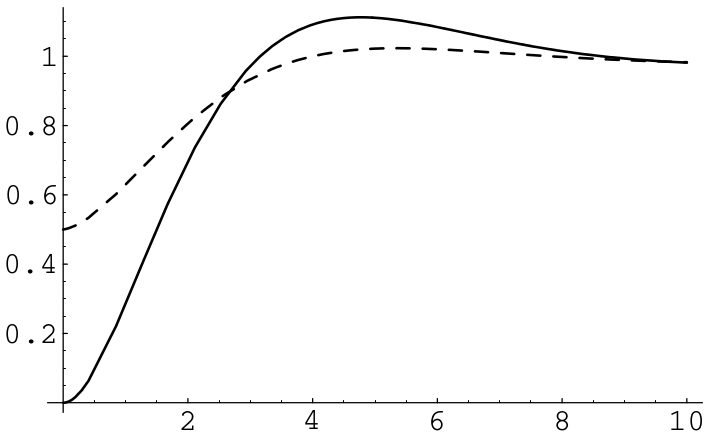
\includegraphics[width = .5\textwidth]{figs/Excess.png}
\end{center}
\vspace*{-.4cm}\hspace*{12cm}$\Delta t/\tau_S$
\captionof{figure}{Decay intensity $I(\Delta t)$ of $\phi\rightarrow \pi^+\pi^-\pi^+\pi^-$. The solid line is for $\zeta_{SL}=0$ and the dashed line for $\zeta_{SL}\neq 0$. \cite{Bernabeu:2006st} \label{FIG:Excess}}

\vspace*{.5cm}

The currently best 95\% C.L. limit on this parameter is set by KLOE with $\zeta_{SL} = 0.098$ \cite{Ambrosino2006315}.


\subsection{$\phi$ Production channels}

At LHCb, two $\phi$ production channels can be taken into consideration to do this study. One uses prompt $\phi$ coming directly from the primary vertex and the other uses $\phi$ from the decay $D_s^\pm \rightarrow \phi \pi^\pm$. Both production channels are illustrated in figure \ref{FIG:tracks}.
\vspace*{.5cm}
\begin{center}
\begin{minipage}{.49\textwidth}\centering
\begin{fmffile}{incl}
		\setlength{\unitlength}{.5mm}
		\fmfframe(0,0)(10,10){
		\begin{fmfgraph*}(75,65)
			\fmfleft{l1}
			\fmfright{r1,r2,r3,r4}
			\fmflabel{$\pi^+$}{r1}
			\fmflabel{$\pi^-$}{r2}					
			\fmflabel{$\pi^+$}{r3}
			\fmflabel{$\pi^-$}{r4}
			\fmf{plain}{r1,x1,r2}
			\fmf{plain}{r3,x2,r4}
			\fmf{dashes,label=$K^0$}{x1,y1}
			\fmf{dashes,label=$\overline{K}^0$}{y1,x2}
			\fmf{dashes,label=$\phi$}{l1,y1}
			\fmfforce{(.2w,.5h)}{y1}
		\end{fmfgraph*}}
\end{fmffile}
\end{minipage}
\begin{minipage}{.49\textwidth}\centering
\begin{fmffile}{Ds}
		\setlength{\unitlength}{.5mm}
		\fmfframe(0,0)(10,10){
		\begin{fmfgraph*}(75,65)
			\fmfleft{l1}
			\fmfright{r1,r2,r3,r4,r5}
			\fmflabel{$\pi^+$}{r1}
			\fmflabel{$\pi^-$}{r2}					
			\fmflabel{$\pi^+$}{r3}
			\fmflabel{$\pi^-$}{r4}
			\fmf{plain}{r1,x1,r2}
			\fmf{plain}{r3,x2,r4}
			\fmf{dashes,label=$K^0$}{x1,y1}
			\fmf{dashes,label=$\overline{K}^0$}{y1,x2}
			\fmf{dashes,label=$\phi$}{z1,y1}
			\fmf{plain}{l1,z1}
			\fmf{plain}{z1,r5}
			\fmflabel{$D_S^\pm$}{l1}
			\fmflabel{$\pi^\pm$}{r5}
		\end{fmfgraph*}}
\end{fmffile}
\end{minipage}
\captionof{figure}{Topology of prompt $\phi$ production (left) and $D_s^\pm \rightarrow \phi \pi^\pm$ (right) and the decay $\phi\rightarrow K^0 \overline{K}^0\rightarrow \pi^+\pi^-\pi^+\pi^-$. Solid lines indicate charged particles with tracks, dashed lines indicate neutral particles.} \label{FIG:tracks}
\end{center}

Including a cut on LHCb's geometric acceptance, the production cross sections for \SI{14}{TeV} as extrapolated from the \SI{7}{TeV} cross sections are for prompt $\phi$ \SI{3516}{\micro b} \cite{Aaij:2011uk} and for $D_s^\pm$ \SI{388}{\micro b} \cite{LHCb-CONF-2010-013}. Additionally, the branching fraction $\mathcal{B}(D_s^\pm \rightarrow \phi \pi^\pm) = (4.5 \pm 0.4)\%$ has to be taken into account for the production rate of $\phi$ in the $D_s^\pm$ channel. Both approaches are considered because the production rate of prompt $\phi$ is considerably higher than that of $\phi$ from $D_s^\pm$ decays, but $D_s^\pm \rightarrow \phi\pi^\pm$ might offer a better handle on background rejection because of the displaced $D_s^\pm$ vertex and a constraint on the $D_s^\pm$ mass.

\subsection{Background processes}

If one considers the excess of $\phi \rightarrow K^0 \overline{K}^0 \rightarrow \pi^+ \pi^- \pi^+ \pi^-$ for small $\Delta t$ due to CPT violation as signal, there are three main sources of background. One is the decay mode $\phi \rightarrow K_L K_S \rightarrow \pi^+\pi^-\pi^+\pi^-$ resulting from CP violation which from here one is going to be referred to as Standard Model (SM) background. Its decay intensity is plotted as the solid line in figure \ref{FIG:Excess}. The second background is so called regeneration background which results from the interaction of $K_L$ with matter and causes a transformation $K_L \rightarrow K_S$. The third background is combinatoric background of prompt kaons and pions.

\subsection{Track types}

In LHCb, different track types are defined depending on the sub-detectors in which the hits used to reconstruct the track are located. A schematic overview of the track types is given in figure \ref{FIG:tracktype}. For this study, we will consider only long tracks which are reconstructed with hits in the Velo (Vertex locator) and the other components of the tracking system, and downstream tracks which do not have hits in the Velo. Depending on its decay time a kaon can decay inside or outside the Velo and thus be reconstructed using two long pion tracks (LL) or two downstream pion tracks (DD). Kaons with long decay times are reconstructed using downstream tracks and kaons with short decay times are reconstructed using long tracks.


\begin{center}
    \def\svgwidth{.9\textwidth}
    \input{image.pdf_tex}
\captionof{figure}{Track types in LHCb: Upstream tracks are in the Velo and TT, downstream tracks in both outer trackers, and long tracks in all trackers. \cite{tracktypes}}\label{FIG:tracktype}
\end{center}

\section{Detector and processing efficiencies}
\label{SEC:Efficiencies}

\subsection{Dataset and selection}

To determine the number of events expected both for signal and background processes, Monte Carlo samples of prompt $\phi$ and $D_s^\pm \rightarrow \phi \pi^\pm$ have been used. These Monte Carlo files contain $1\cdot10^4$ events each. 

For the selection the stripping line \verb!PhiToKSKS! has been used. The version used in this study is not the final one. It can be found at \url{https://github.com/gdujany/phi2KsKs/blob/master/StrippingPhiToKSKS.py}. 

A summary of the cuts in the stripping line are given in table \ref{TAB:Stripping}.
\begin{center}

\resizebox{\textwidth}{!}{
\begin{tabular}{c|cc}
 & Prompt $\phi$ & $D_s^\pm \rightarrow \phi\pi^\pm$ \\ 
\hline 
$\pi$ from LL $K_S$ & TRGHOSTPROB $<$ 0.35 & TRGHOSTPROB $<$ 0.35\\
& P $>$ 2\,GeV & P $>$ 2\,GeV \\
& MIPCHI2DV(PRIMARY) $>$ 9& MIPCHI2DV(PRIMARY) $>$ 9\\
\hline 
$\pi$ from DD $K_S$ & P $>$ 2\,GeV & P $>$ 2\,GeV \\
& MIPCHI2DV(PRIMARY) $>$ 4& MIPCHI2DV(PRIMARY) $>$ 4\\
\hline 
$K_S$ &ADOCACHI2CUT(25, '')&ADOCACHI2CUT(25, '')\\
&VFASPF(VCHI2) $<$ 25&VFASPF(VCHI2) $<$ 25\\
&PT $>$ 500\,MeV&PT $>$ 500\,MeV\\
&ADMASS('KS0') $<$ 20\,MeV&ADMASS('KS0') $<$ 20\,MeV\\
&BPVVD $>$ 10\,mm&BPVVD $>$ 10\,mm\\
&BPVVDCHI2 $>$ 50&BPVVDCHI2 $>$ 50\\
&VFASPF(VCHI2PDOF) $<$ 10 &VFASPF(VCHI2PDOF) $<$ 10\\
&BPVDIRA $>$ 0.9999&BPVDIRA $>$ 0.9999\\
\hline
$\phi$ & LL LL or LL DD combinations & LL LL or LL DD combinations\\
&APT $>$ 1000\,MeV & APT $>$ 1000\,MeV\\
&AM $<$ 1100\,MeV & AM $<$ 1100\,MeV\\
&ACUTDOCACHI2(100,'') & ACUTDOCACHI2(100,'')\\ 
&M $<$ 1070\,MeV & M $<$ 1090\,MeV\\
&VFASPF(VCHI2/VDOF) $<$ 10 & VFASPF(VCHI2/VDOF) $<$ 10\\
&MIPCHI2DV(PRIMARY) $<$ 100 & MIPCHI2DV(PRIMARY) $<$ 100\\
\hline
$\pi$ from $D_s$ &&PT $>$ 250\,MeV\\
&&MIPCHI2DV(PRIMARY) $>$ 4\\
&&MIPCHI2DV(PRIMARY) $<$ 300\\
&&TRGHOSTPROB $<$ 0.35\\
\hline
$D_s$ &&APT $>$ 800\,MeV\\
&&ADAMASS(1920\,MeV) $<$ 130\,MeV\\
&&ACUTDOCACHI2(100,'')\\
&&DMASS(1920\,MeV) $<$ 100\,MeV\\
&&VFASPF(VCHI2/VDOF) $<$ 10\\
&&MIPCHI2DV(PRIMARY) $<$ 100\\
\hline
Post-stripping cuts & $\SI{1010}{MeV}<$phi\_M$<\SI{1030}{MeV}$ &$\SI{1010}{MeV}<$phi\_M$<\SI{1030}{MeV}$\\
&&\SI{1955}{MeV}$<$Ds\_M$<$\SI{1985}{MeV}\\
&&IPCHI2 $\geq$ 15
\end{tabular} }
\captionof{table}{Summary of all cuts done in the stripping line and in post-stripping selection, both for prompt $\phi$ and $D_s^\pm\rightarrow\phi\pi^\pm$.}\label{TAB:Stripping}
\end{center}
The mass windows used for all following studies are $\SI{1010}{MeV} < m(\phi) < \SI{1030}{MeV}$ and $\SI{1955}{MeV} < m(D_s^\pm) < \SI{1985}{MeV}$. In order to reject prompt $\phi$, in the $D_s^\pm \rightarrow \phi \pi^\pm$ selection the cut $\chi^2 \geq 15$ on the $\chi^2$ of a fit matching the $\phi$ origin vertex to the primary vertex was added. 


\begin{center}
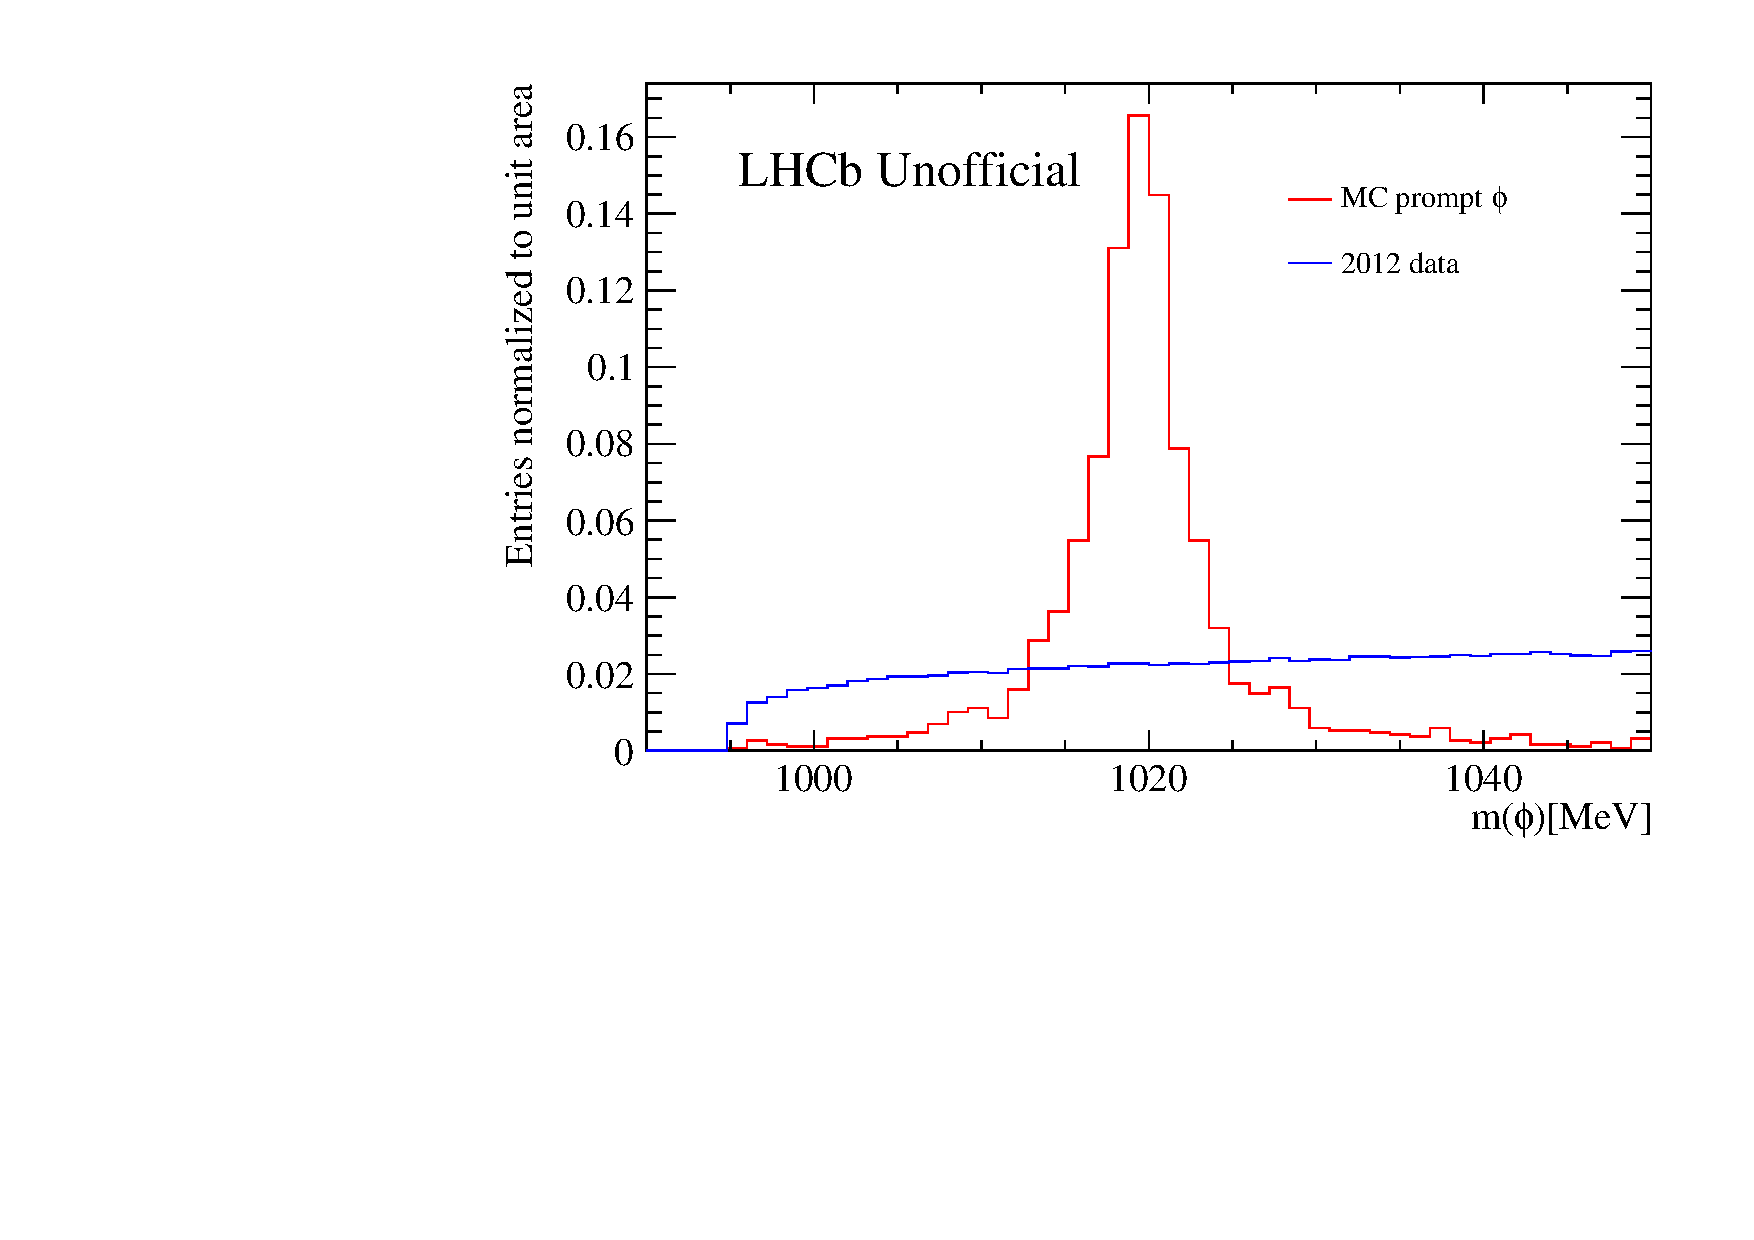
\includegraphics[height = .49\textwidth]{/home/soonja/lxplus/phi2KsKs/phi2KsKs/preliminaryStudies/m_phi_incl.pdf}
\captionof{figure}{Invariant mass of $\phi$ after applying the selection. The Monte Carlo shows the spectrum for $\phi\rightarrow K_SK_S\rightarrow \pi^+\pi^-\pi^+\pi^-$ whereas the 2012 data contains mostly background events.}\label{FIG:IM1}
\end{center}

\begin{center}
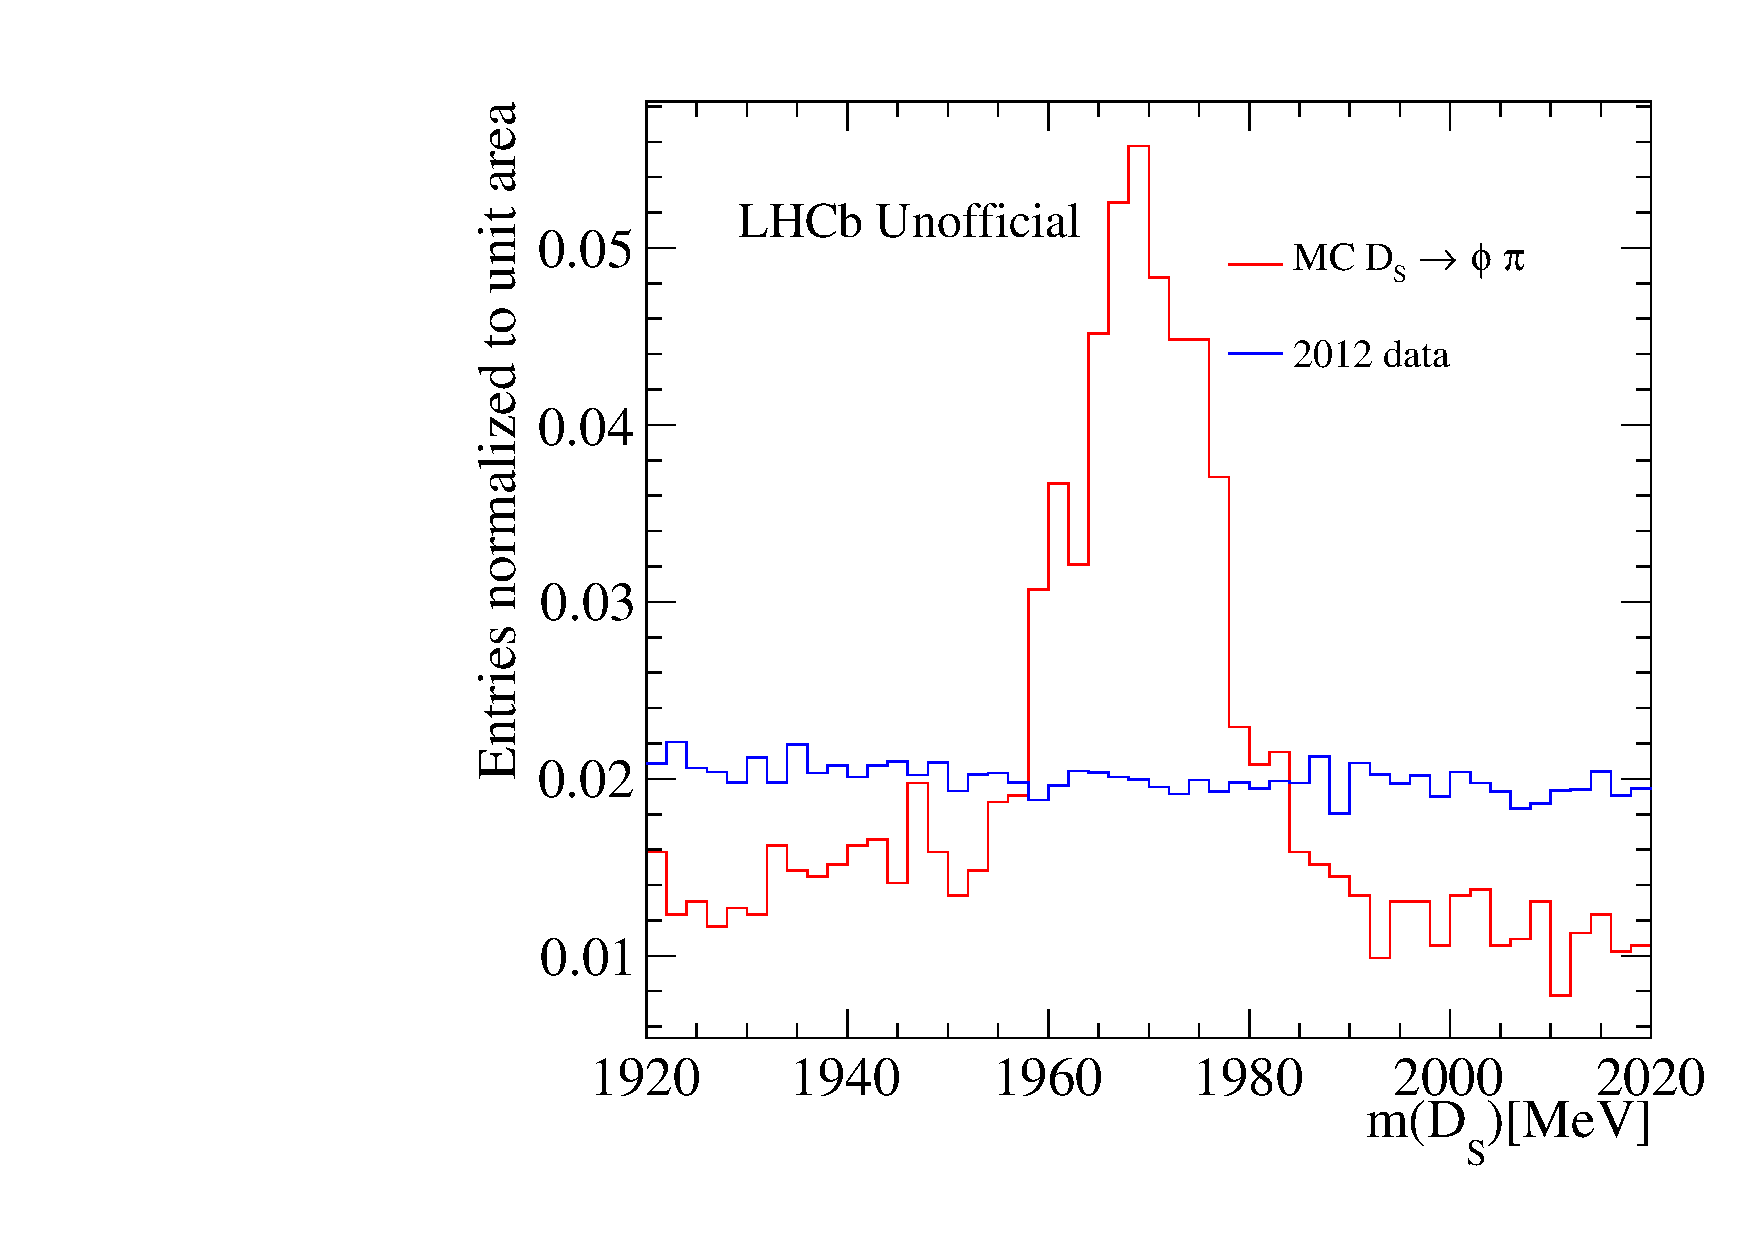
\includegraphics[width = .49\textwidth]{/home/soonja/lxplus/phi2KsKs/phi2KsKs/preliminaryStudies/m_Ds_Ds.pdf}
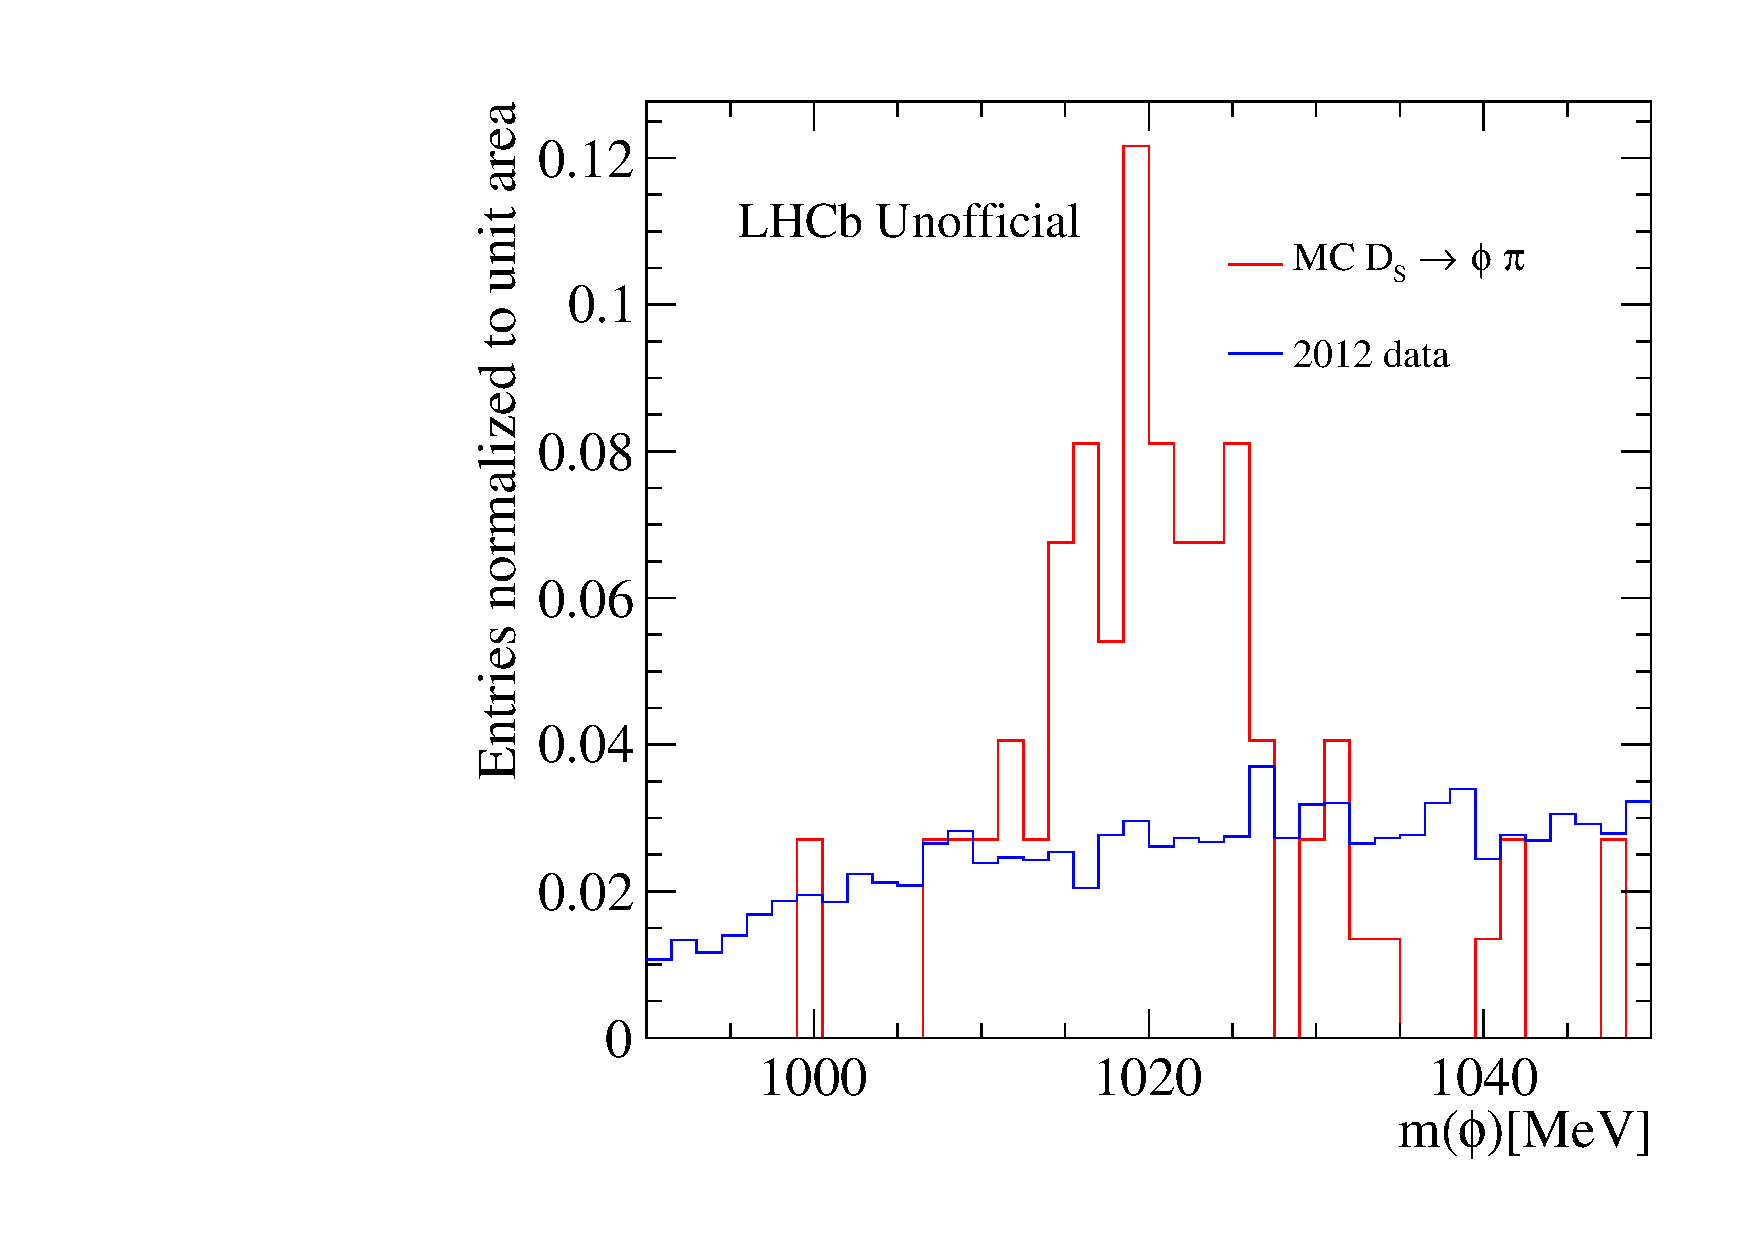
\includegraphics[width = .49\textwidth]{/home/soonja/lxplus/phi2KsKs/phi2KsKs/preliminaryStudies/m_phi_Ds.pdf}
\captionof{figure}{Invariant mass of $D_s$ and $\phi$ after applying the selection. The Monte Carlo shows the spectra for $D_s^\pm \rightarrow \phi\pi^\pm\rightarrow K_SK_S\rightarrow \pi^+\pi^-\pi^+\pi^-\pi^\pm$ whereas the 2012 data contains mostly background events.}\label{FIG:IM2}
\end{center}


Additional to the signal Monte Carlo samples, the 2012 data set was processed with the selection. For the prompt $\phi$ selection, the \verb!CHARM.mDST! container was used, as was the \verb!CHARMCOMPLETEEVENT.DST! container for the $D_s^\pm \rightarrow \phi \pi^\pm$ selection (both are \verb!Reco14!). The resulting spectra of the invariant masses of $\phi$ and $D_s^\pm$ normalized to unit area can be found in figures \ref{FIG:IM1} and \ref{FIG:IM2}.


\subsection{Efficiencies}
From the Monte Carlo, reconstruction and trigger efficiencies have been determined. The probabilities of the kaon decays have been determined using the decay intensities in equation \eqref{EQ:DI1} and \eqref{EQ:DI2}, with 
$\zeta_{SL}$ set to 0.098, the 95\% C.L. limit set by KLOE. It is estimated that to decay, on 
average, inside the beampipe, the decay time of the kaons has to be less than 25\,ps, and to be reconstructed at all, the decay time has to be less than 200\,ps. The estimate for the background yield is the number of events in the 2012 data after applying the selection. All resulting values can be found in table \ref{TAB:Efficiencies}.


\begin{center}
\resizebox{\textwidth}{!}{
\begin{tabular}{ccc}
&Prompt $\phi$ & $D_s \rightarrow \phi \pi$ \\
\hline 
\hline
\vspace*{-6pt}\\
Cross section (\SI{14}{TeV}), LHCb acceptance &\SI{ 3516 }{\micro\barn} & \SI{ 388 }{\micro\barn} \\
\hline
Branching fractions & 34.2\% & 4.5\% $\cdot$  34.2\% \\
\hline
Fiducial cuts efficiency & 2.5\% & 7.0\%\\
\hline
Probability $K_sK_s \rightarrow 4\pi$, \\
 exactly 1 (2) decays inside beampipe &\multicolumn{2}{c}{$ 15.1\%$ ( $2.8\%$ )} \\
\hline
Probability $K_sK_L \rightarrow 4\pi$ (CPV),\\
exactly 1 (2) decays inside beampipe &\multicolumn{2}{c}{$ 3.98\cdot 10^{-7}$ ( $4.99\cdot 10^{-10}$ )} \\
\hline
Upper limit KLOE probability\\ $K_sK_L \rightarrow 4\pi$ (CPV 
+ CPTV),\\ exactly 1 (2) decays inside beampipe &\multicolumn{2}{c}{$  5.13\cdot 10^{-7}$ ( $1.64\cdot 10^{-8}$ )}\\
\hline
Reconstruction \& selection efficiency &  7.9\% ( 7.6\% )  & 1.4\% ( 3.9\% )\\
L0 efficiency&  16.1\% ( 18.6\% )&  23.0\% ( 19.5\% )\\
HLT1 efficiency&  13.7\% ( 16.7\% )& 35.6\% ( 25.0\% )\\
HLT2 efficiency&  65.6\% ( 100.0\% )& 68.8\% ( 100.0\% )\\
\hline
Total efficiency &$ 4.39\cdot 10^{-5} $ ( $ 5.85\cdot 10^{-5} $ )&$ 8.18\cdot 10^{-5} $ ( $ 1.32\cdot 10^{-4} $ )\\
Expected events SM background / fb$^{-1}$ &$ 21 $ ( $ 3.51\cdot 10^{-2} $)&$ 1.94\cdot 10^{-1} $ ( $ 3.94\cdot 10^{-4} $)\\
Upper limit for SM background + signal (KLOE)  / fb$^{-1}$ &$ 27 $ ( $ 1.15 $ )&$ 2.5\cdot 10^{-1} $ ( $ 1.29\cdot 10^{-2} $ )\\
Combinatoric background (data 2012) / fb$^{-1}$ & 163110 ( 29120 ) &  450 ( 2030 )\\
\end{tabular}
}
\captionof{table}{Cross sections, branching fractions, efficiencies and resulting event yields for signal, standard model background, and combinatoric background. If two numbers are given, the one in brackets assumes two kaons decaying inside the beampipe, whereas for the other it is required that exactly one of the two kaons decays inside the beampipe.}\label{TAB:Efficiencies}
\end{center}

From the event yield one can conclude that the signal to background ratio is in the same order of magnitude for both approaches and not much is gained from using the $D_s^\pm \rightarrow \phi \pi^\pm$ approach.
\section{Background studies with minimum bias Monte Carlo}

In order to better understand the combinatoric background, minimum bias Monte Carlo files\footnote{The files can be found in the LHCb bookkeeping under the references \texttt{/MC/2012/30000000/Beam4000GeV-2012-MagUp-Nu2.5-Pythia8/Sim08a/Digi13/Trig0x409f0045/\\Reco14a/Stripping20NoPrescalingFlagged/ALLSTREAMS.DST},\\\texttt{/MC/2012/30000000/Beam4000GeV-2012-MagDown-Nu2.5-Pythia8/Sim08a/Digi13/Trig0x409f0045/\\Reco14a/Stripping20NoPrescalingFlagged/ALLSTREAMS.DST},\\\texttt{/MC/2012/30000000/Beam4000GeV-2012-MagUp-Nu2.5-Pythia8/Sim08c/Digi13/Trig0x409f0045/\\Reco14a/Stripping20NoPrescalingFlagged/ALLSTREAMS.DST}, and \\\texttt{/MC/2012/30000000/Beam4000GeV-2012-MagDown-Nu2.5-Pythia8/Sim08c/Digi13/Trig0x409f0045/\\Reco14a/Stripping20NoPrescalingFlagged/ALLSTREAMS.DST}.} have been processes with the same selections as described in section \ref{SEC:Efficiencies}.  From the 42 million input events, those that remain after the selection have the following background categories:
\begin{center}
\begin{tabular}{c|c|c}
Background category & Prompt $\phi$ & $D_s \rightarrow \phi \pi$ \\ 
\hline 
light flavour & 17(17) & 0 \\ 
$b\overline{b}$ & 1(1) & 0 \\ 
different PV & 3(2) & 0 \\ 
physical bkg, partl. reconstructed & 1(1) & 1(1) \\ 
ghosts & 0 & 1(0) \\ 
\hline 
total & 21(20) & 2(1) \\  
\end{tabular} 
\captionof{table}{Background categories of the minimum bias Monte Carlo events remaining after the selection. The number in brackets is the number of background events with true $K_S$.}
\end{center}

It can be concluded that 80\% of the background after the prompt $\phi$ selection is prompt $K_S$ originating from the primary vertex. For the $D_s^\pm \rightarrow \phi\pi^\pm$ selection, the number of events in the Monte Carlo sample is too low to gain more information about the background types.

\section{Time resolution}
Since CPT violation would be visible as an excess of $\phi \rightarrow K^0 \overline{K}^0 \rightarrow \pi^+ \pi^- \pi^+ \pi^-$ for small $\Delta t$, knowledge about the time resolution of the detector for this system is important.
Two differenent methods have been considered for the reconstruction of the decay times. 
The first uses the DaVinci class TupleToolPropertime %\footnote{\url{http://lhcb-release-area.web.cern.ch/LHCb-release-area/DOC/rec/releases/v14r2/doxygen/d3/df5/class_tuple_tool_propertime.html}} 
to determine the decay times from the reconstructed particles. The standard reconstruction follows a bottom-up approach, starting with parameters of the reconstructed final state particles and then working its way up by determining the parameters of each mother particle via a fit to those parameters of its daughter particles \cite{2005NIMPA.552..566H}.
The second method uses the DecayTreeFitter %\footnote{\url{https://lhcb-release-area.web.cern.ch/LHCb-release-area/DOC/hlt/latest_doxygen/df/d04/namespace_decay_tree_fitter.html}}.
which performs a simultaneous fit of all vertices \cite{2005NIMPA.552..566H}. For this study, in this fit, the kaon mass was constrained to the nominal $K_S$ mass.


To determine the resolution, the reconstructed decay times $t(\text{reconstructed})$ were compared with the true decay times $t(\text{true})$ for the $D_S^\pm \rightarrow \phi \pi^\pm$ and the prompt $\phi$ Monte Carlo, the different figures being presented next to each other in the following.


\subsection{Using the DecayTreeFitter}
The DecayTreeFitter does not allow for negative decay times. Therefore 
\begin{equation}
t(\text{reconstructed})-t(\text{true})\geq - t(\text{true}),
\end{equation}
which leads to a sharp edge for negative residuals as illustrated for LL kaons in figure \ref{FIG:LL-DTF}. 

The resolution was estimated by fitting the residual for those cases where $t(\text{reconstructed})-t(\text{true}) \geq 0$ to a Breit Wigner distribution
\begin{equation}
N(\delta t) = \frac{a}{(\delta t- \mu)^2 - \Gamma^2/4}, \qquad \delta t = t(\text{reconstructed})-t(\text{true}) \label{EQ:BWt}
\end{equation}
as shown in figure \ref{FIG:timeres-LL-DTF}. For this specific fit, the centre was fixed to $\mu =0$.

\begin{center}
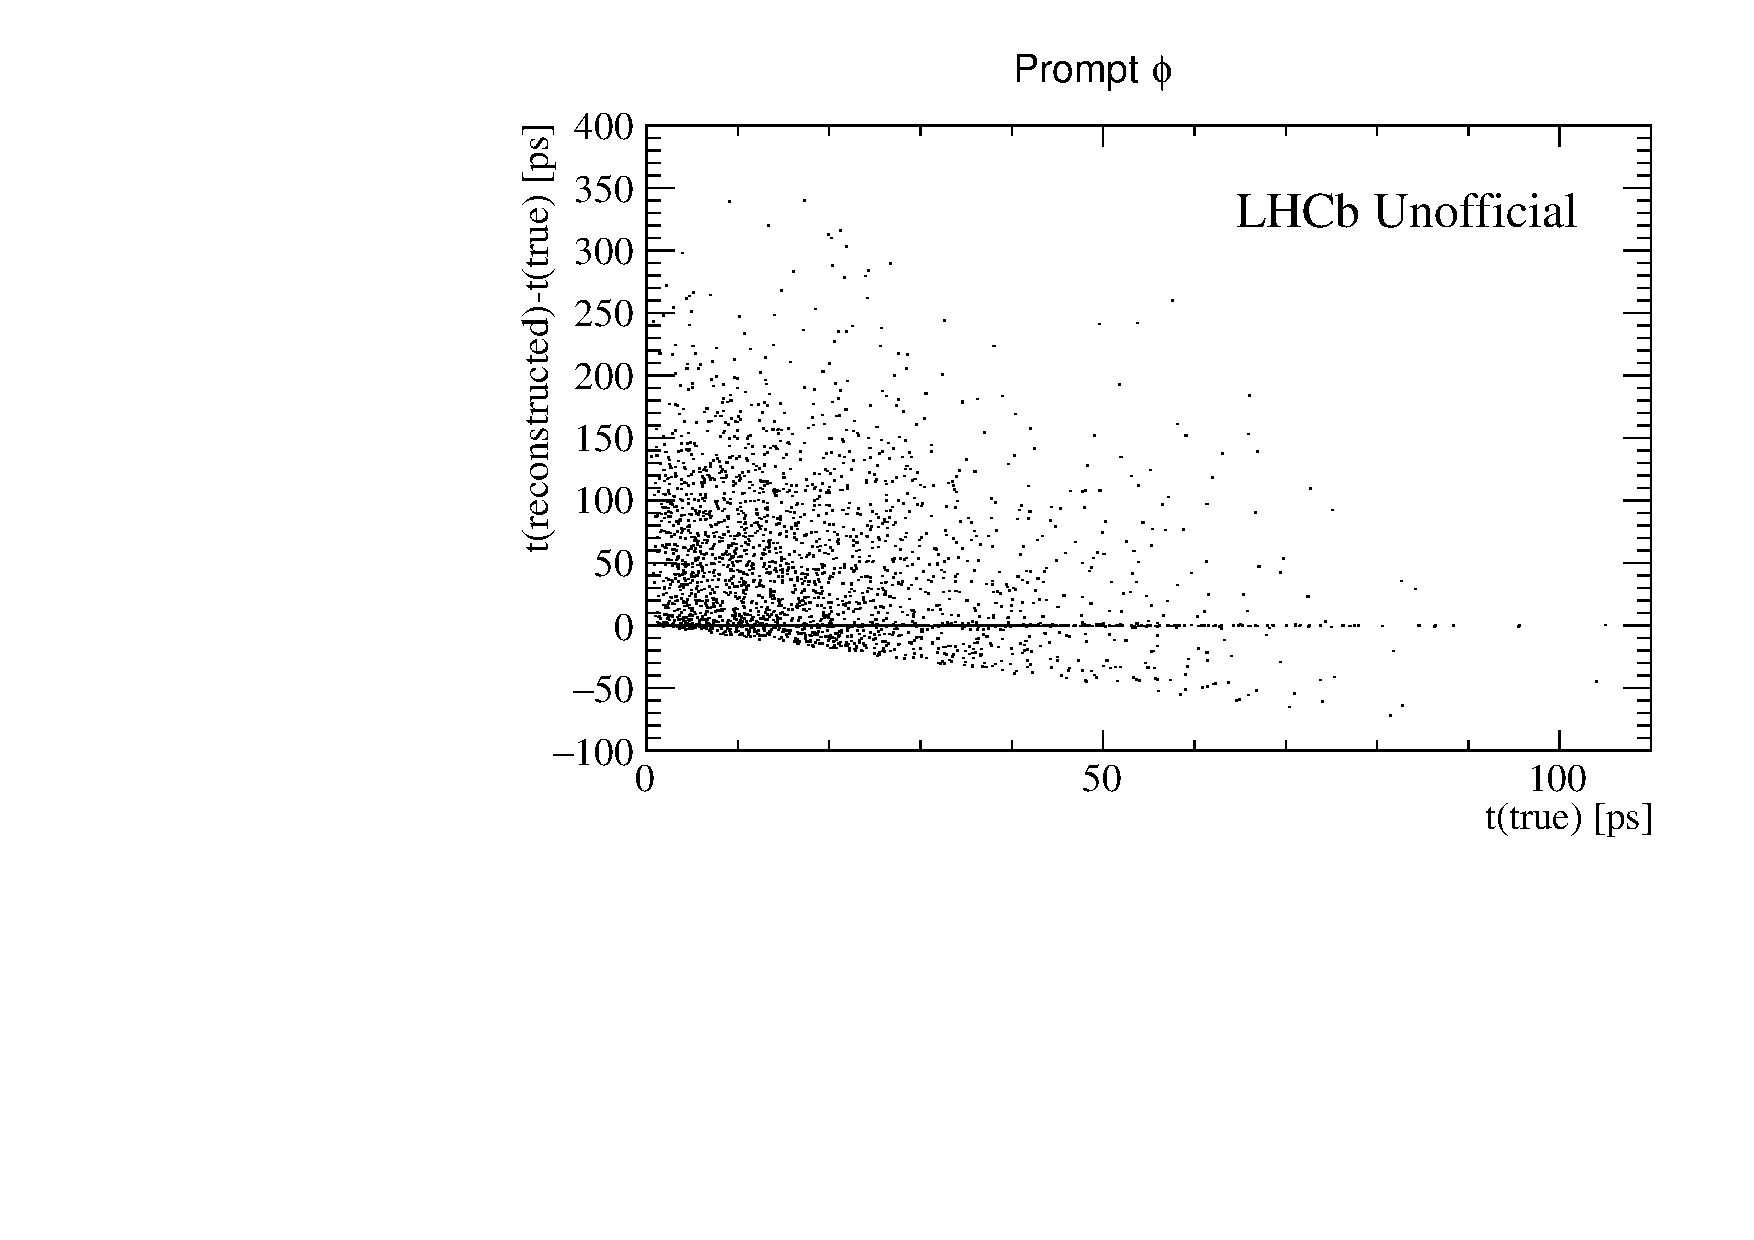
\includegraphics[width=.49\textwidth]{figs/time_res_incl/LL-DTF.pdf}
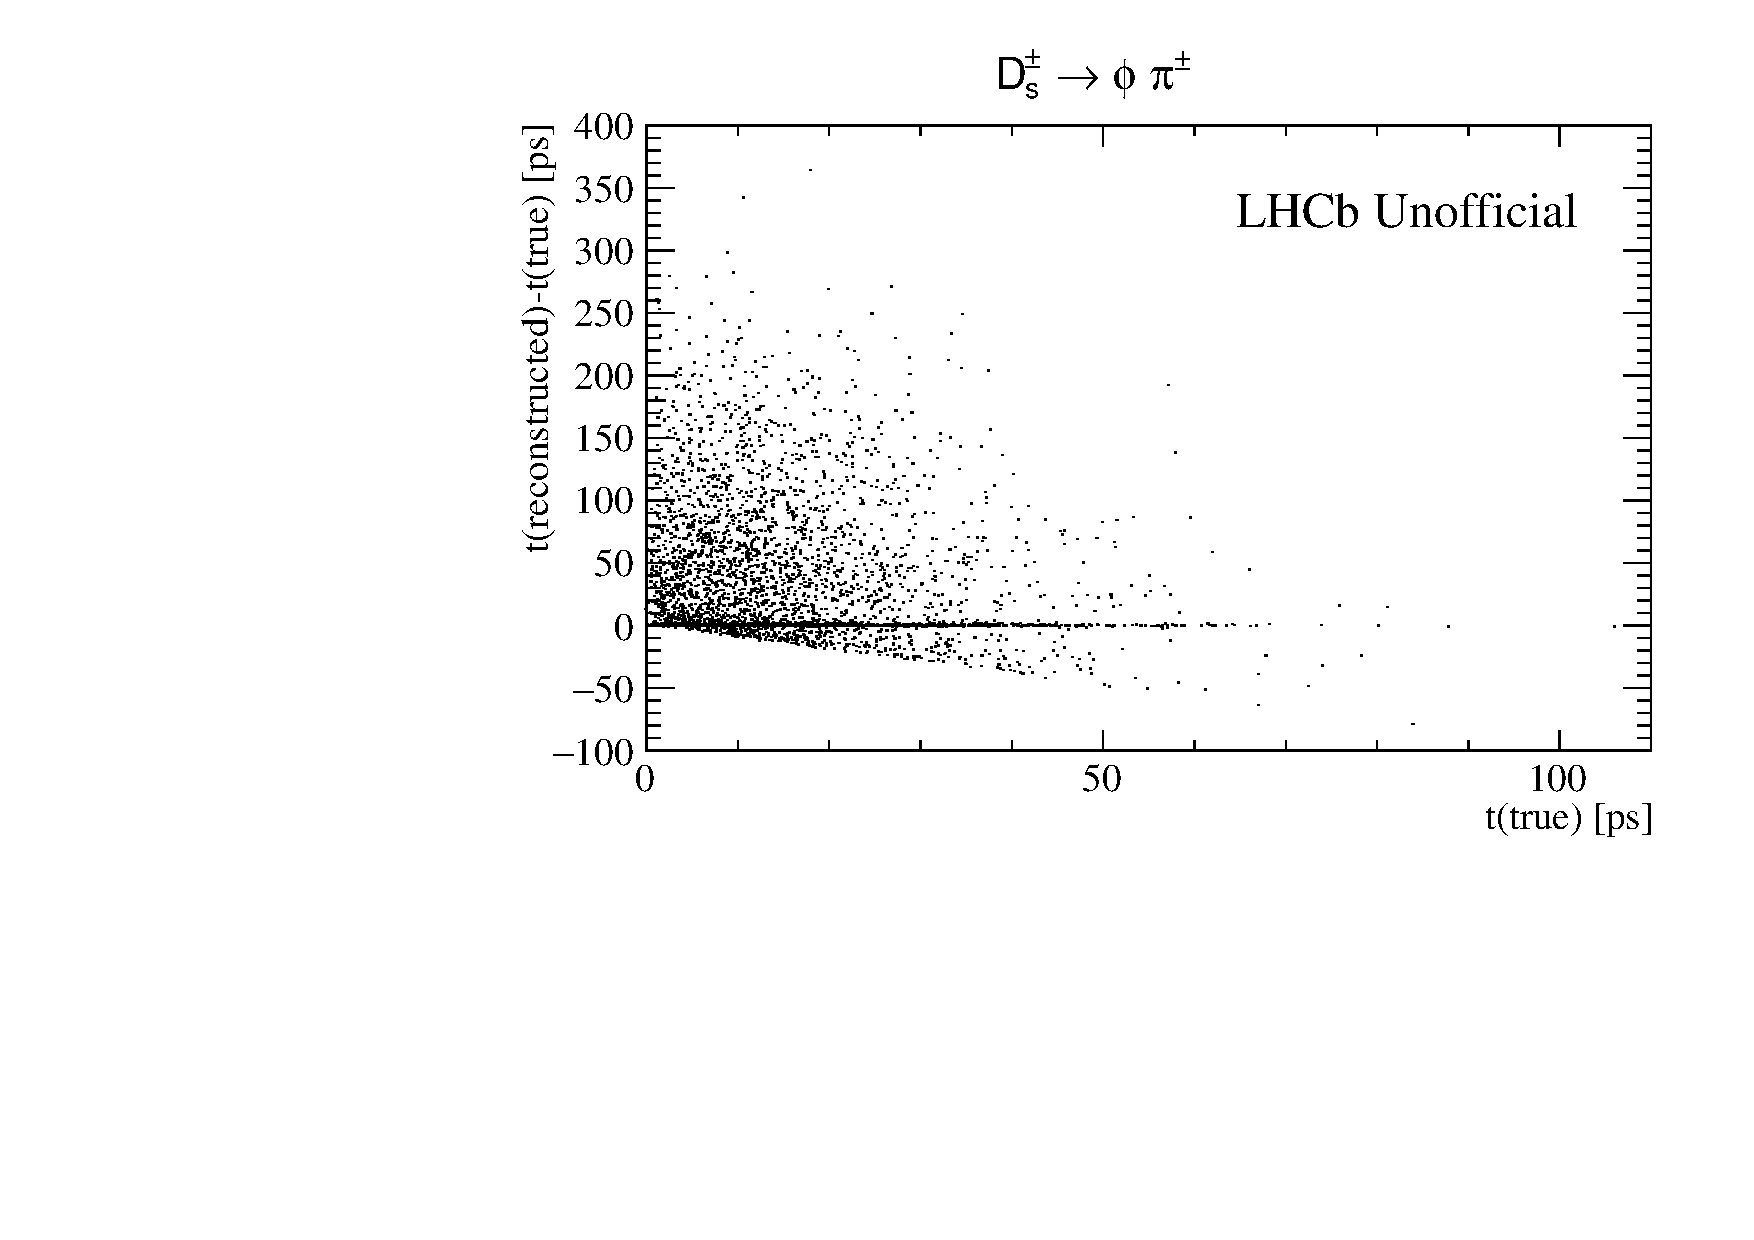
\includegraphics[width=.49\textwidth]{figs/time_res_Ds/LL-DTF.pdf}
\captionof{figure}{Residual of $t$ for LL kaons reconstructed via DecayTreeFitter plotted against the true value of $t$. }\label{FIG:LL-DTF}


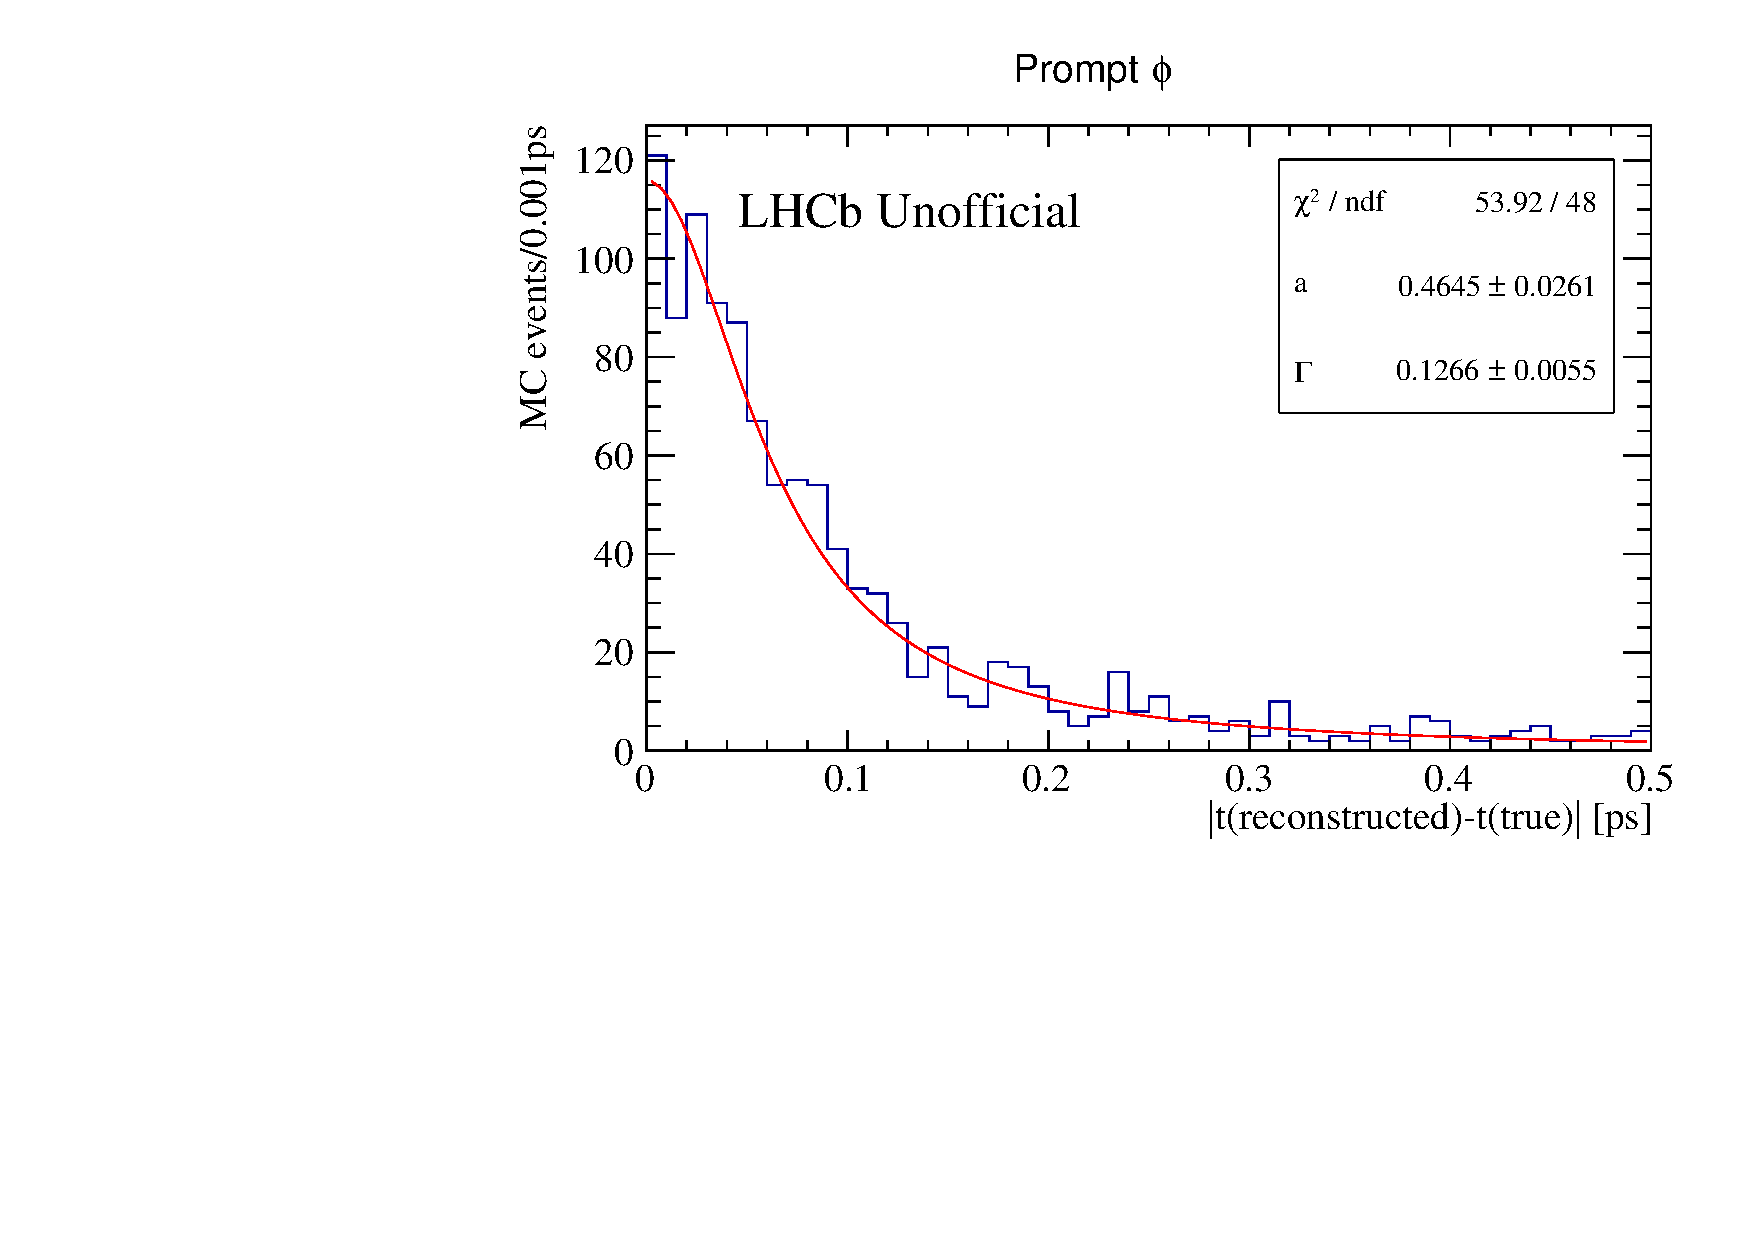
\includegraphics[width=.49\textwidth]{figs/time_res_incl/timeResolution-LL-DTF.pdf}
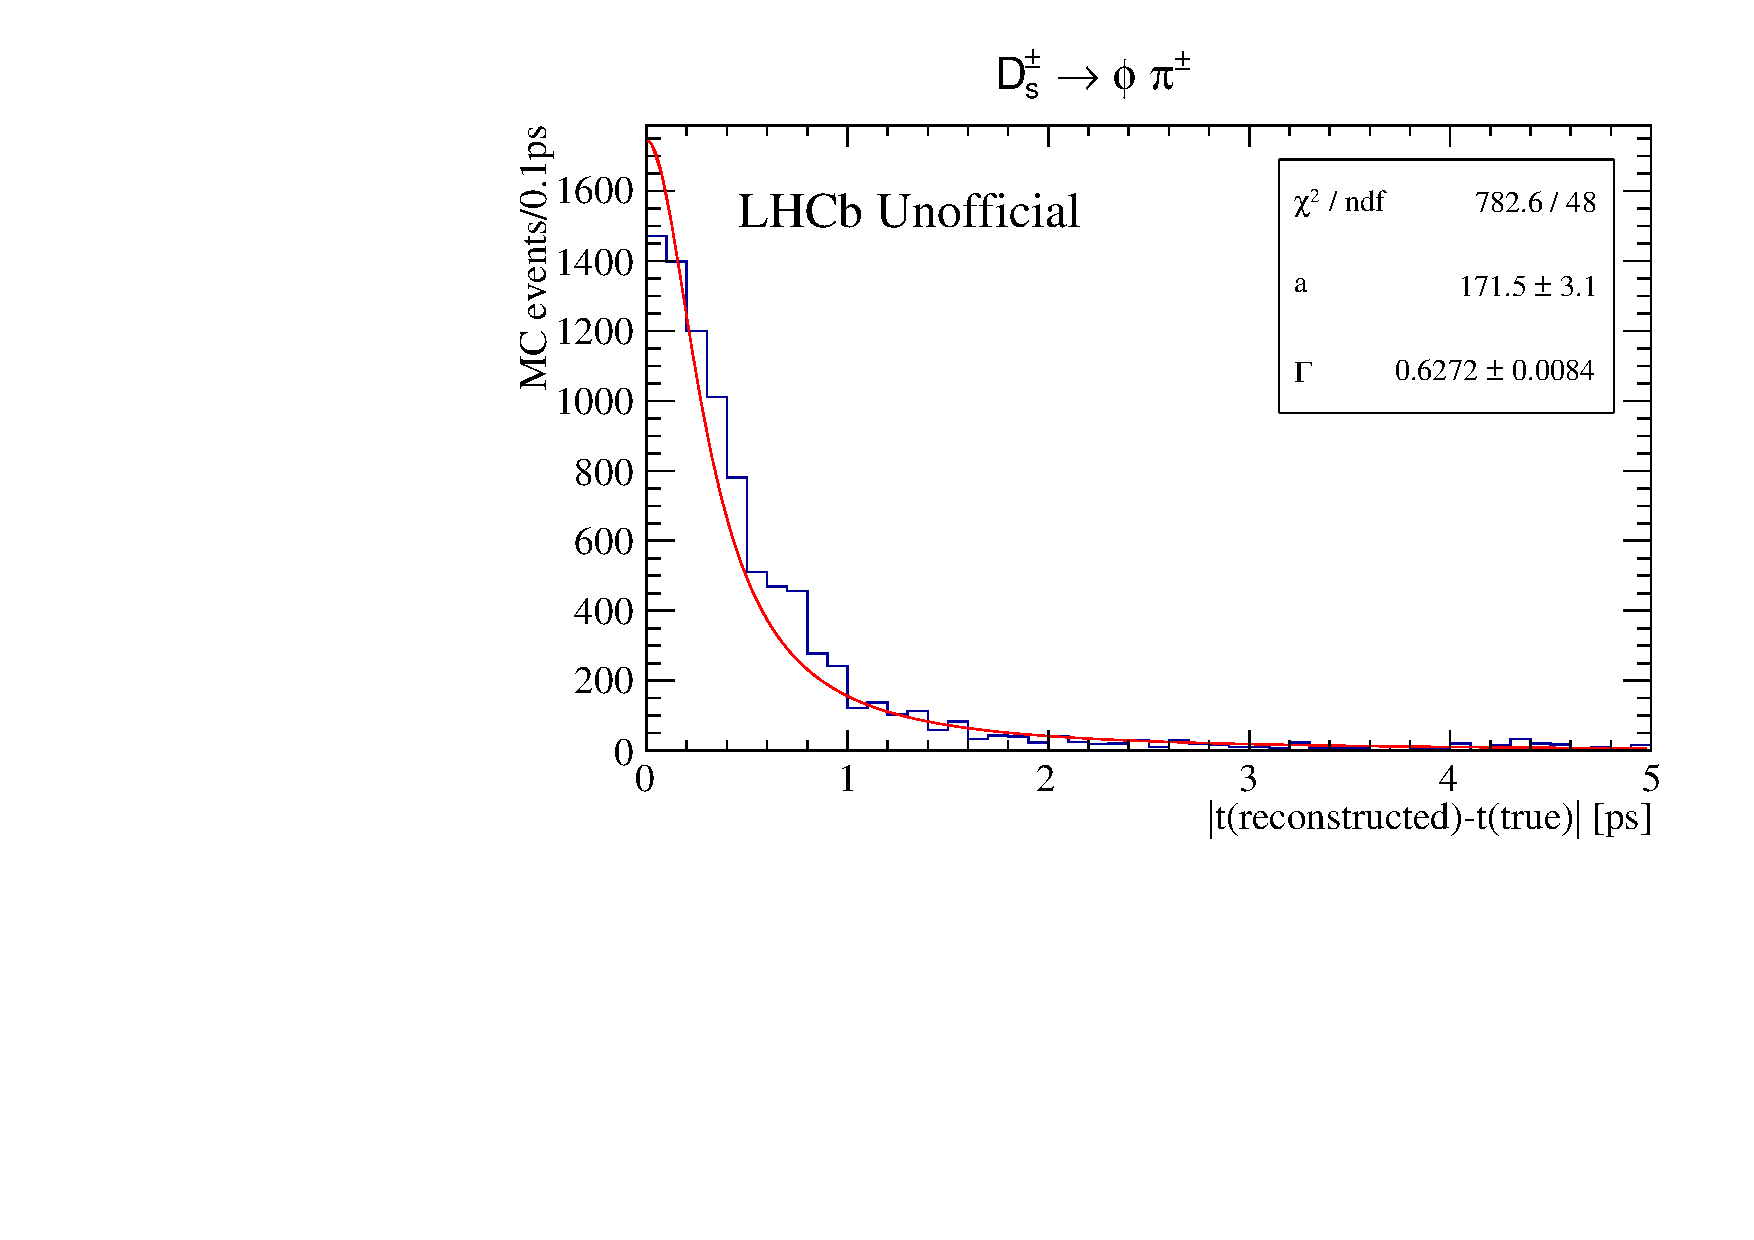
\includegraphics[width=.49\textwidth]{figs/time_res_Ds/timeResolution-LL-DTF.pdf}
\captionof{figure}{Resolution of LL kaon decay times $t$ reconstructed via the DecayTreeFitter. }\label{FIG:timeres-LL-DTF}


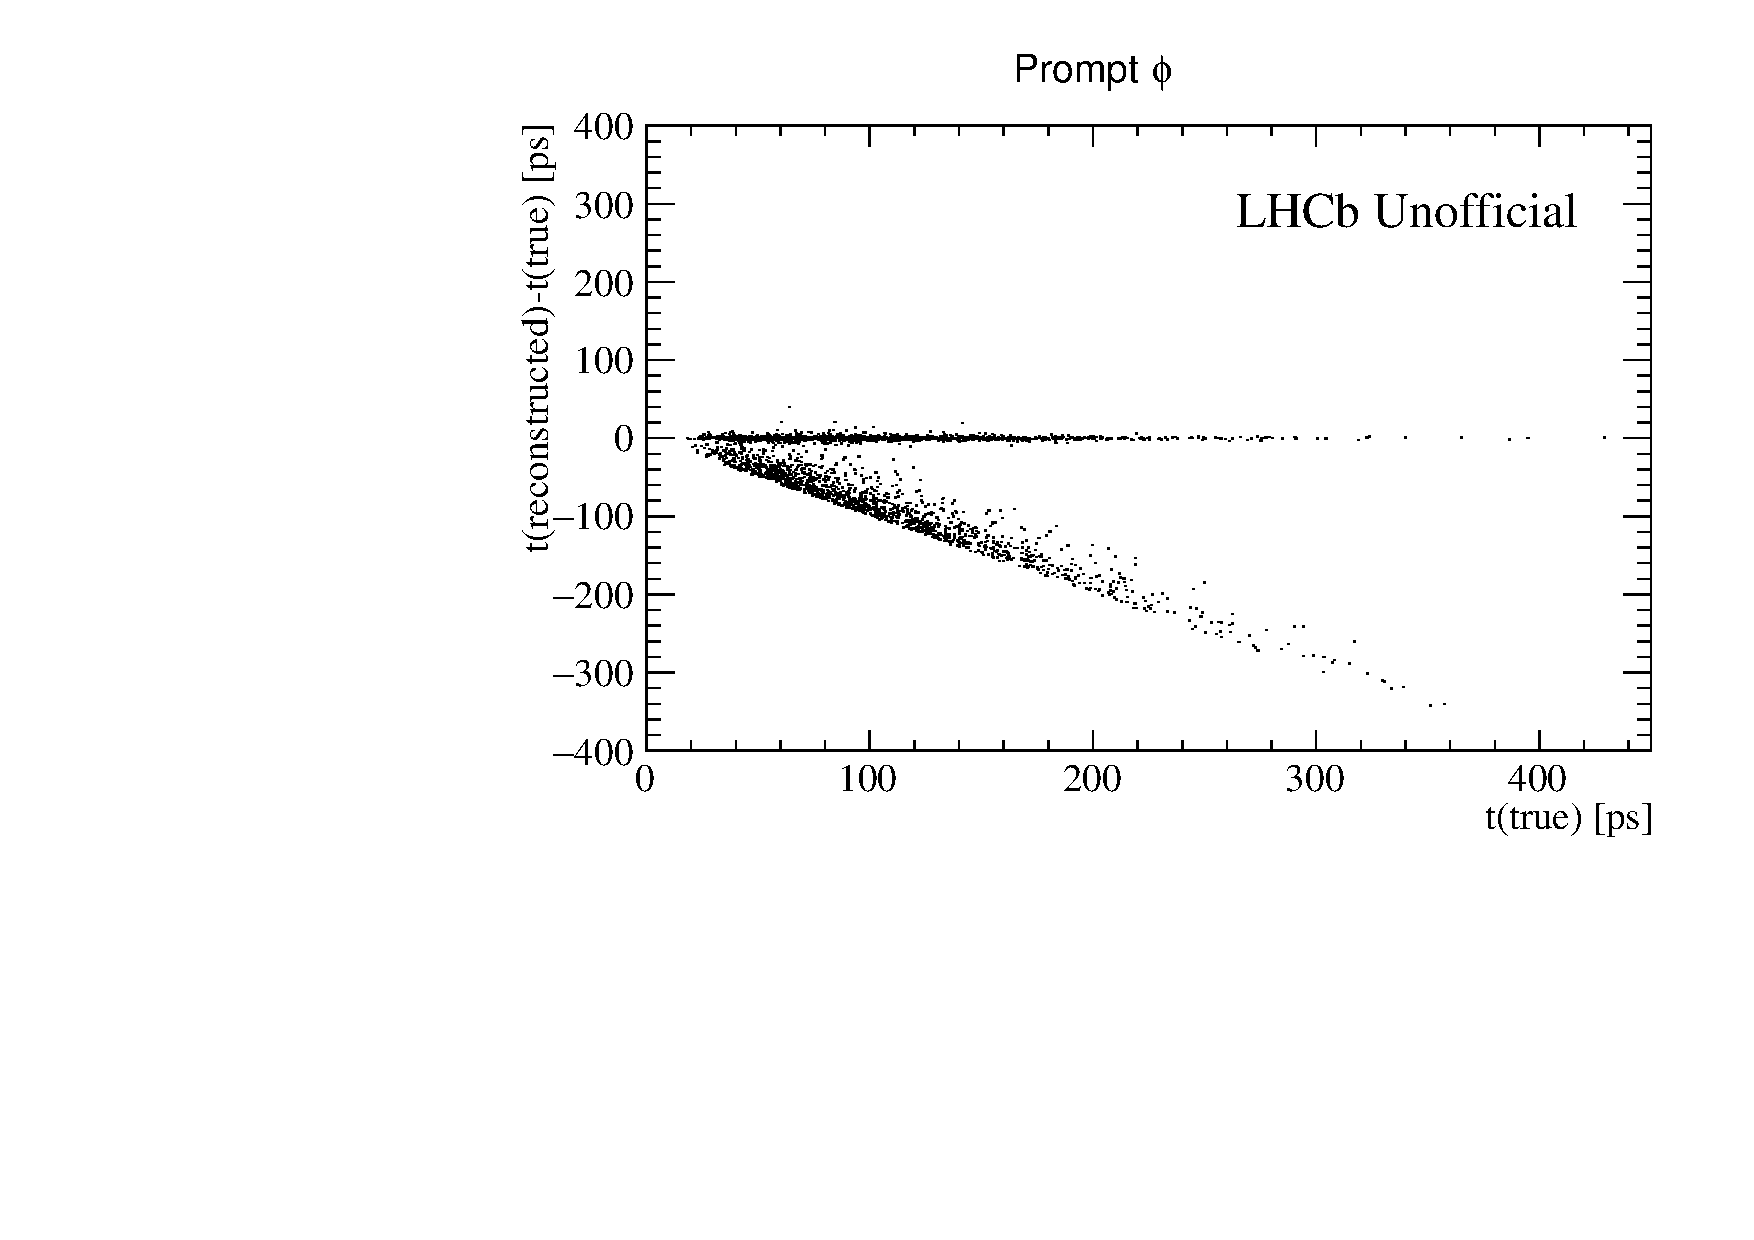
\includegraphics[width=.49\textwidth]{figs/time_res_incl/DD-DTF.pdf}
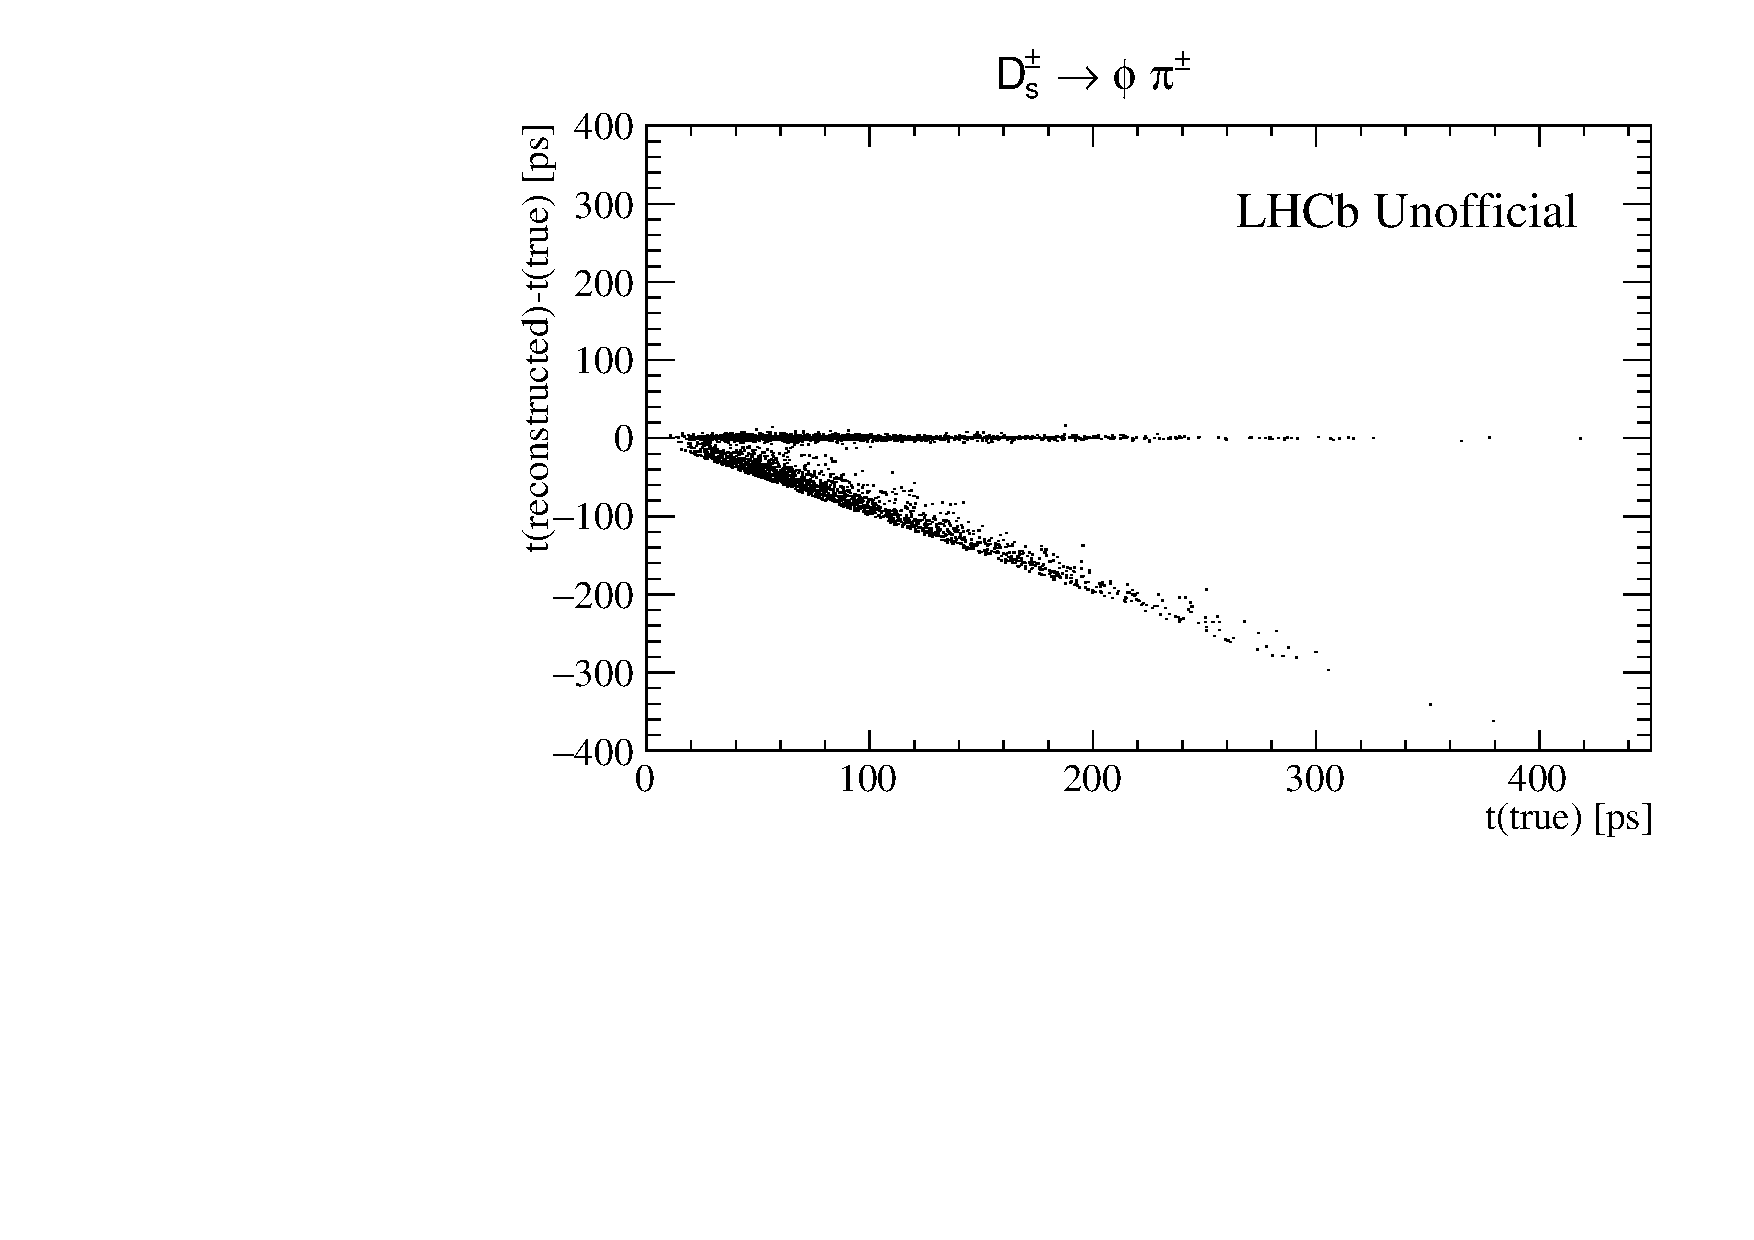
\includegraphics[width=.49\textwidth]{figs/time_res_Ds/DD-DTF.pdf}
\captionof{figure}{Residual of $t$ for DD kaons reconstructed via DecayTreeFitter plotted against the true value of $t$. }\label{FIG:DD-DTF}

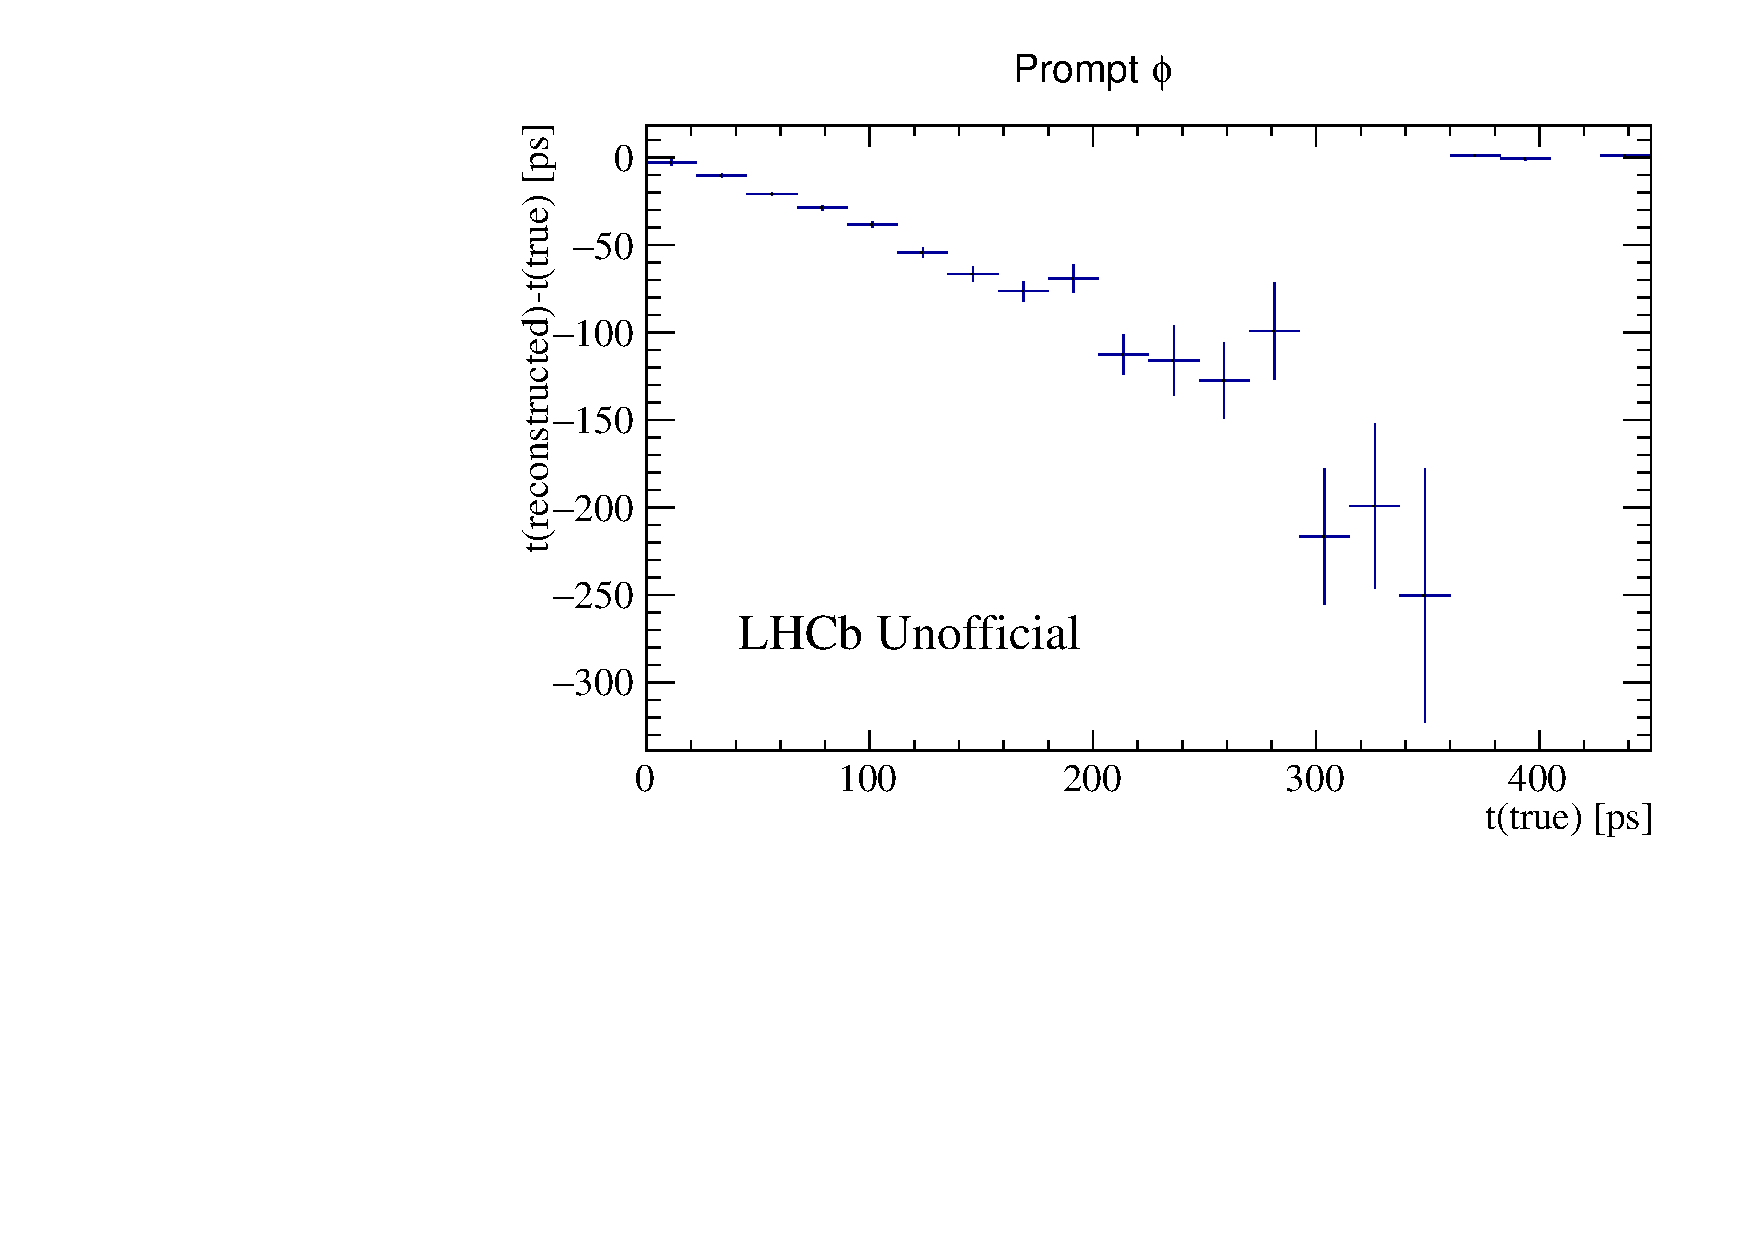
\includegraphics[width=.49\textwidth]{figs/time_res_incl/DD-DTF-prof.pdf}
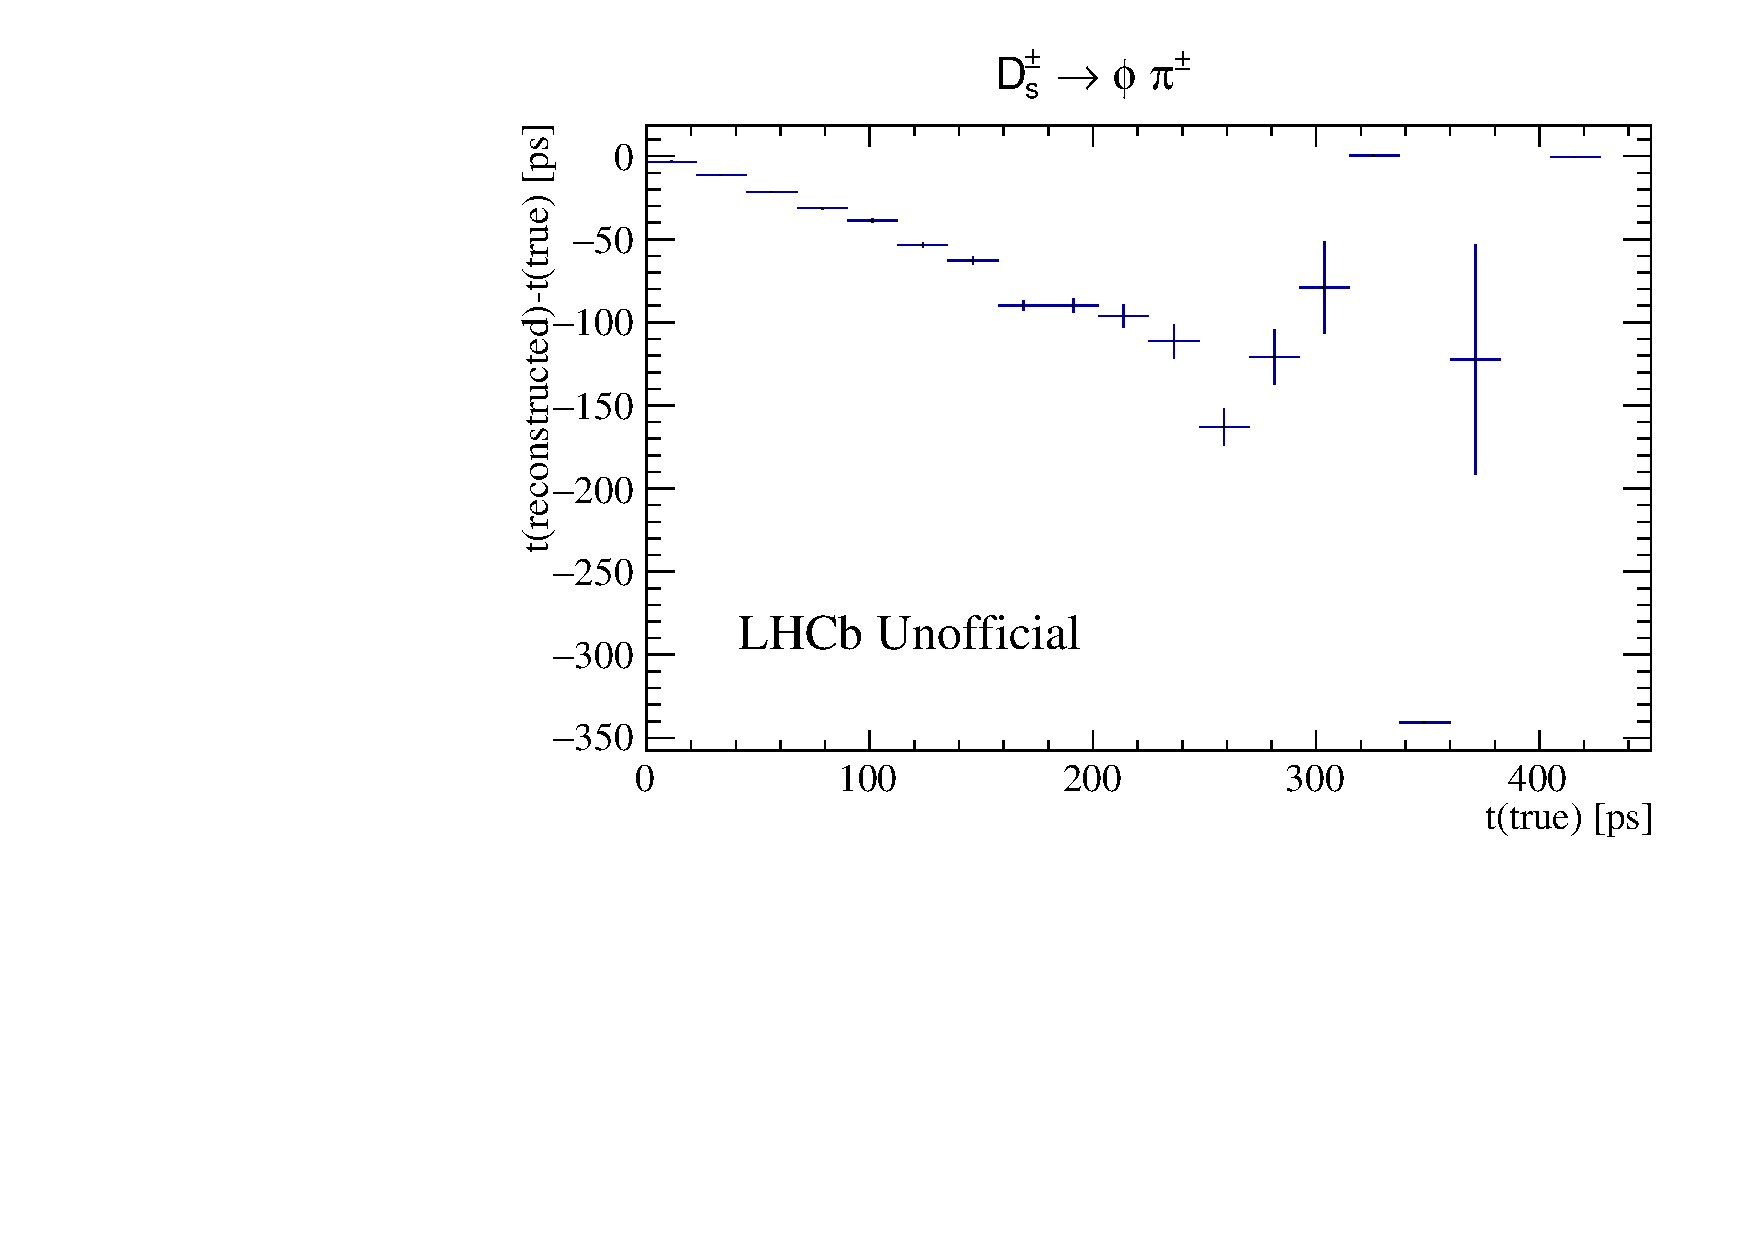
\includegraphics[width=.49\textwidth]{figs/time_res_Ds/DD-DTF-prof.pdf}
\captionof{figure}{Average residual of $t$ for DD kaons reconstructed via DecayTreeFitter plotted against the true value of $t$. }\label{FIG:DD-DTF-prof}
\end{center}


For DD kaons, sensitivity on the decay times is not given because the DecayTreeFitter sometimes reconstructs the decay times of the kaons as close to zero, maybe due to a lack of information available, which can be seen in figure \ref{FIG:DD-DTF}. This results in an underestimation of the decay times as shown in figure \ref{FIG:DD-DTF-prof}.
Therefore it is not advised to use the DecayTreeFitter in the context of decay time reconstruction with downstream tracks.

Since for probing the CPT invariance of the system, the observable $\Delta t = |t_1 - t_2|$ is used, its resolution for LL kaons has been studied as well, as it is displayed in figure \ref{FIG:timres-LL-DTF-prof}. To do this, the residual $\delta(\Delta t)$ has been fitted to the Breit Wigner distribution 
\begin{equation}
N(\delta(\Delta t)) = \frac{a}{(\delta(\Delta t)- \mu)^2 - \Gamma^2/4}. \label{EQ:BWdeltat}
\end{equation}
All resolution widths for LL kaons are given in table \ref{TAB:DTF}.
\begin{center}
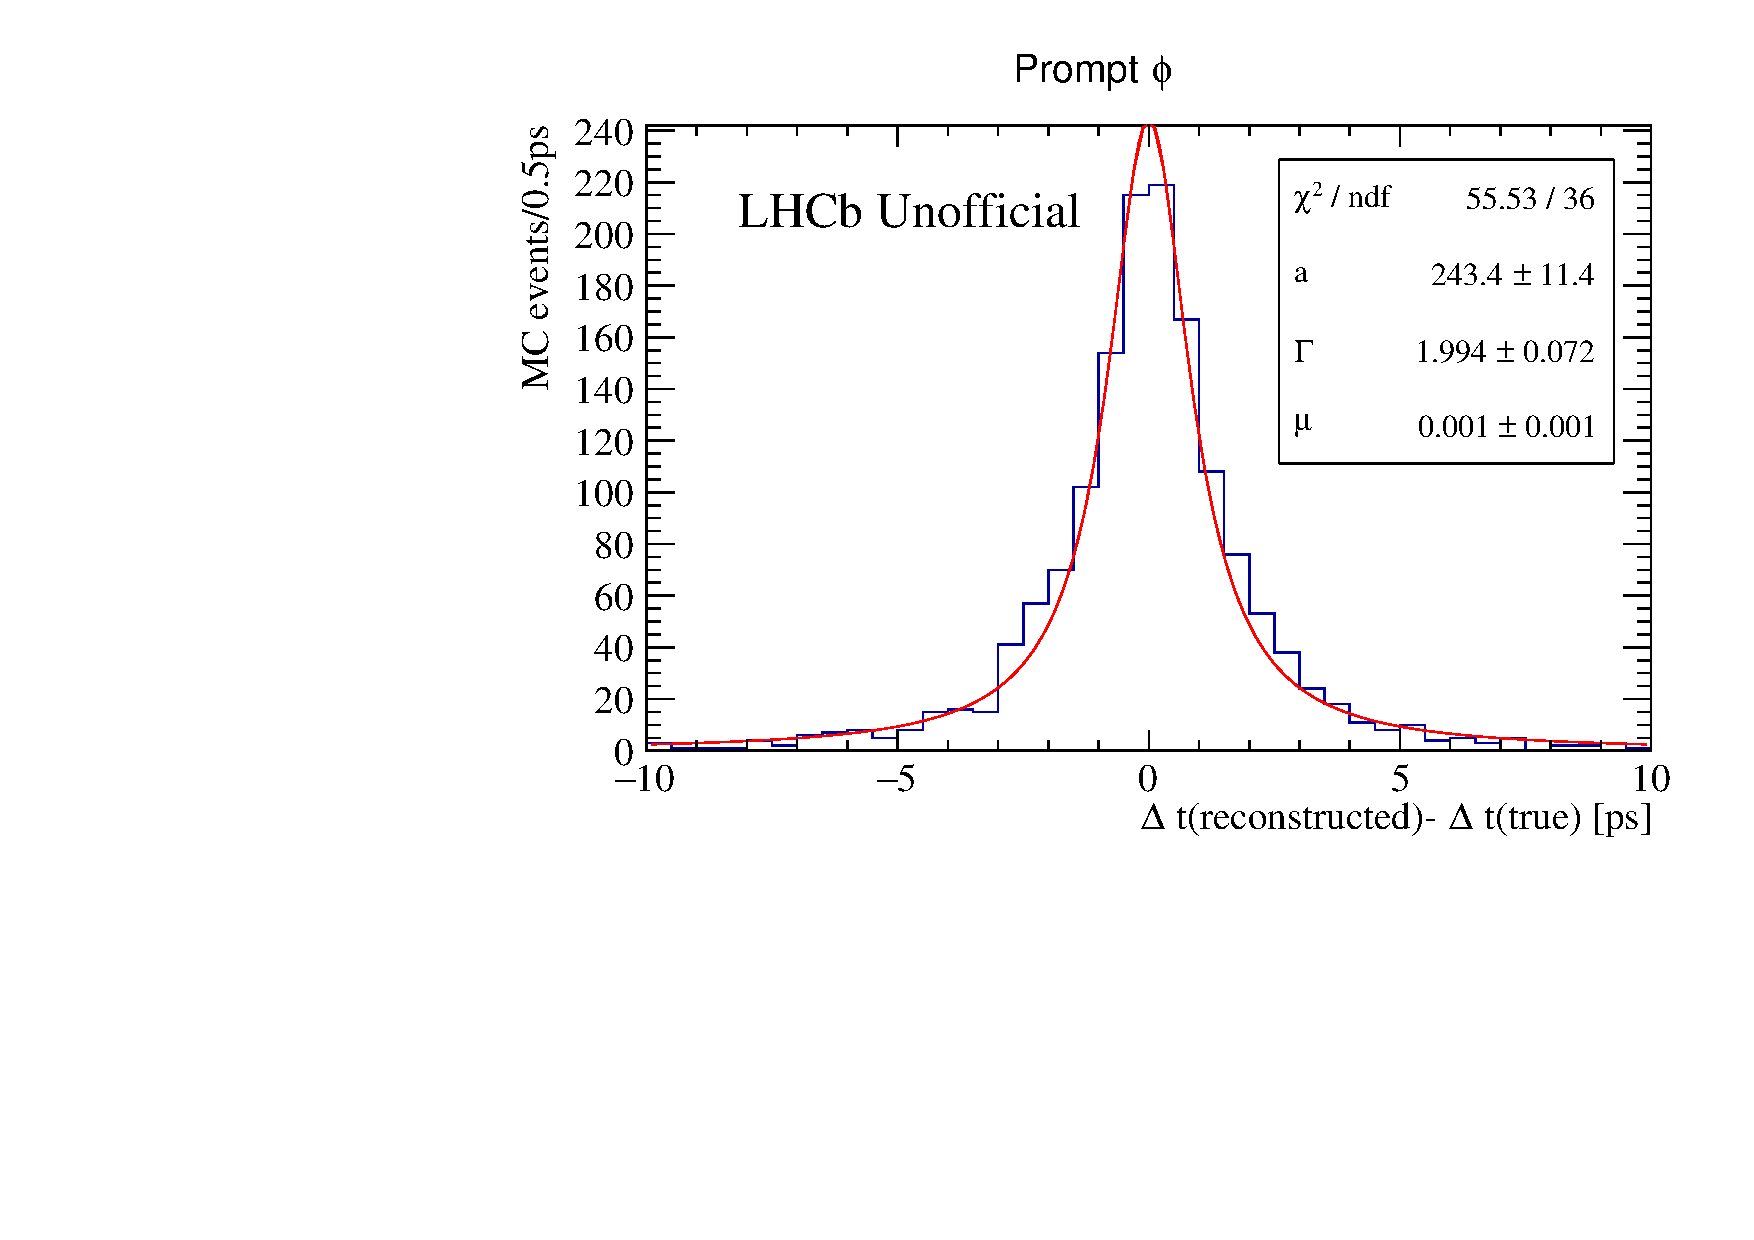
\includegraphics[width=.49\textwidth]{figs/time_res_incl/timeResolution-DeltaTauLL-DTF.pdf}
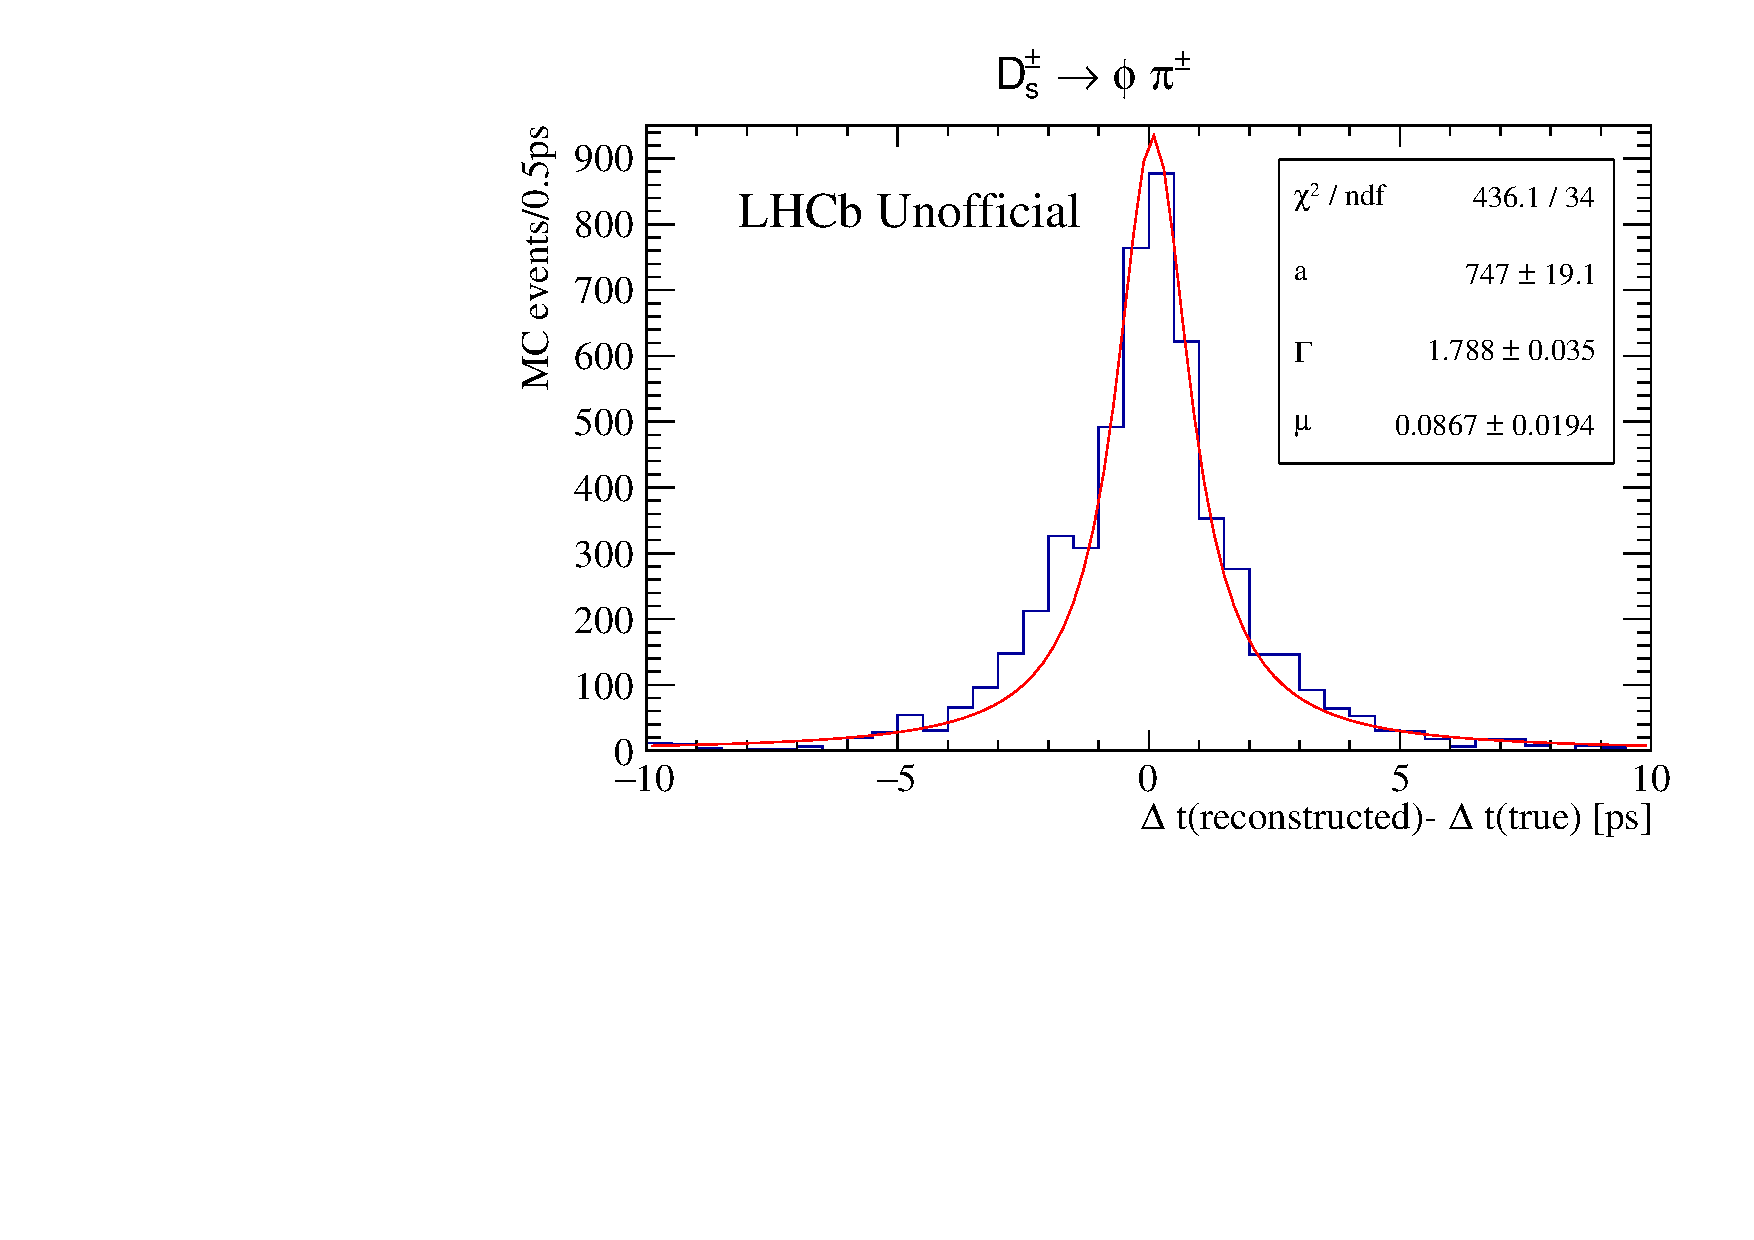
\includegraphics[width=.49\textwidth]{figs/time_res_Ds/timeResolution-DeltaTauLL-DTF.pdf}
\captionof{figure}{Resolution of $\Delta t$ reconstructed via DecayTreeFitter LL kaons. }\label{FIG:timres-LL-DTF-prof}
\end{center}

\begin{center}
\begin{tabular}{c|cc}
Distribution & Prompt $\phi$ & $D_s^\pm \rightarrow \phi \pi^\pm$ \\ 
\hline 
$t$ & $0.127\pm0.006$  & $0.627\pm0.008$ \\ 
$\Delta t$ & $1.99 \pm 0.07$ & $1.79 \pm 0.04$ \\ 
\end{tabular} 
\captionof{table}{Width $\Gamma$ [ps] of the given distributions of decay times and decay time differences for LL kaons reconstructed via the DecayTreeFitter.} \label{TAB:DTF}
\end{center}

\subsection{Using the TupleToolPropertime}
The TupleToolPropertime does not explicitly exclude negative decay times. Therefore, the difference between reconstructed and true decay time relative to the true decay time is symmetric as seen in figures \ref{FIG:LL} and \ref{FIG:DD}. The average residual of the decay time in figure \ref{FIG:all-prof} confirms this.

\begin{center}
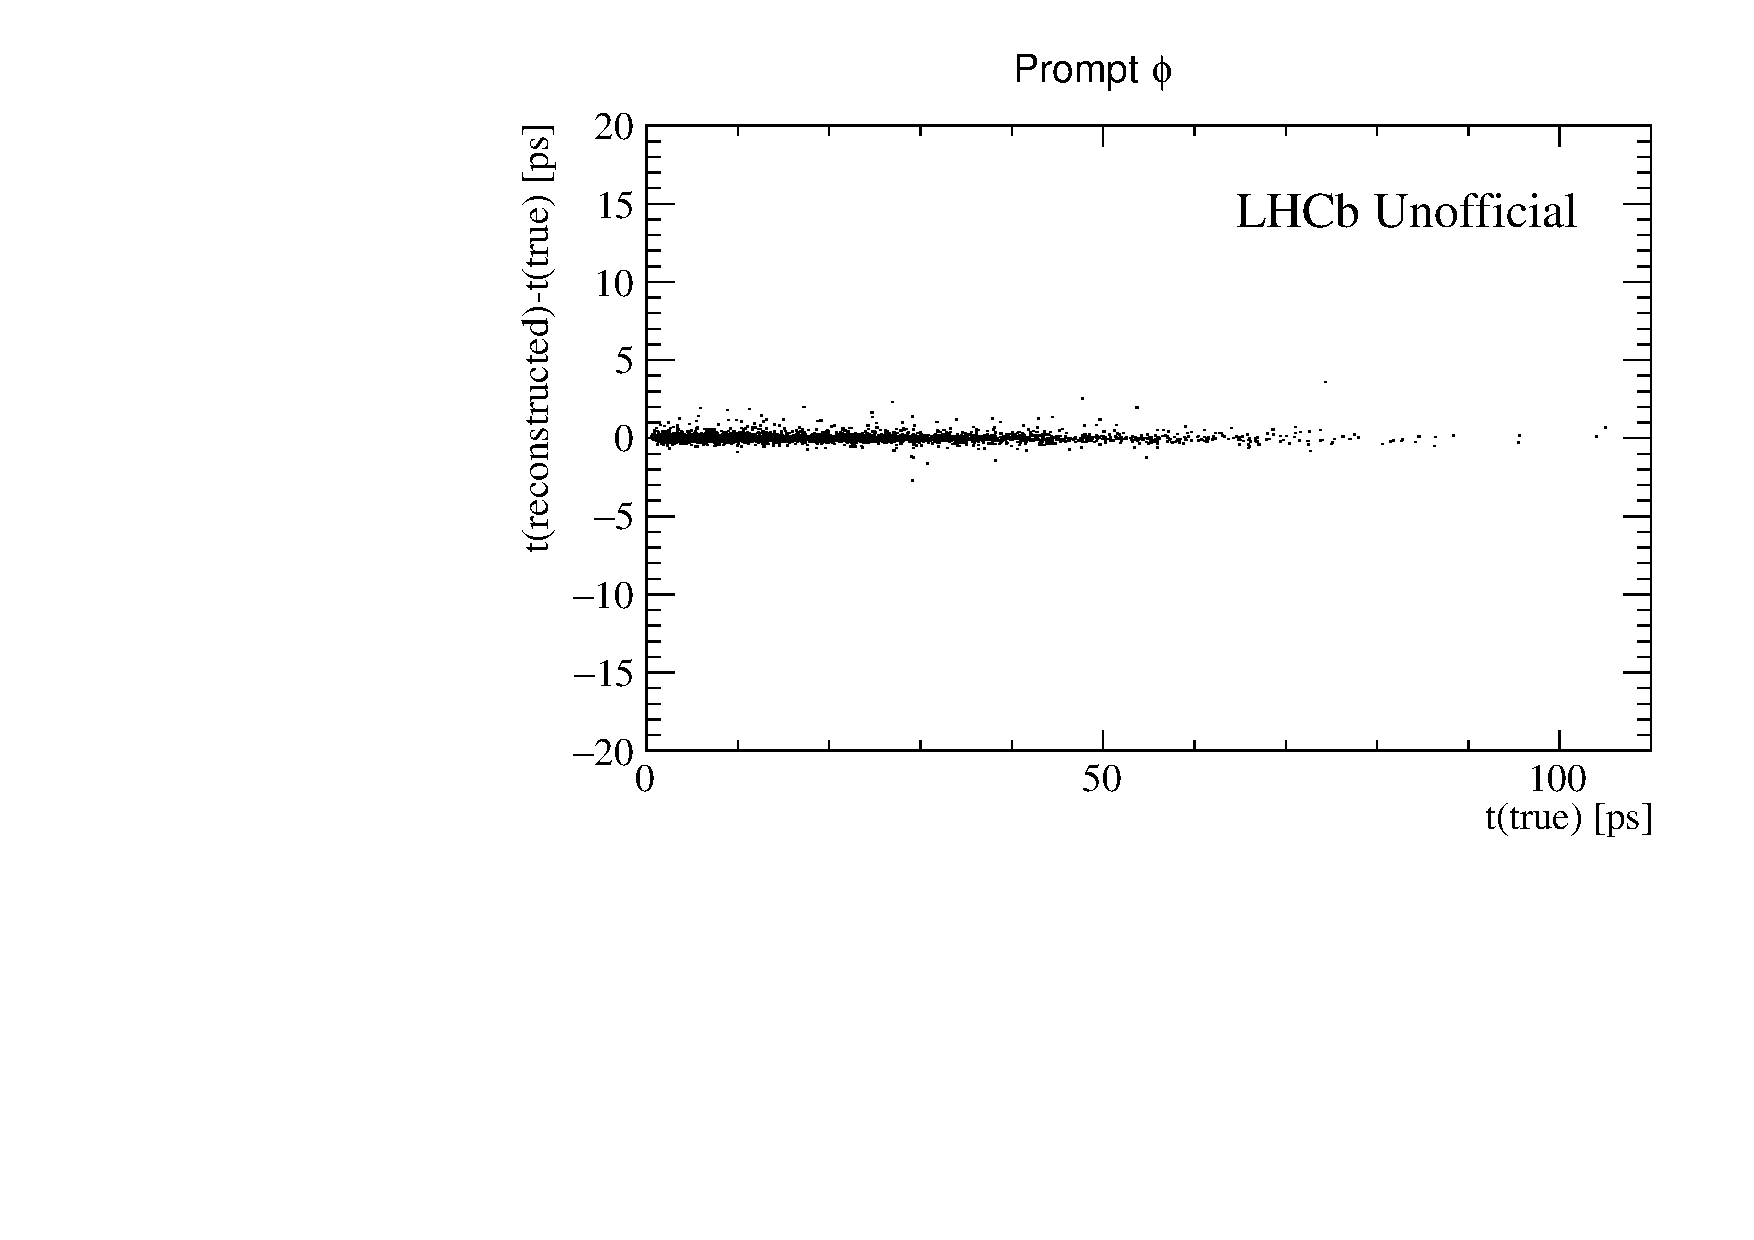
\includegraphics[width=.49\textwidth]{figs/time_res_incl/LL.pdf}
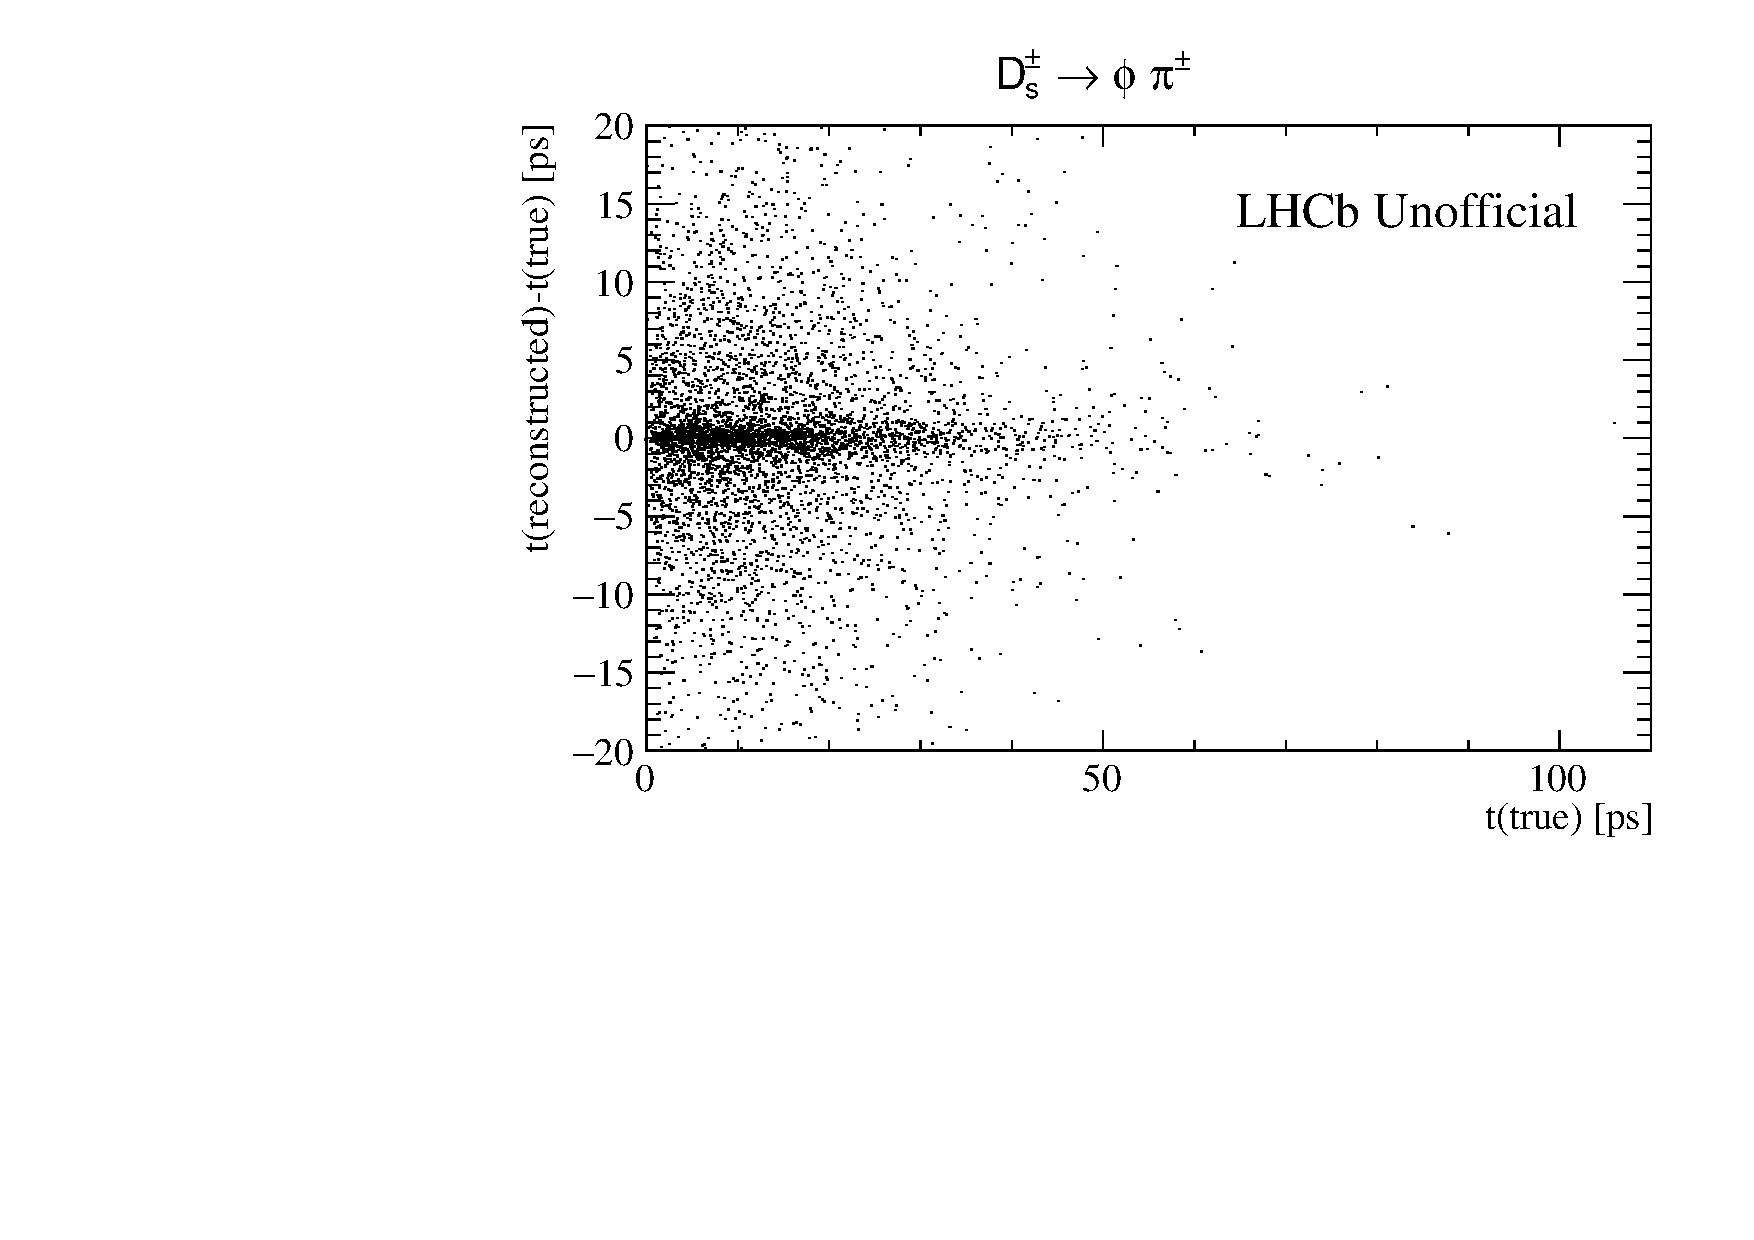
\includegraphics[width=.49\textwidth]{figs/time_res_Ds/LL.pdf}
\captionof{figure}{Residual of $t$ for LL kaons reconstructed using the TupleToolPropertime plotted against the true value of $t$. }\label{FIG:LL}

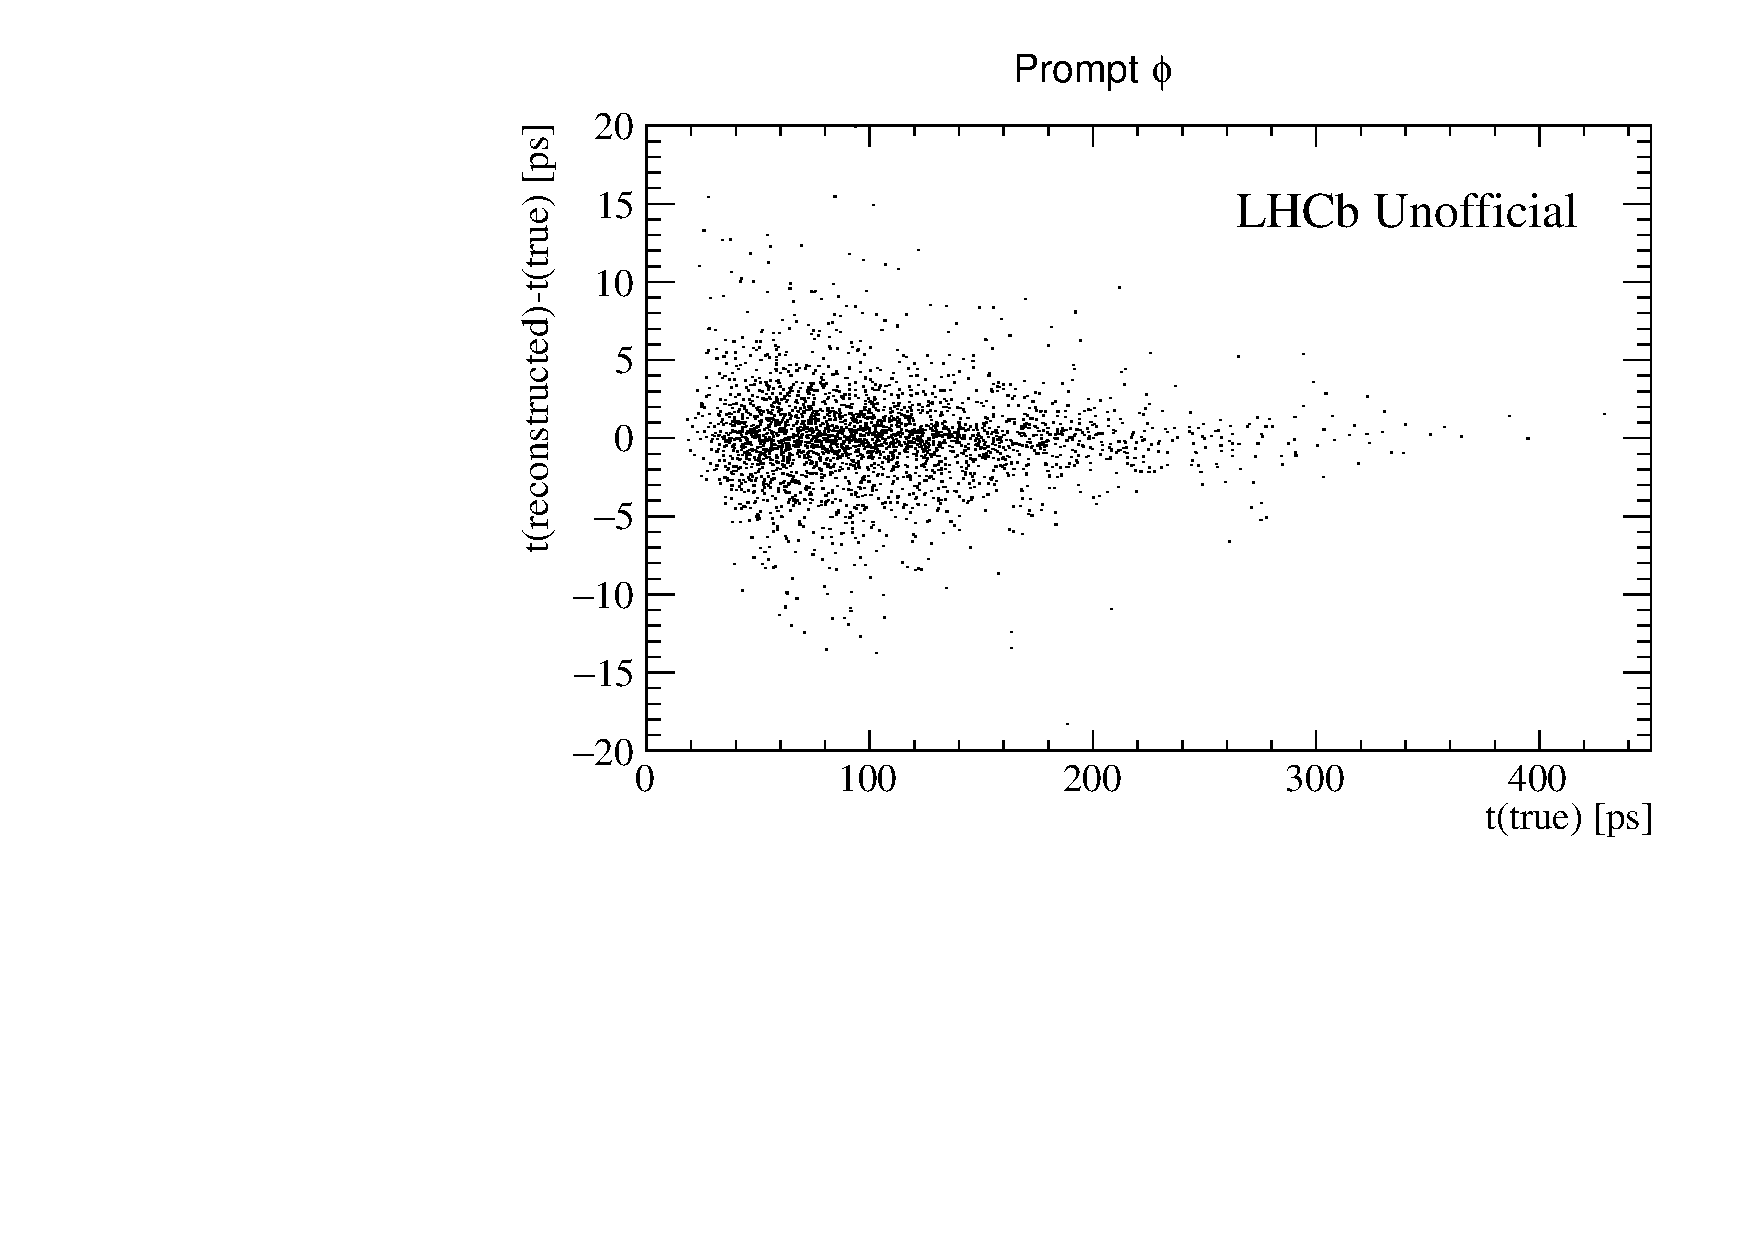
\includegraphics[width=.49\textwidth]{figs/time_res_incl/DD.pdf}
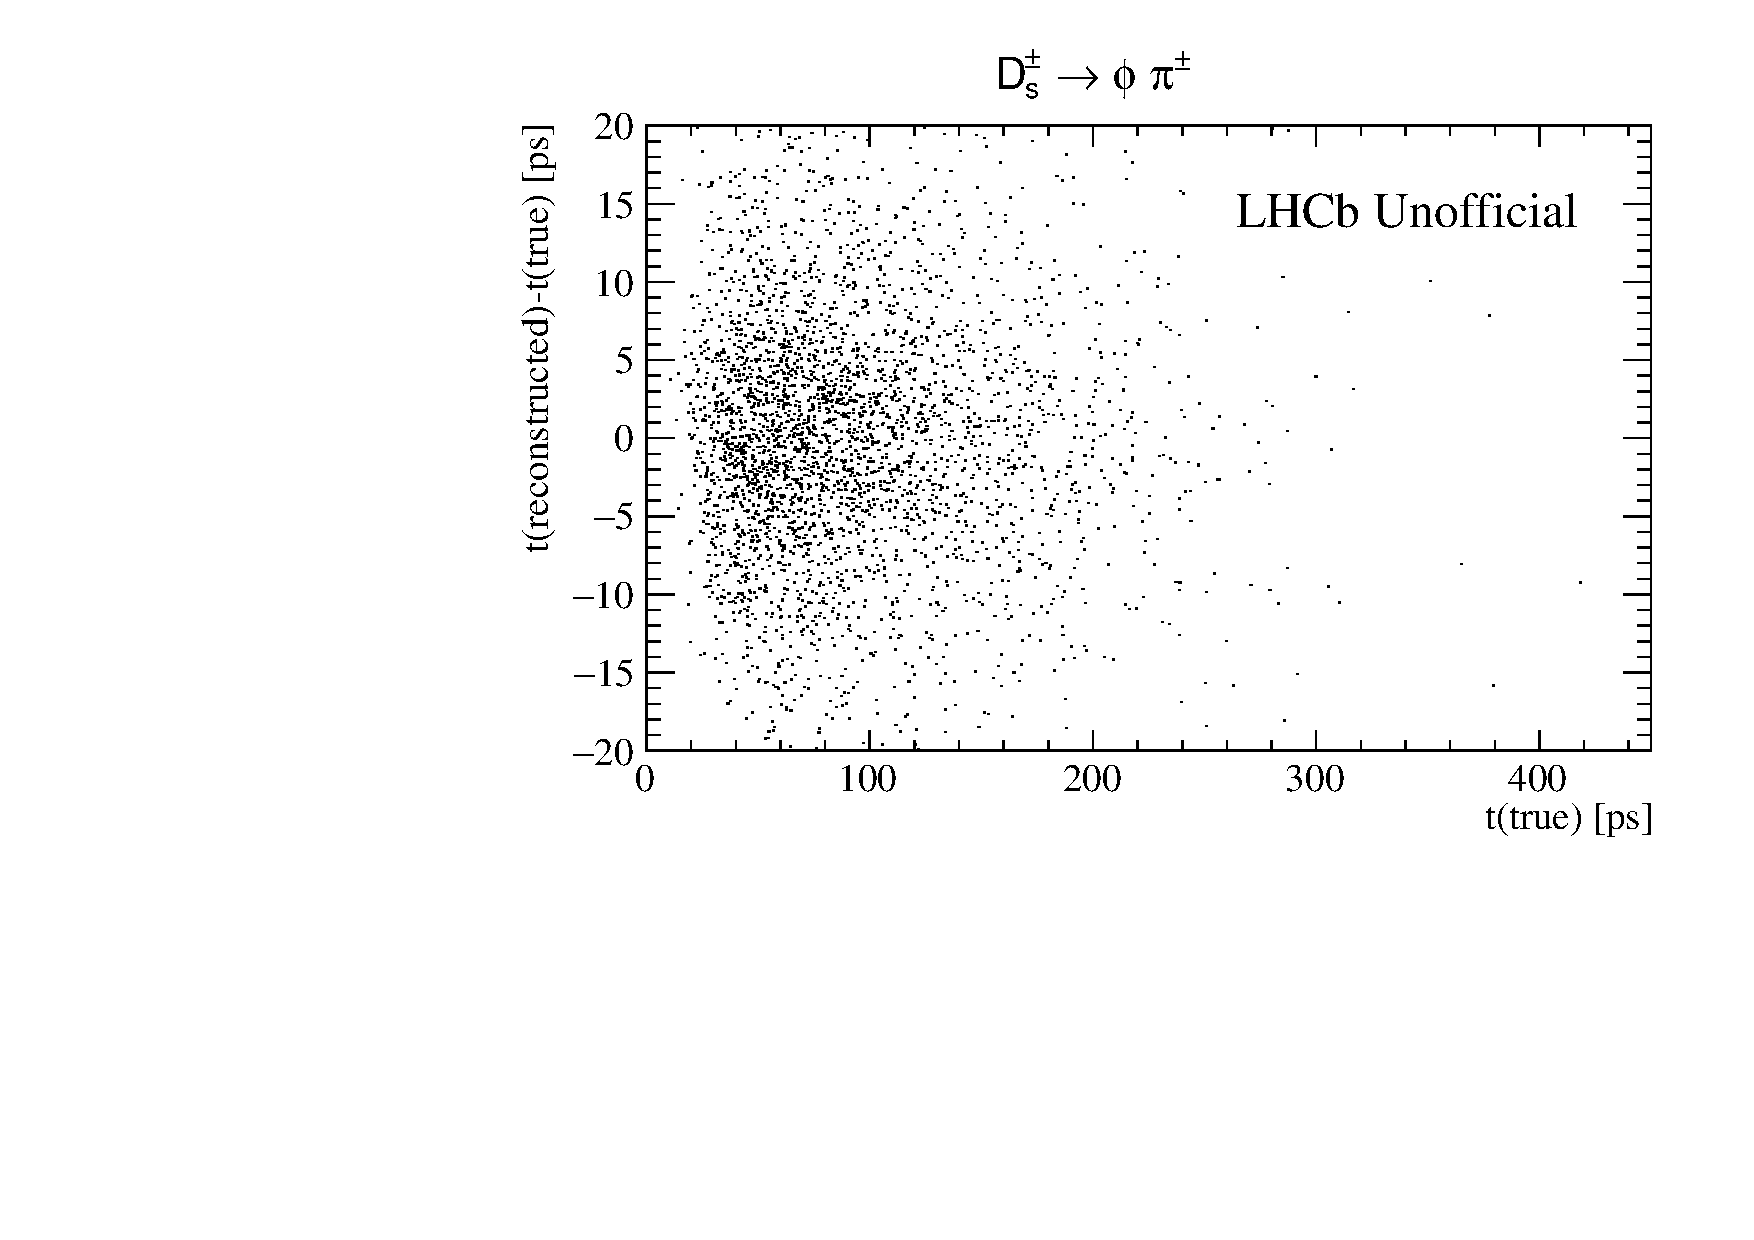
\includegraphics[width=.49\textwidth]{figs/time_res_Ds/DD.pdf}
\captionof{figure}{Residual of $t$ for DD kaons reconstructed using TupleToolPropertime plotted against the true value of $t$.}\label{FIG:DD}
\end{center}


\begin{center}
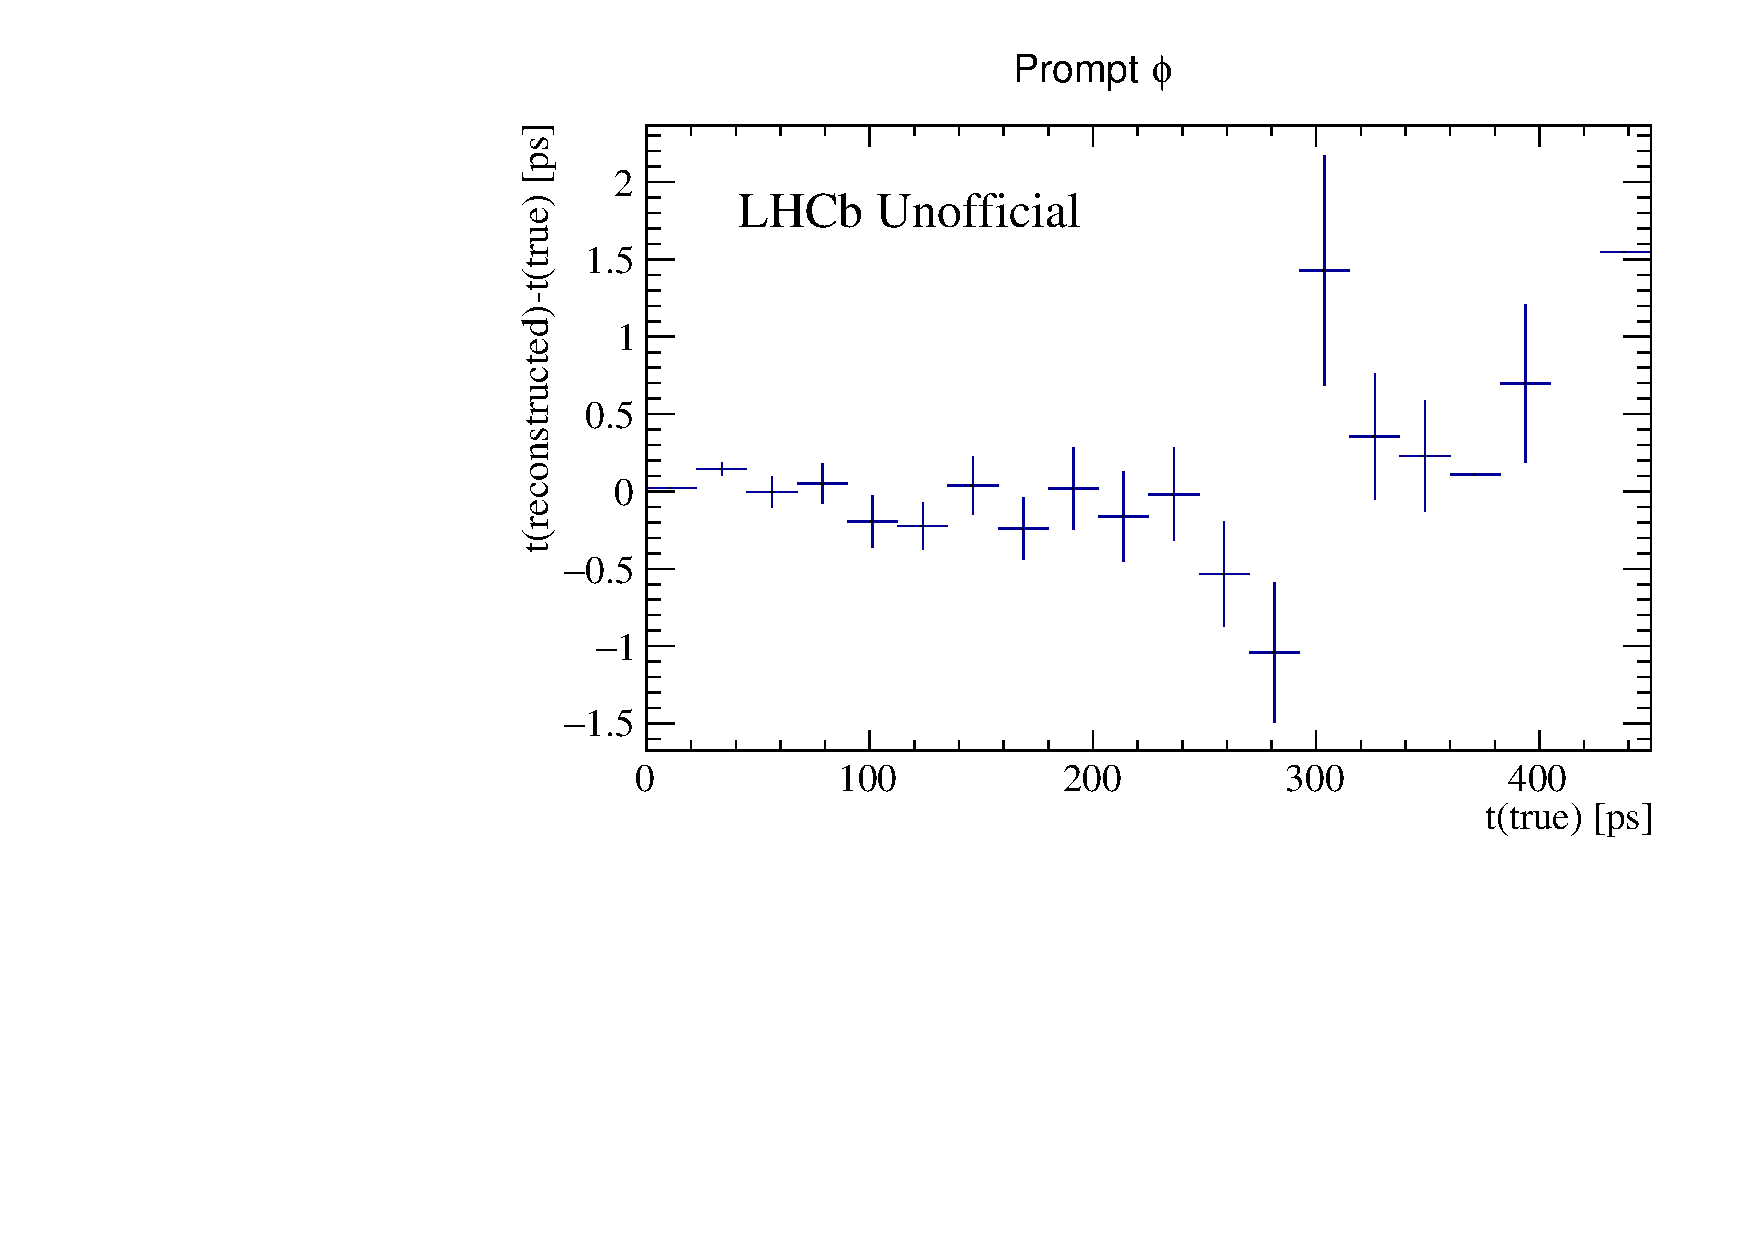
\includegraphics[width=.49\textwidth]{figs/time_res_incl/all-prof.pdf}
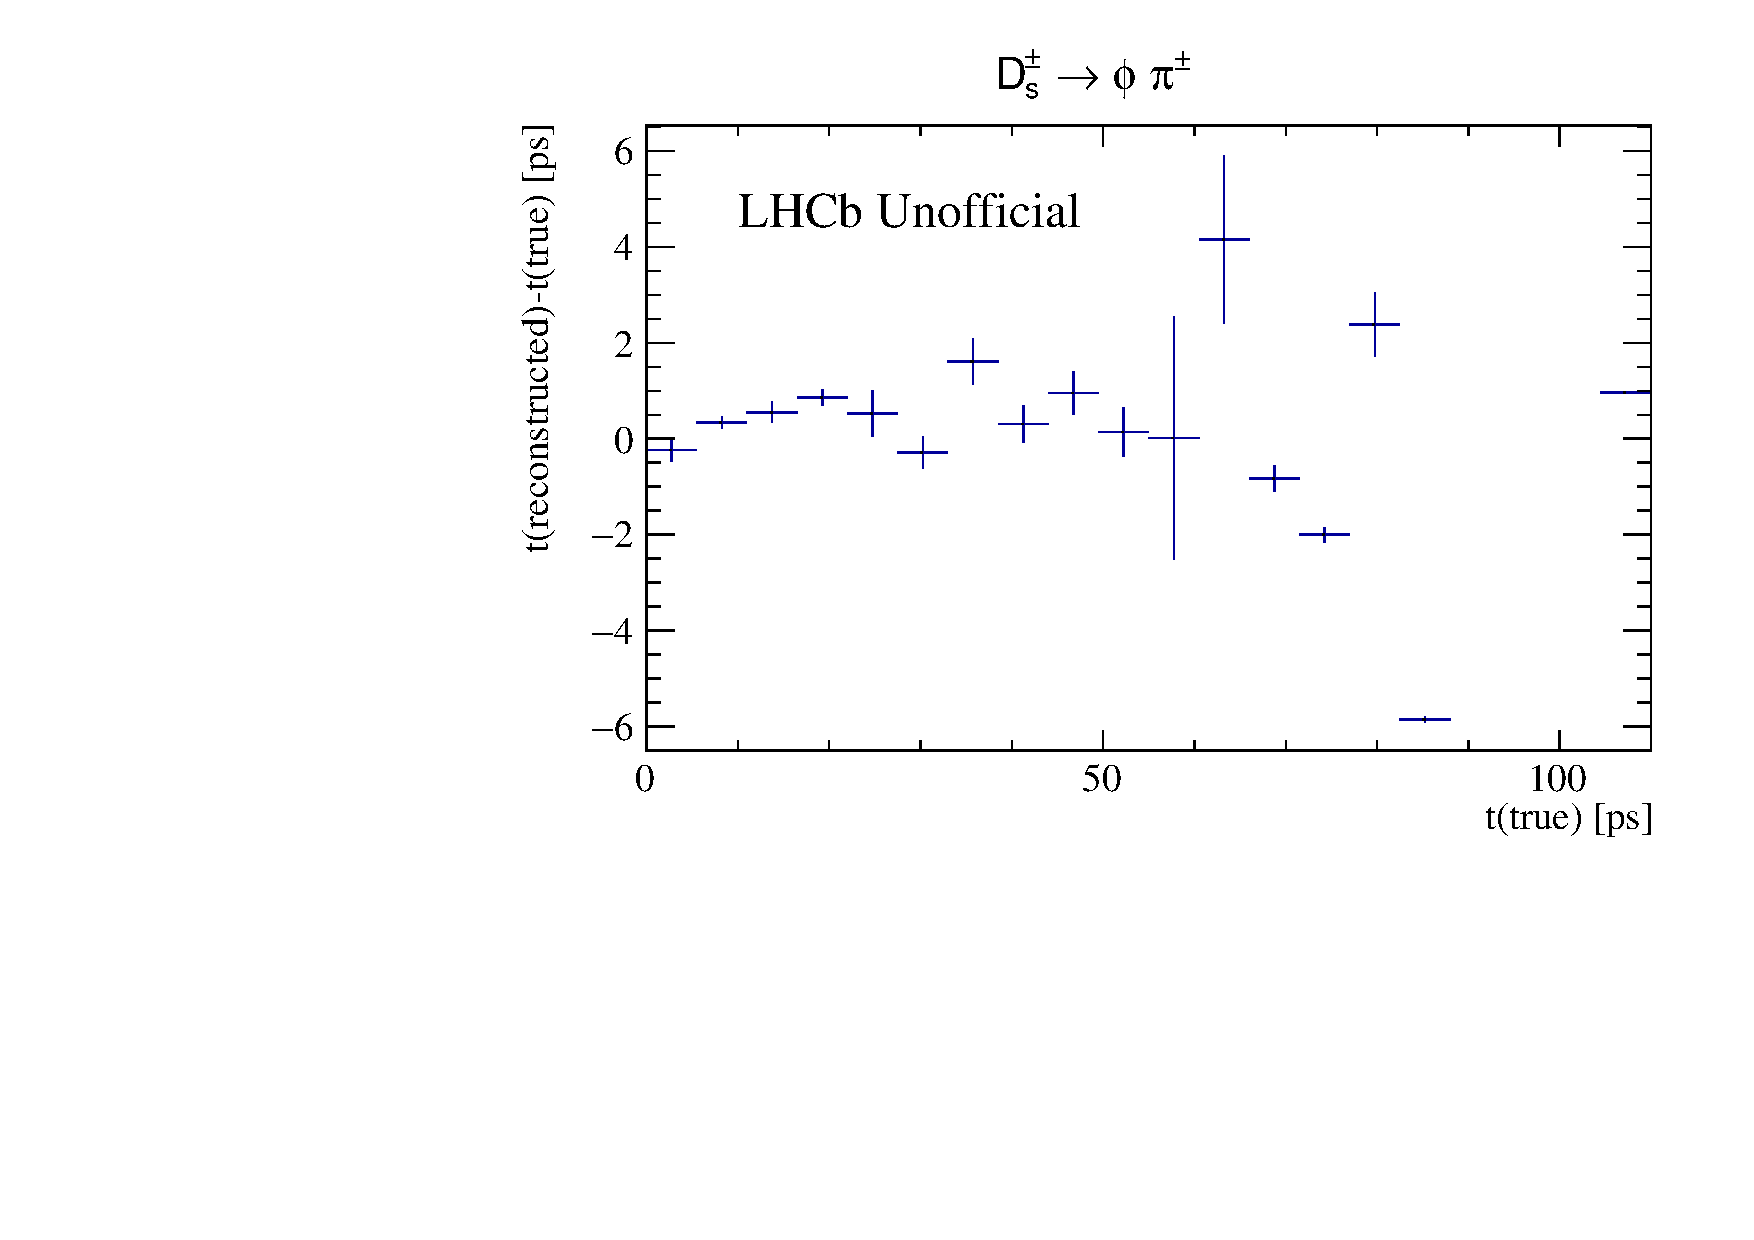
\includegraphics[width=.49\textwidth]{figs/time_res_Ds/LL-prof.pdf}
\captionof{figure}{Average of $t$ reconstructed using TupleToolPropertime for all kaons plotted against the true value of $t$.}\label{FIG:all-prof}
\end{center}
The decay time resolution has been fitted to the Breit Wigner distribution in equation \eqref{EQ:BWt} as shown in figures \ref{FIG:LL-res} and \ref{FIG:DD-res} with the following results for the width:

\begin{center}
\begin{tabular}{c|cc}
& Prompt $\phi$ & $D_s^\pm\rightarrow \phi \pi^\pm$ \\ 
\hline 
LL& $0.126 \pm 0.003$ & $1.55 \pm 0.04$ \\ 
DD& $2.54 \pm 0.07$ & $10.64 \pm 0.14$ \\ 
\end{tabular} 
\captionof{table}{Width $\Gamma$ [ps] of the time resolution for the reconstruction with TupleToolPropertime.}
\end{center}

\begin{center}
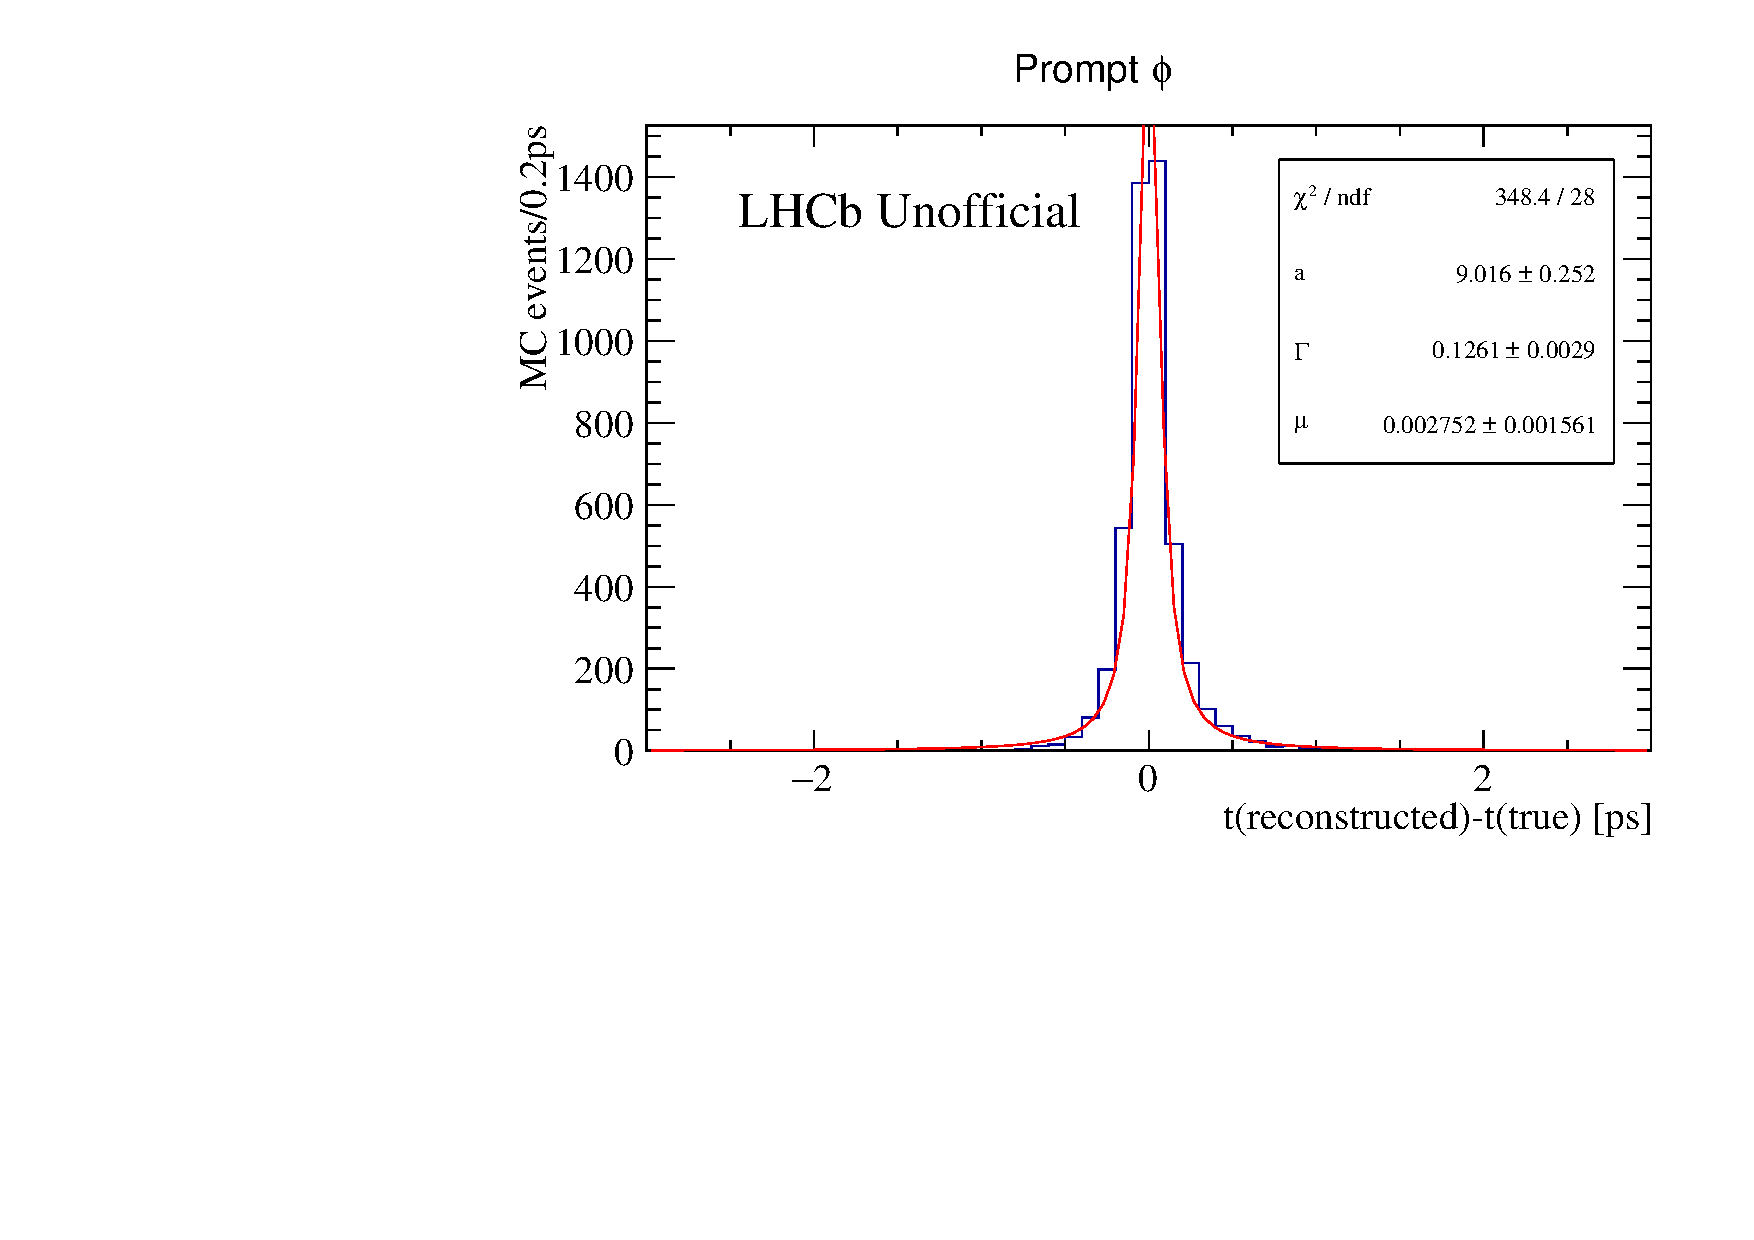
\includegraphics[width=.49\textwidth]{figs/time_res_incl/timeResolution-LL.pdf}
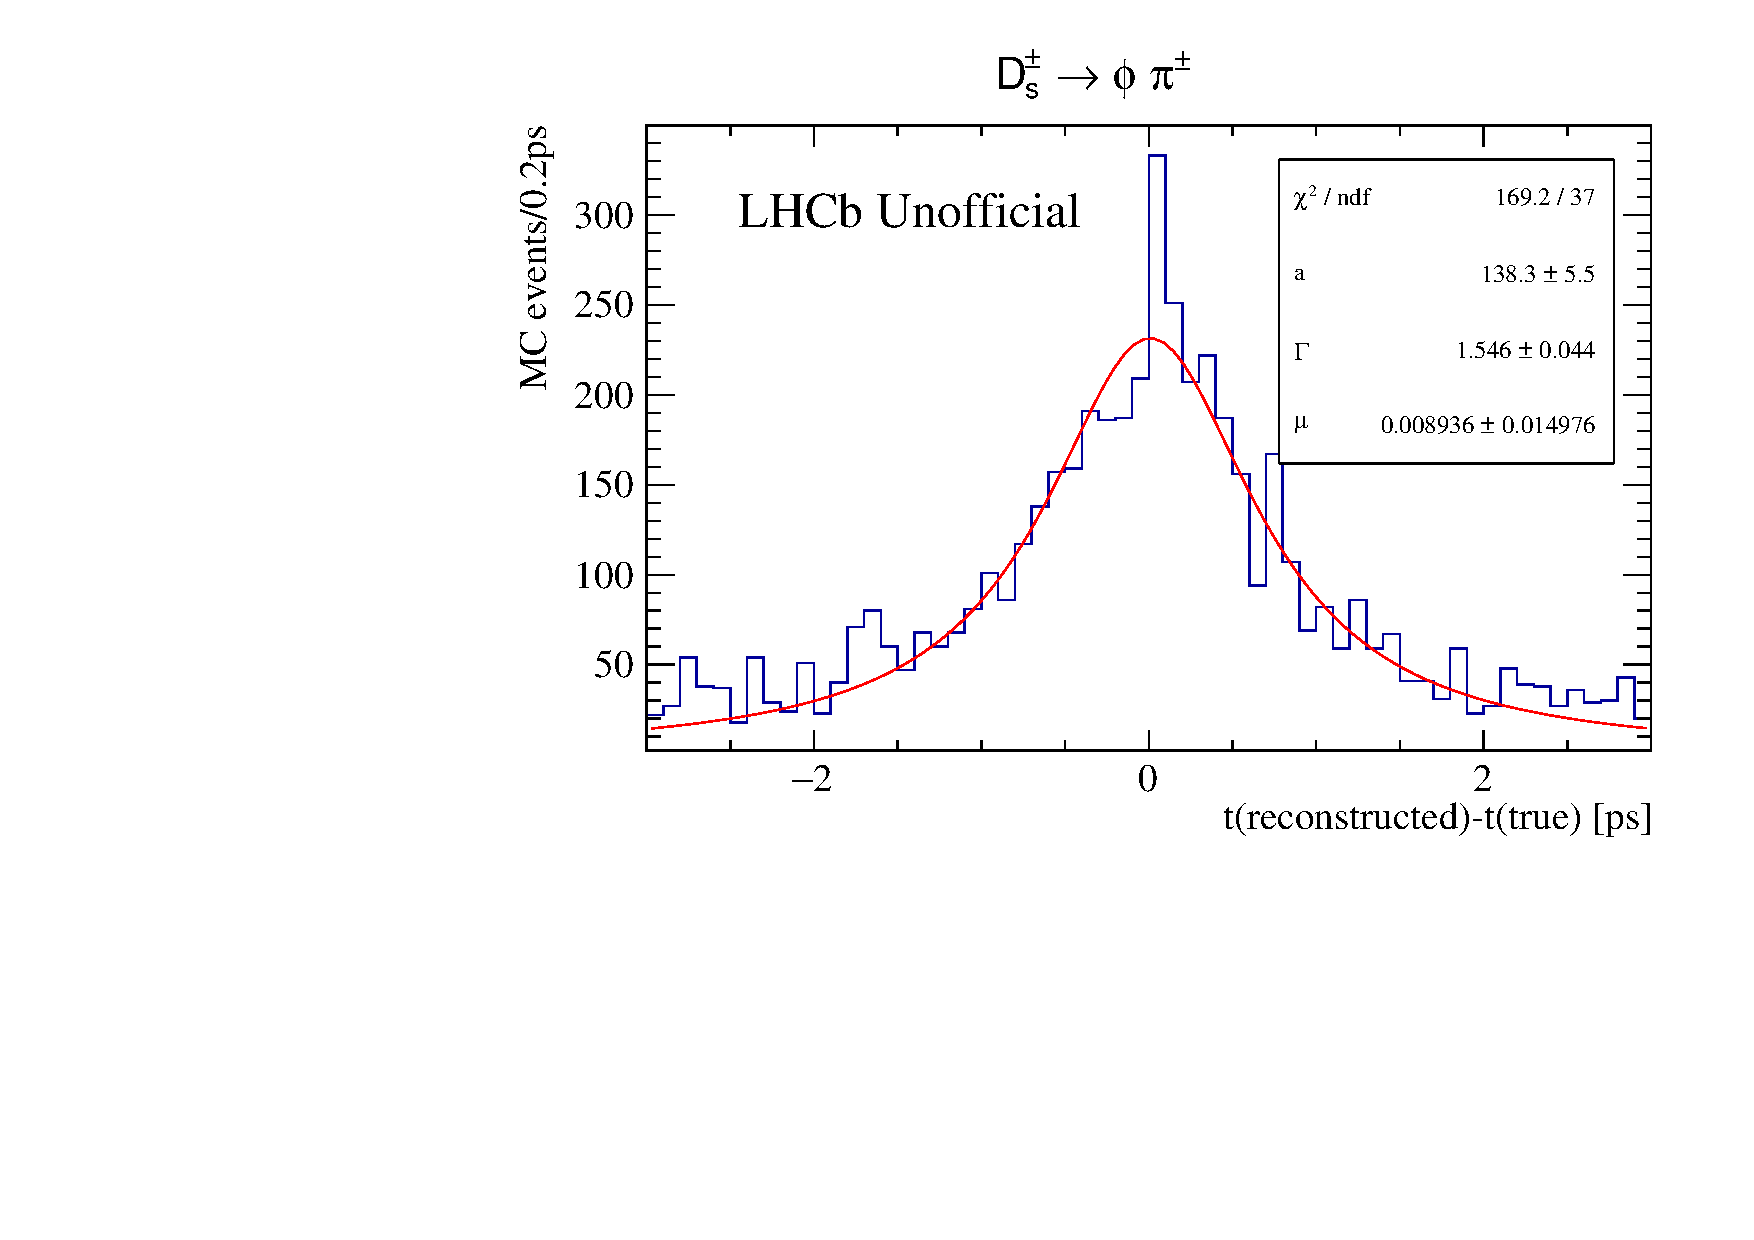
\includegraphics[width=.49\textwidth]{figs/time_res_Ds/timeResolution-LL.pdf}
\captionof{figure}{Resolution of LL kaon decay times $t$ reconstructed via the DecayTreeFitter. }\label{FIG:LL-res}


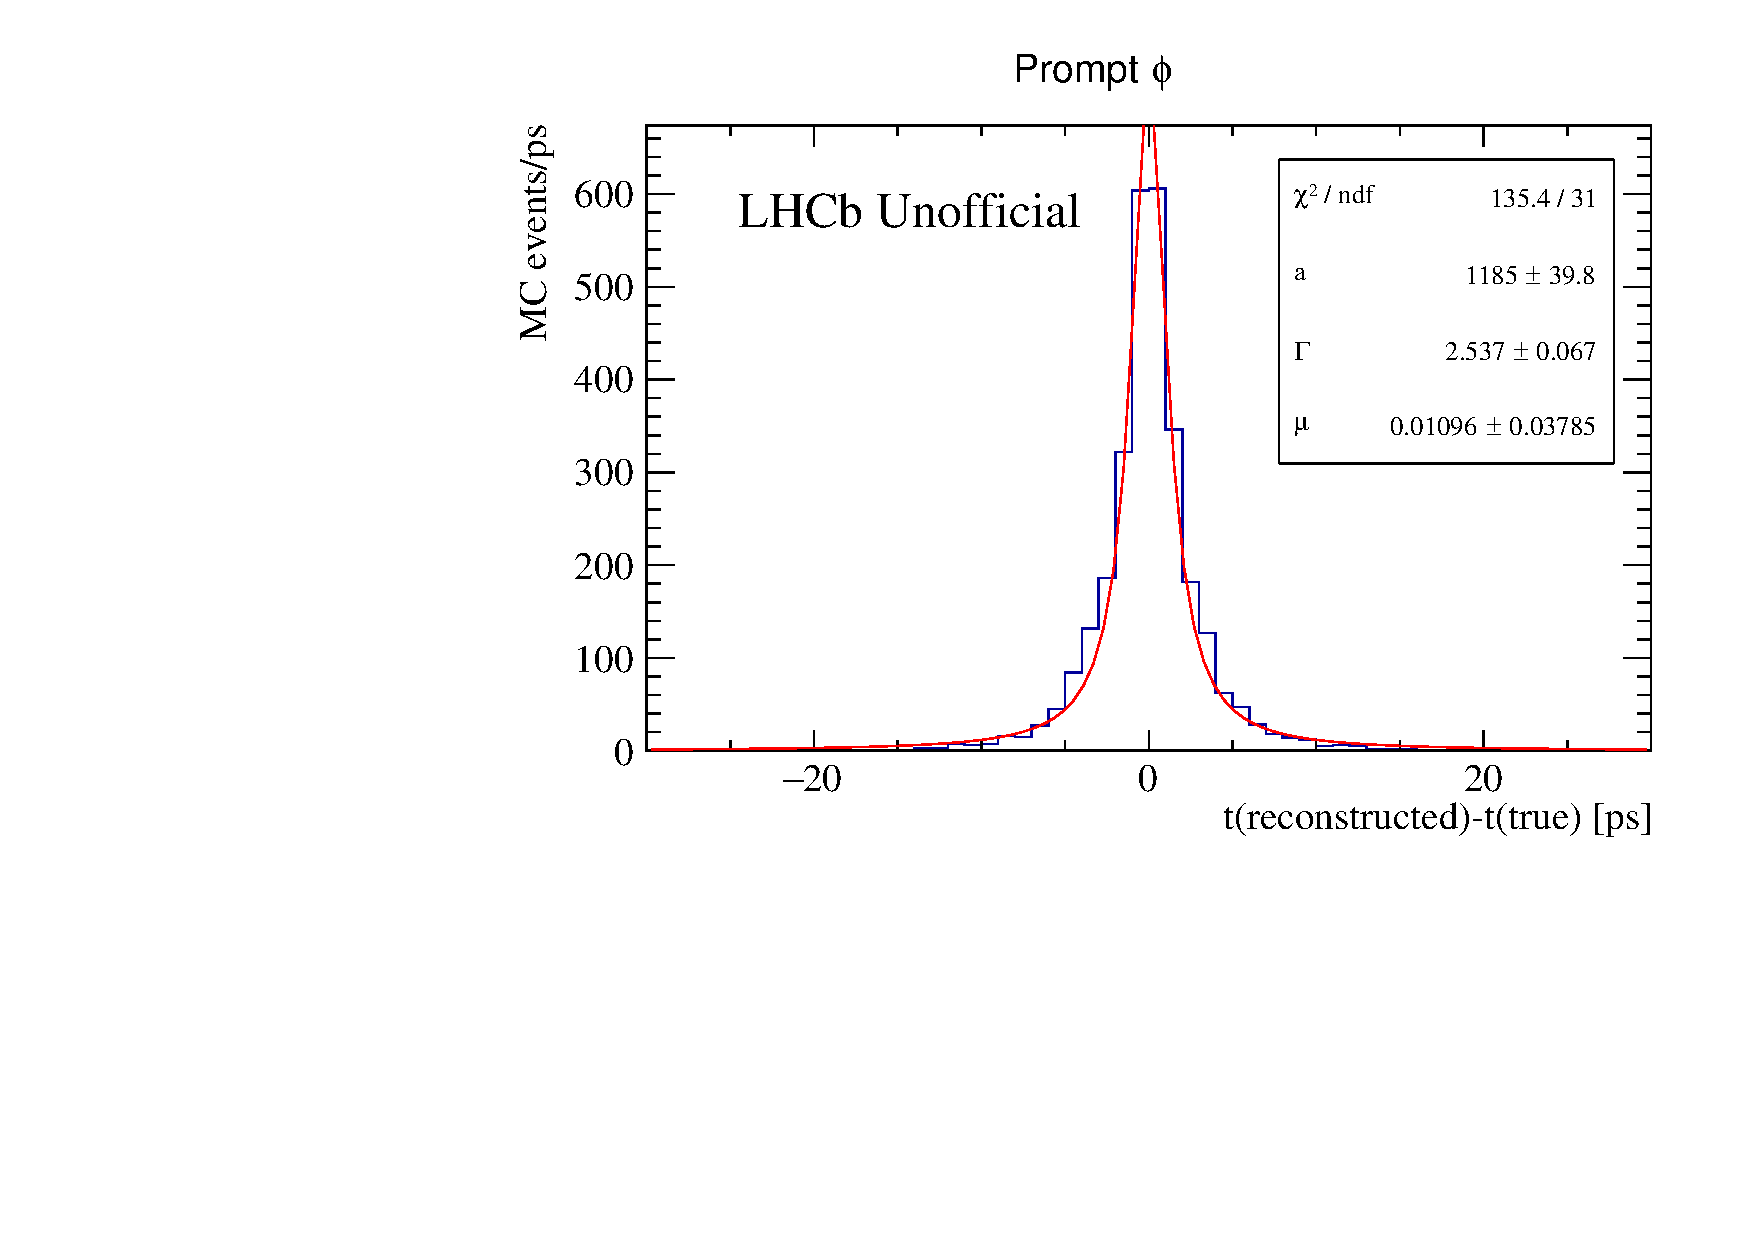
\includegraphics[width=.49\textwidth]{figs/time_res_incl/timeResolution-DD.pdf}
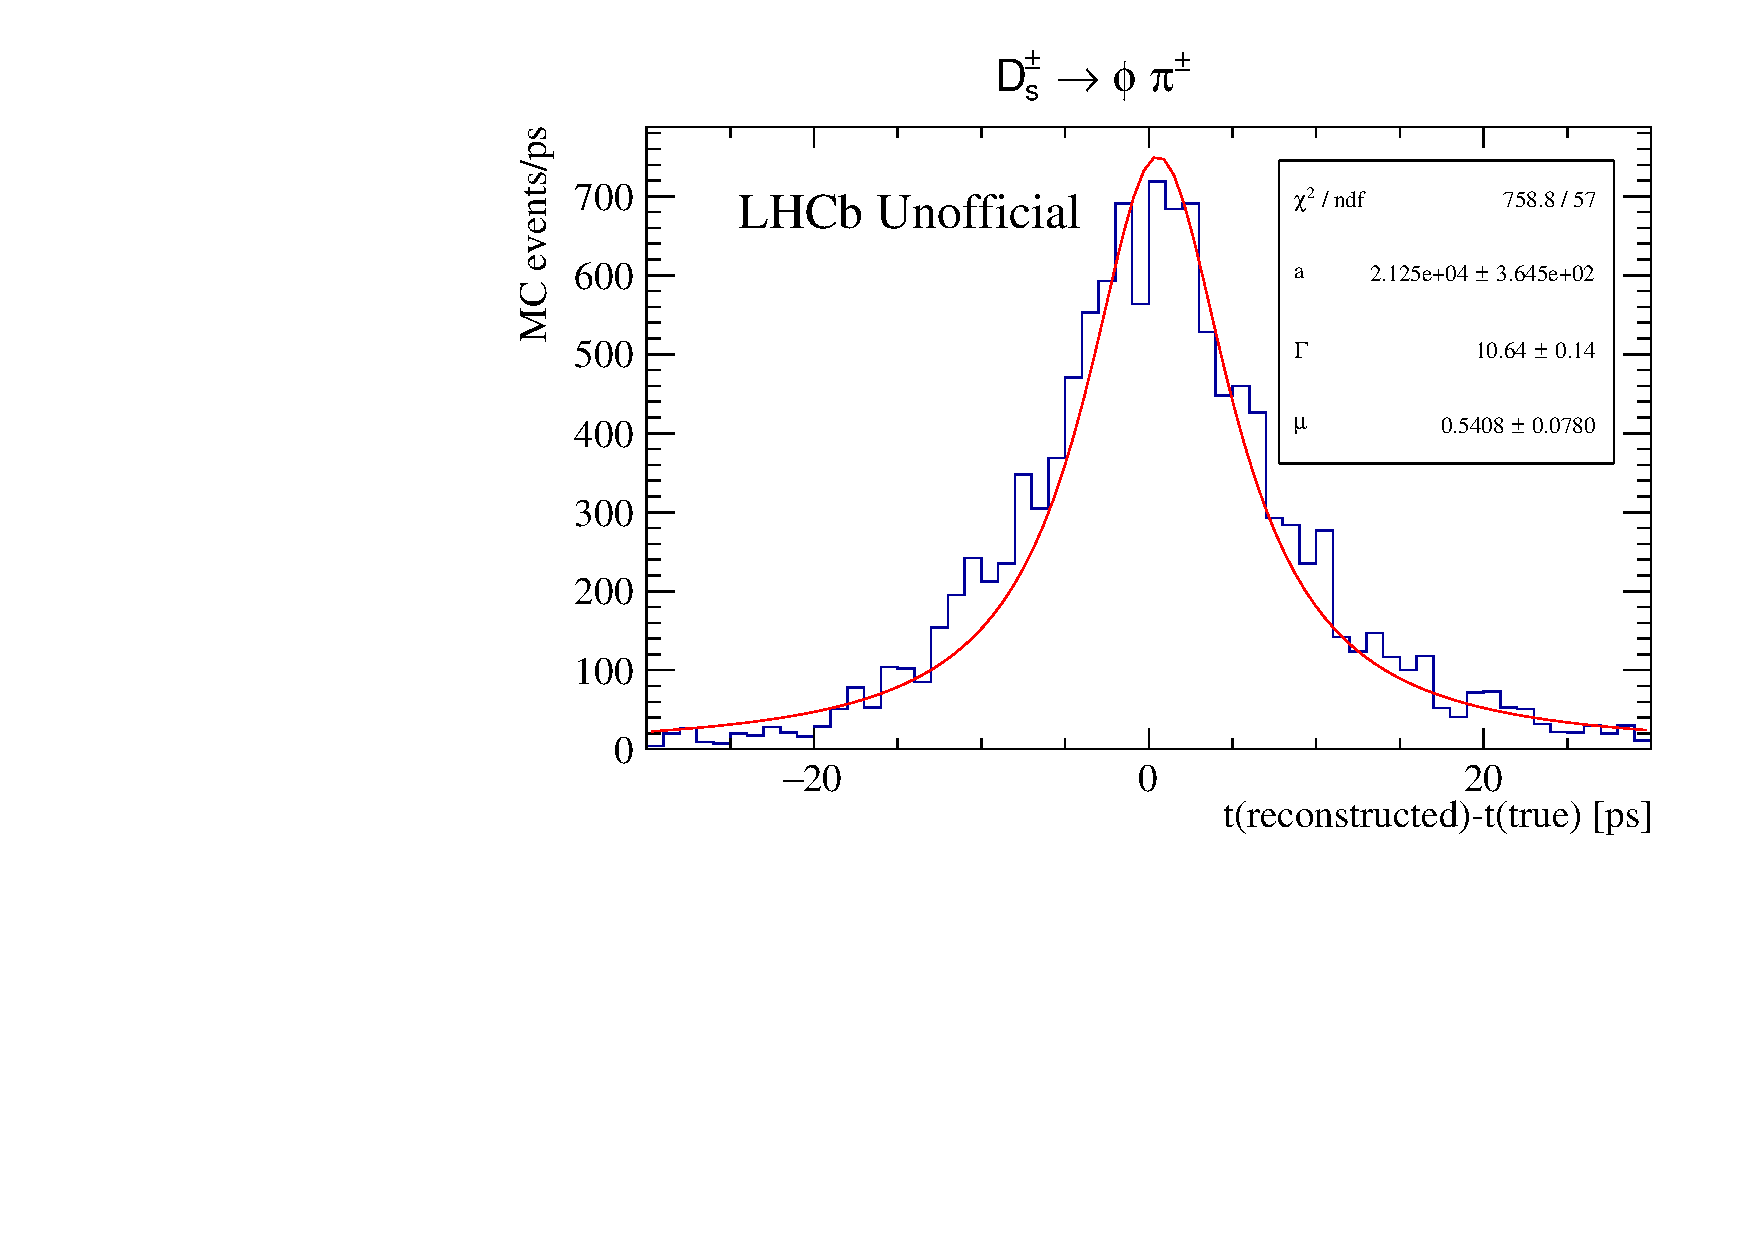
\includegraphics[width=.49\textwidth]{figs/time_res_Ds/timeResolution-DD.pdf}
\captionof{figure}{Resolution of DD kaon decay times $t$ reconstructed via the DecayTreeFitter.  }\label{FIG:DD-res}
\end{center}

Additionally, the resolution of $\Delta t$ has been determined by fitting the Breit Wigner distribution in equation \eqref{EQ:BWdeltat} to the distribution of the residuals. Since in the Monte Carlo either both kaons are LL or one is LL and the other is DD, here, these two combinations have been studied. The plots illustrating the fit can be found in figures \ref{FIG:LL-diff} and \ref{FIG:LD-diff} and the widths in table \ref{TAB:whatever}.



\begin{center}
\begin{tabular}{c|cc}
 & Prompt $\phi$ & $D_s^\pm \rightarrow \phi \pi^\pm$ \\ 
\hline 
LL and LL & $0.24 \pm 0.01$ & $0.43 \pm 0.01$ \\ 
LL and DD & $2.47 \pm 0.06$ & $4.11 \pm 0.05$ \\ 
\end{tabular} 
\captionof{table}{Width $\Gamma$ [ps] of the  decay time differences for kaons reconstructed using the TupleToolPropertime.} \label{TAB:whatever}
\end{center}


\begin{center}
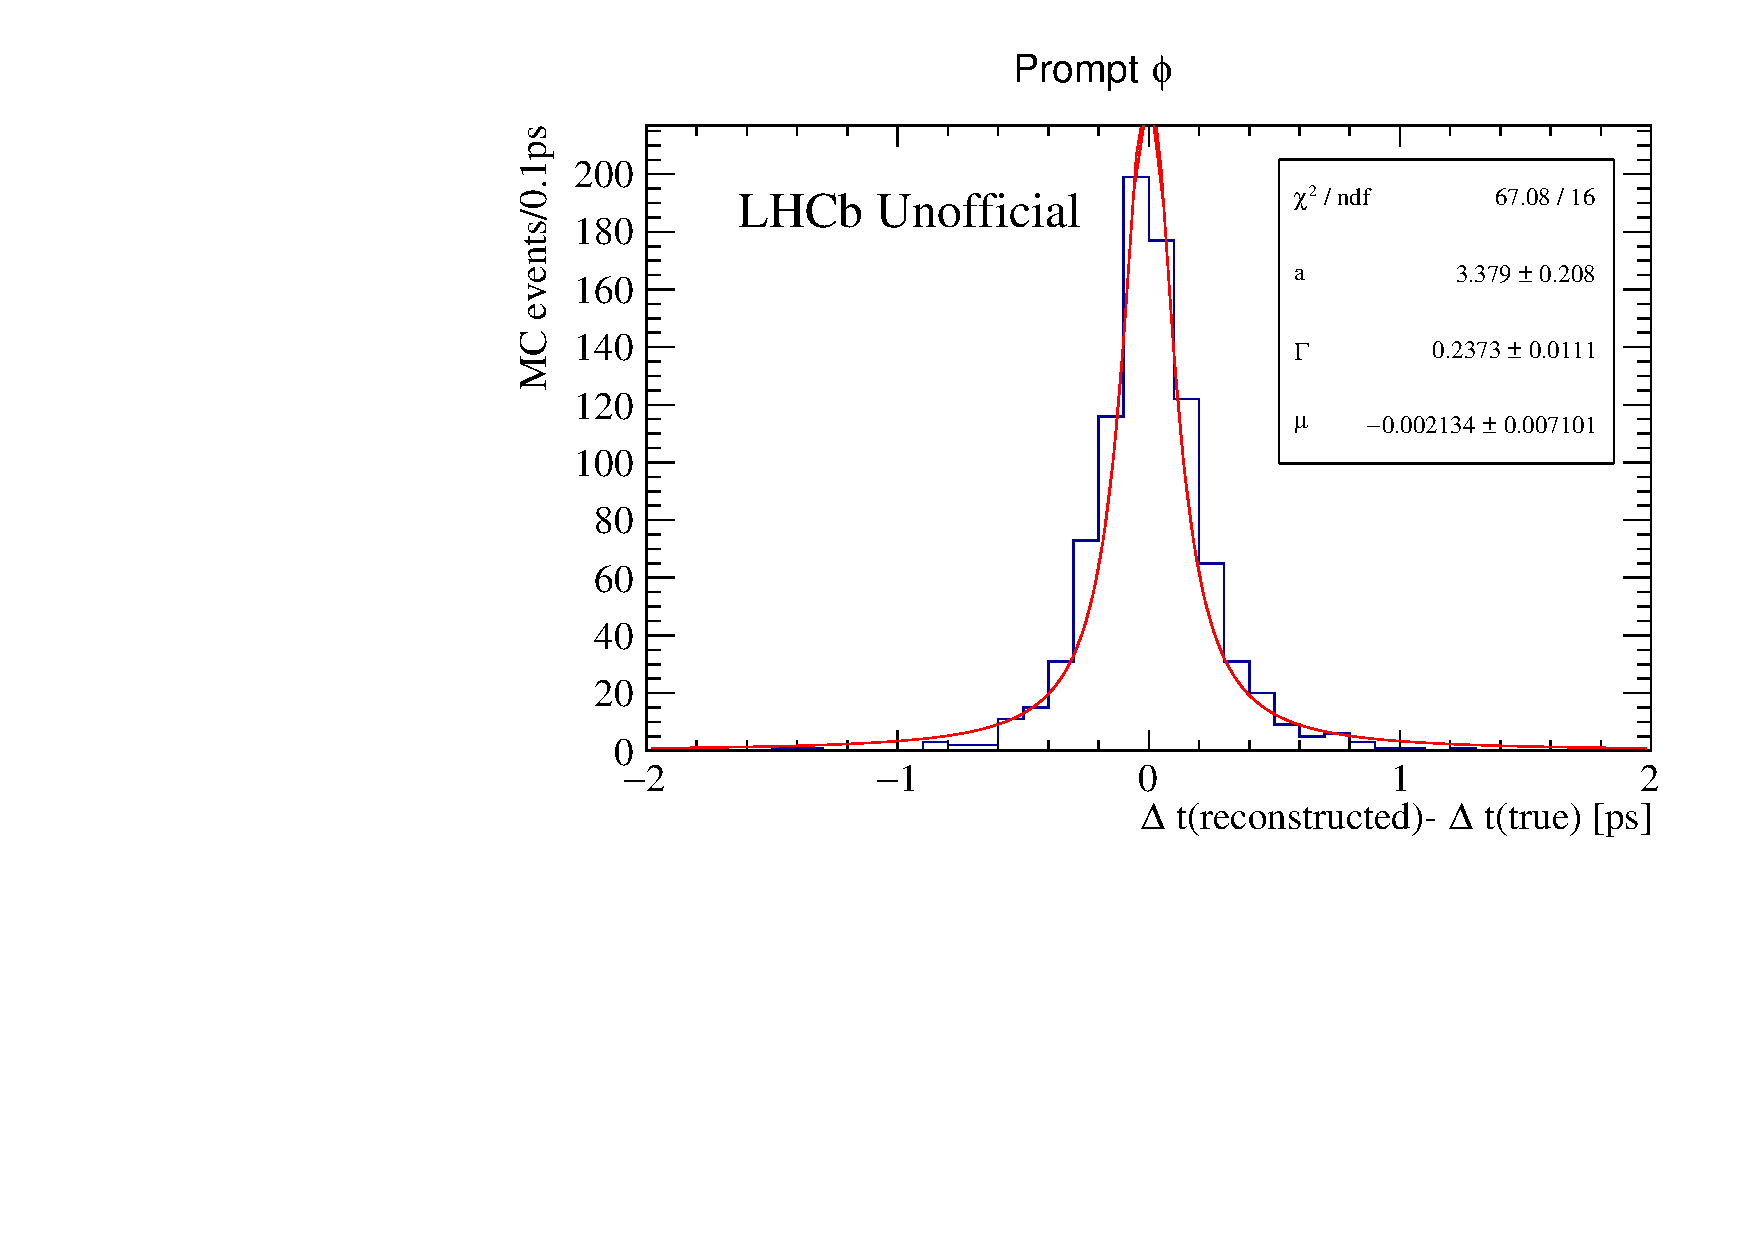
\includegraphics[width=.49\textwidth]{figs/time_res_incl/timeResolution-DeltaTauLL.pdf}
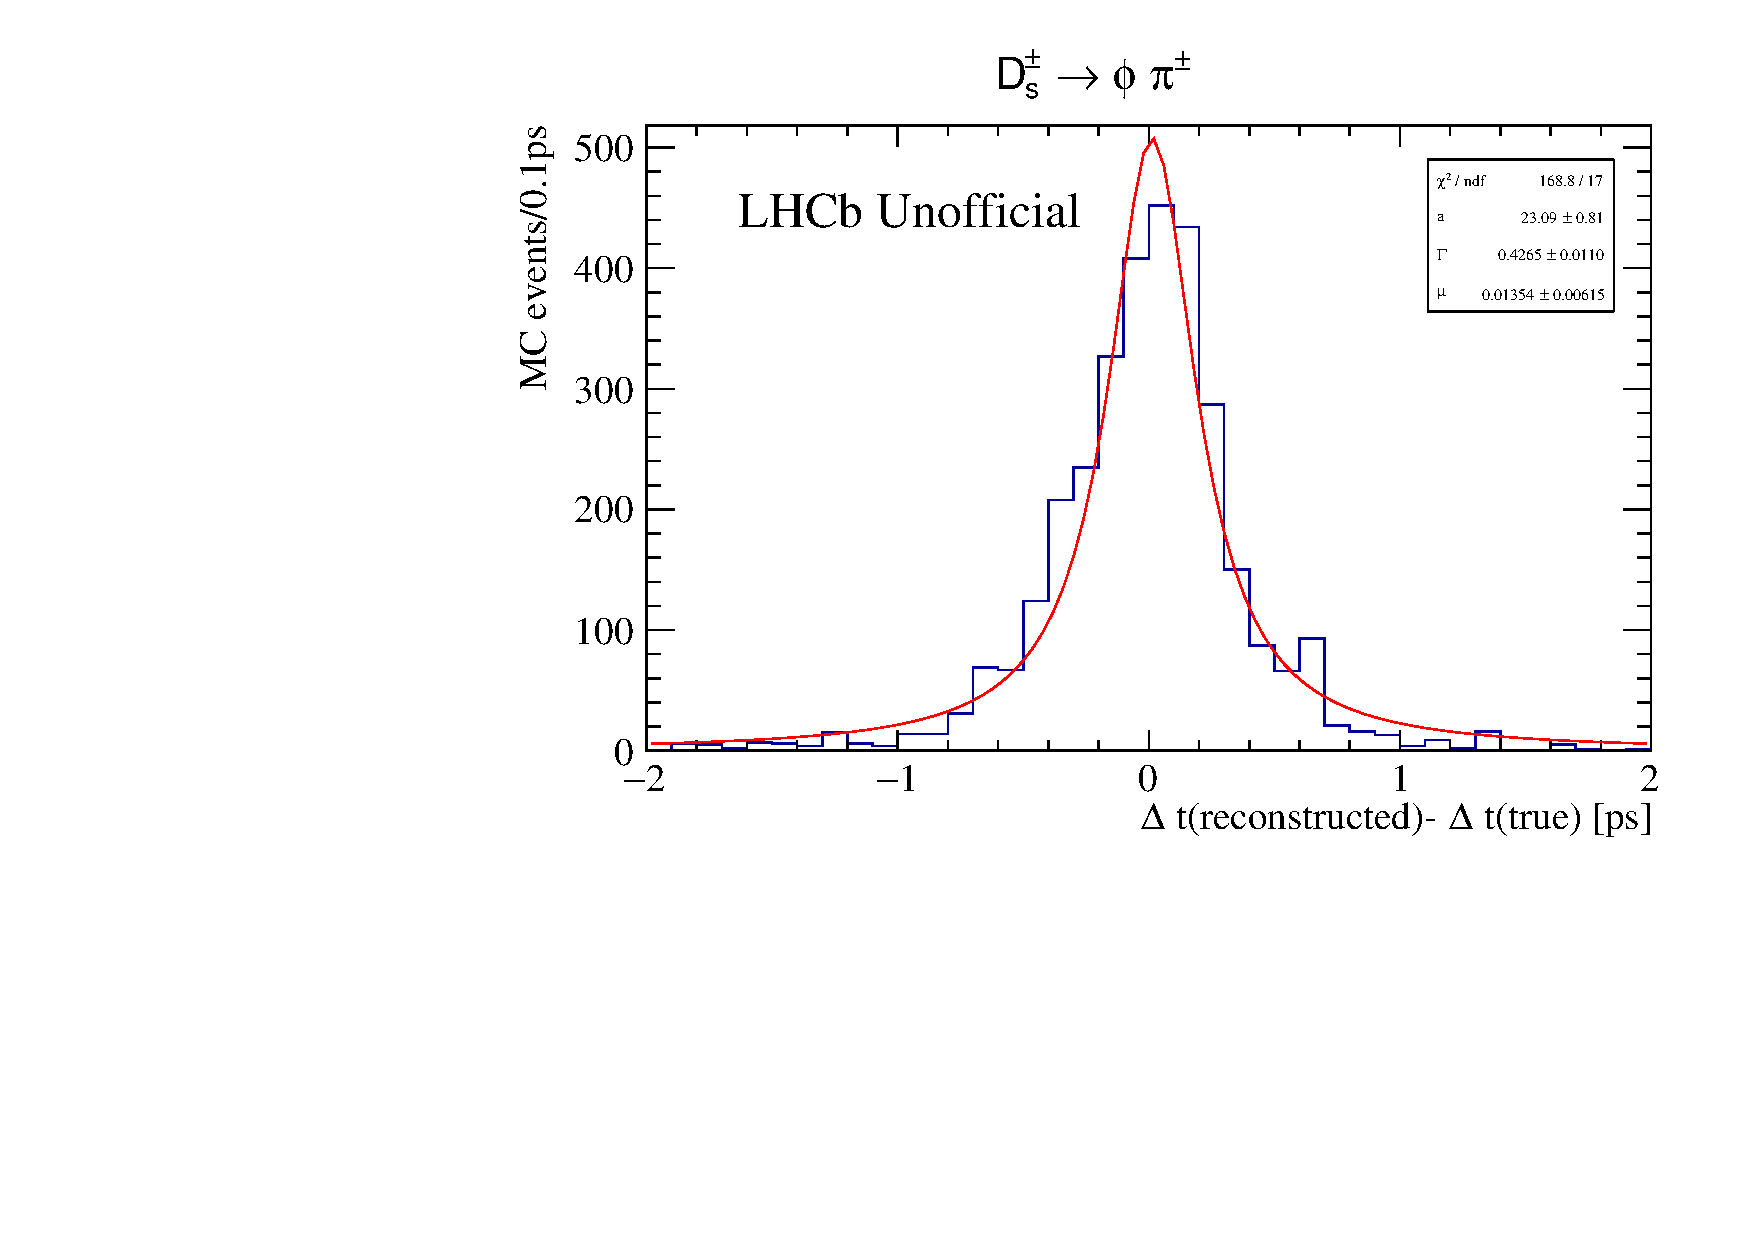
\includegraphics[width=.49\textwidth]{figs/time_res_Ds/timeResolution-DeltaTauLL.pdf}
\captionof{figure}{Resolution of $\Delta t$ for LL kaons reconstructed using the TupleToolPropertime. }\label{FIG:LL-diff}
\end{center}


\begin{center}
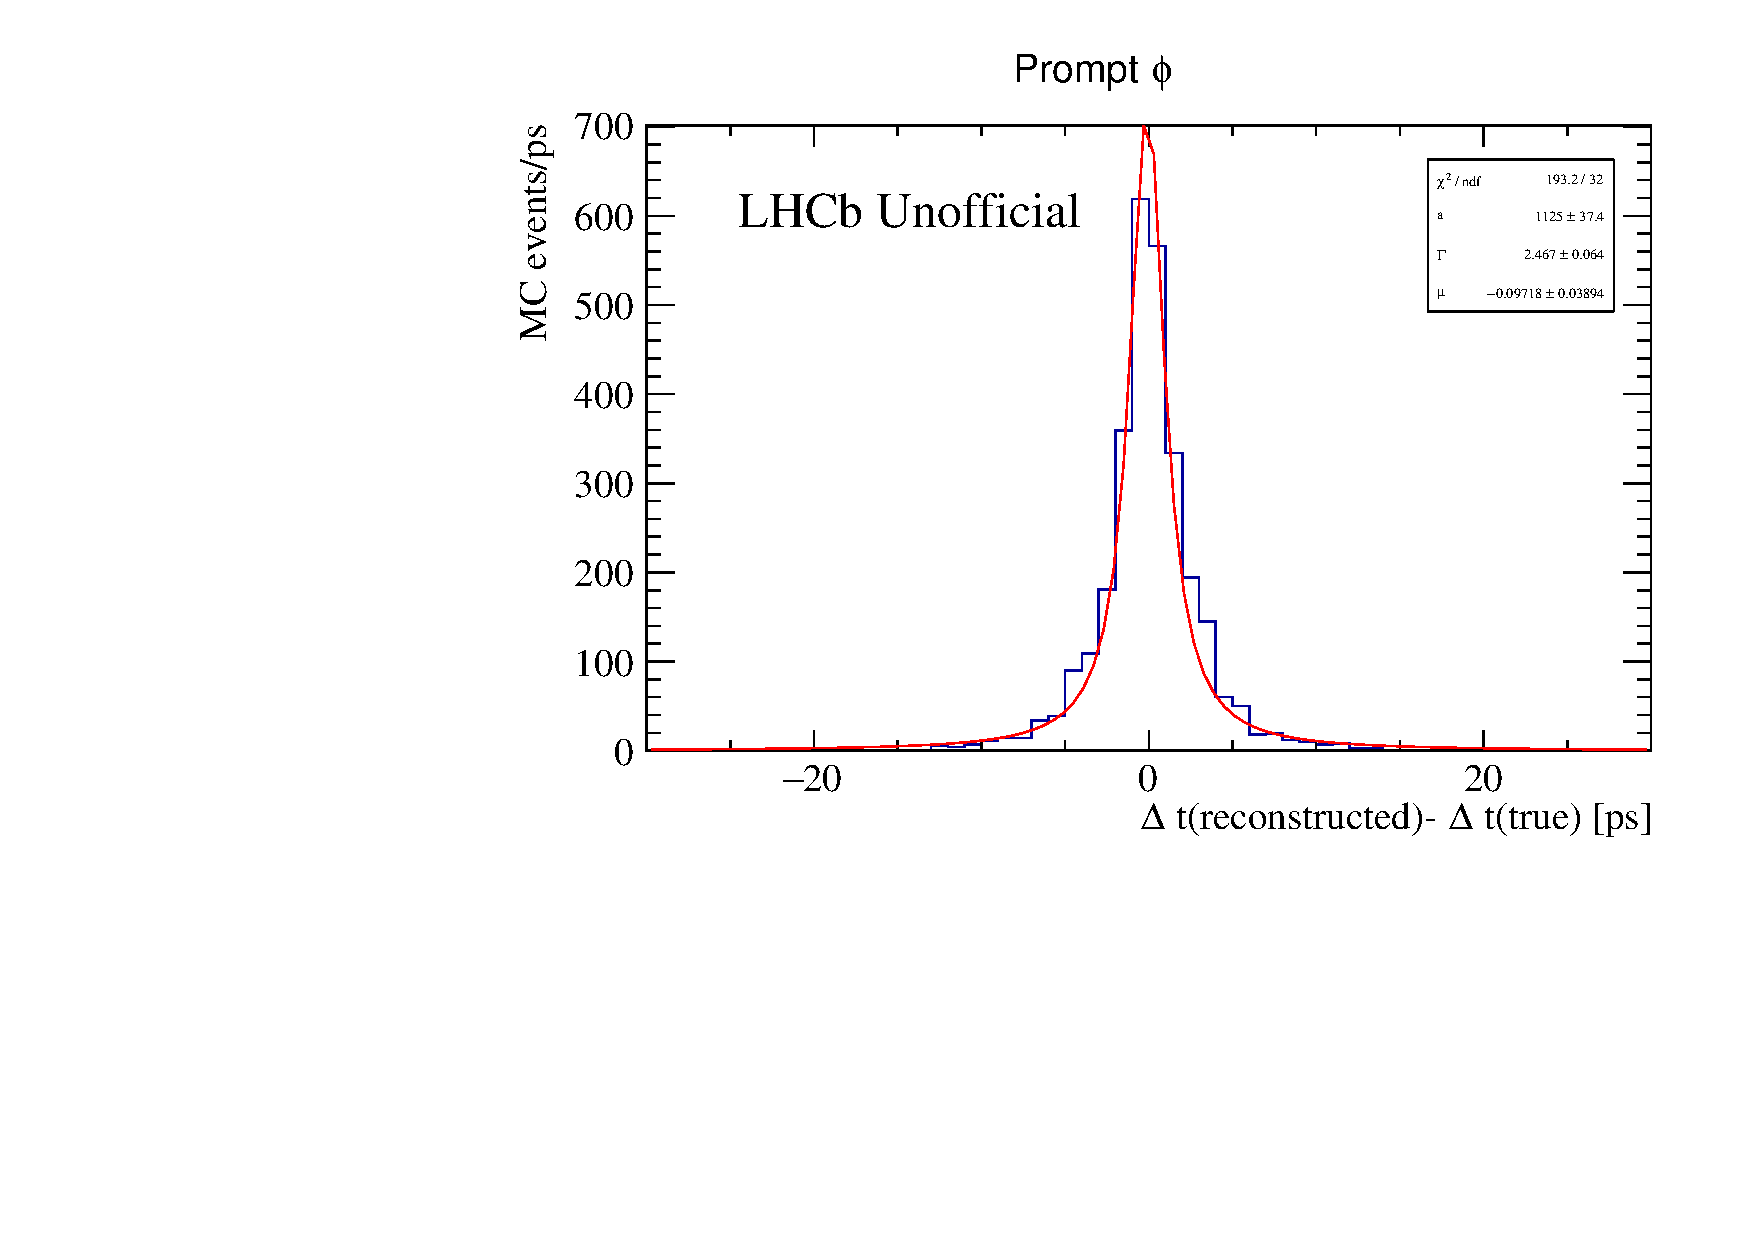
\includegraphics[width=.49\textwidth]{figs/time_res_incl/timeResolution-DeltaTauLD.pdf}
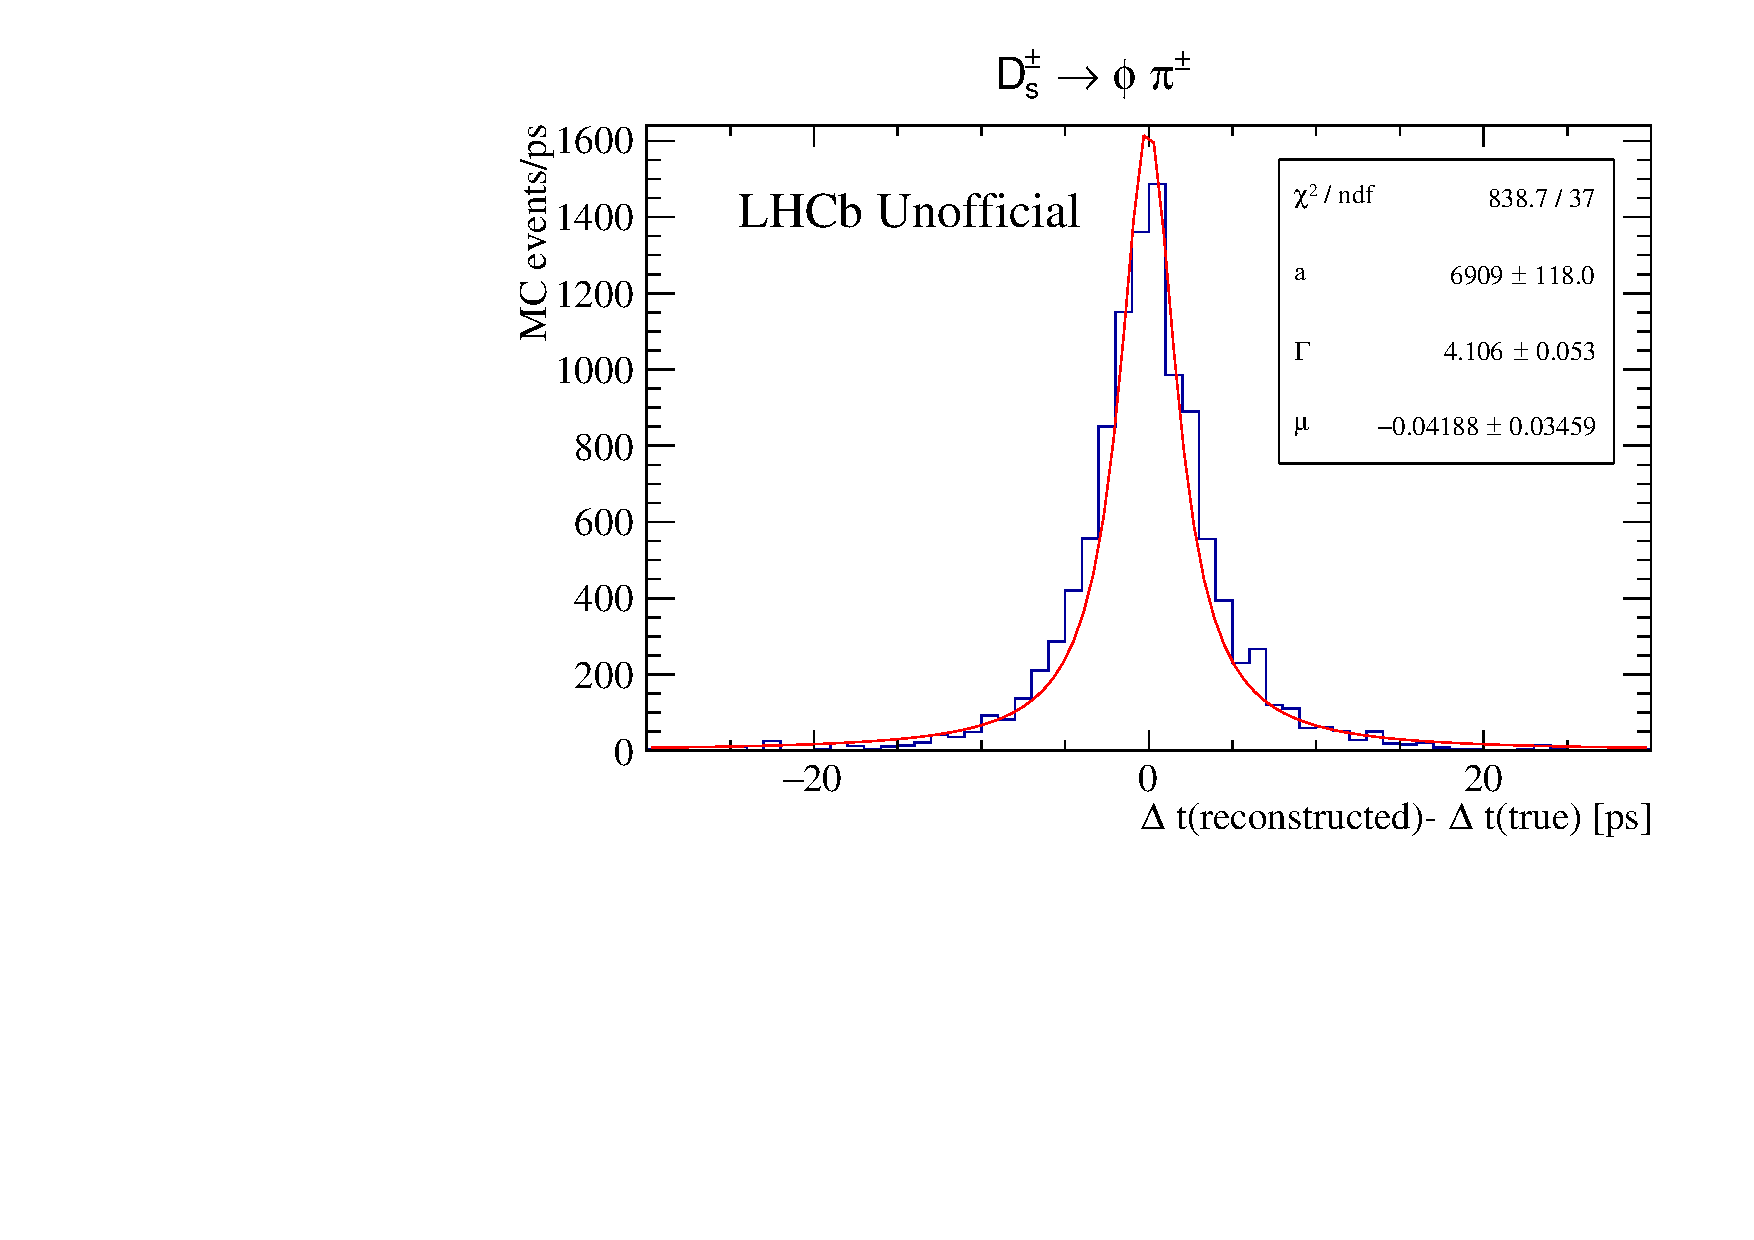
\includegraphics[width=.49\textwidth]{figs/time_res_Ds/timeResolution-DeltaTauLD.pdf}
\captionof{figure}{Resolution of $\Delta t$ for LL and DD kaons reconstructed using the TupleToolPropertime. }\label{FIG:LD-diff}
\end{center}

For the $D_s^\pm \rightarrow \phi \pi^\pm$ case, the width of the resolution of the decay time difference is smaller than for the actual decay times since the $\phi$ lifetime is negligible and therefore the residuals of the kaon decay times are correlated through the common ``vertex'' $D_s^\pm \rightarrow K^0 \overline{K}^0 \pi^\pm$ as can be seen in figure \ref{FIG:correlation}.

\begin{center}
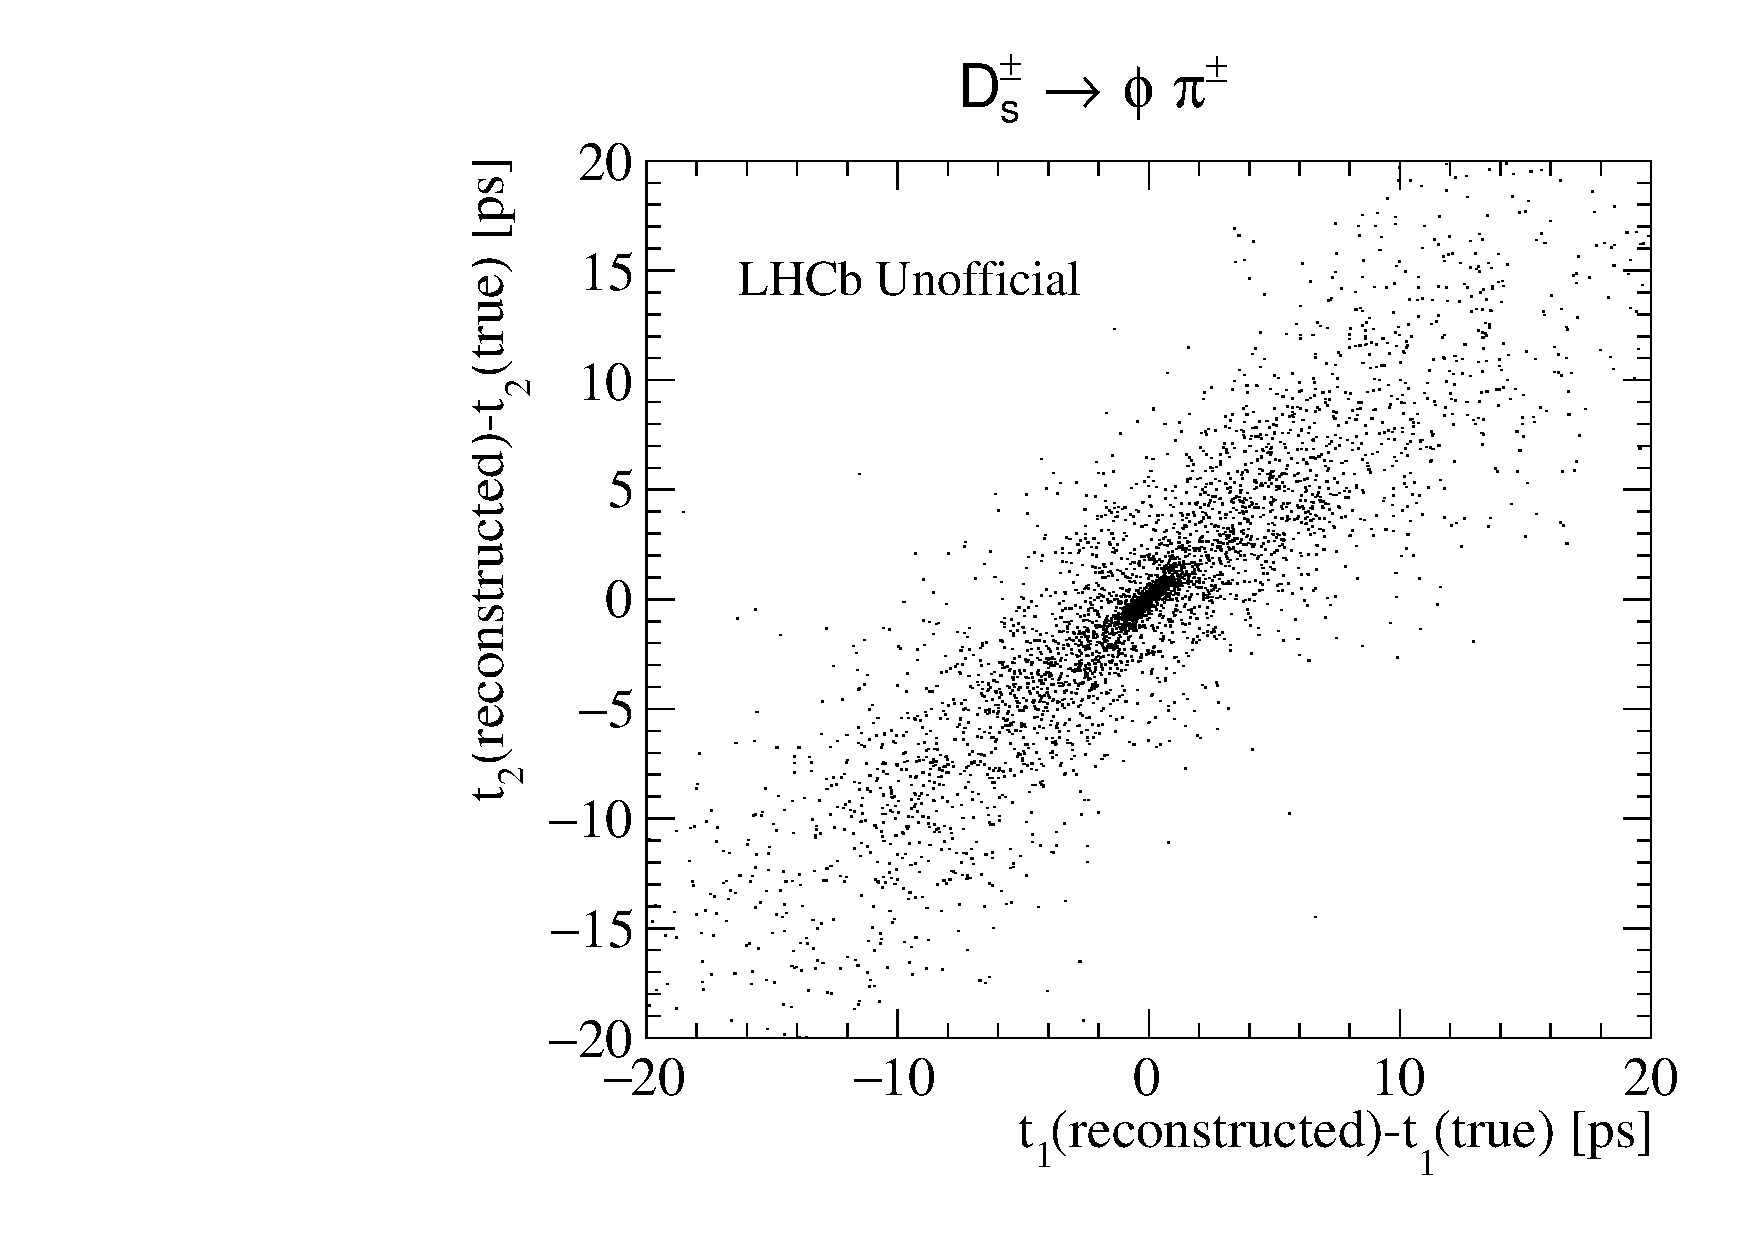
\includegraphics[width=.7\textwidth]{figs/time_res_Ds/UReco_2D.pdf}
\captionof{figure}{Correlation between the decay time residuals of both neutral kaons due to the common origin vertex.}\label{FIG:correlation}
\end{center}




\section{Toy model for the prompt $\phi$ approach}
Since the decay intensity of two prompt $K_S$ is simply 
\begin{equation}
I(t_1,t_2) \propto e^{-\Gamma_S t_1}e^{-\Gamma_S t_2}, 
\end{equation} 
a toy study based on the assumption that all background consists of prompt $K_S$ has been done using RooFit. To make the model more realistic, it includes an approximate transverse momentum distribution which is shown in figure \ref{FIG:Mommodel}. 

\begin{center}
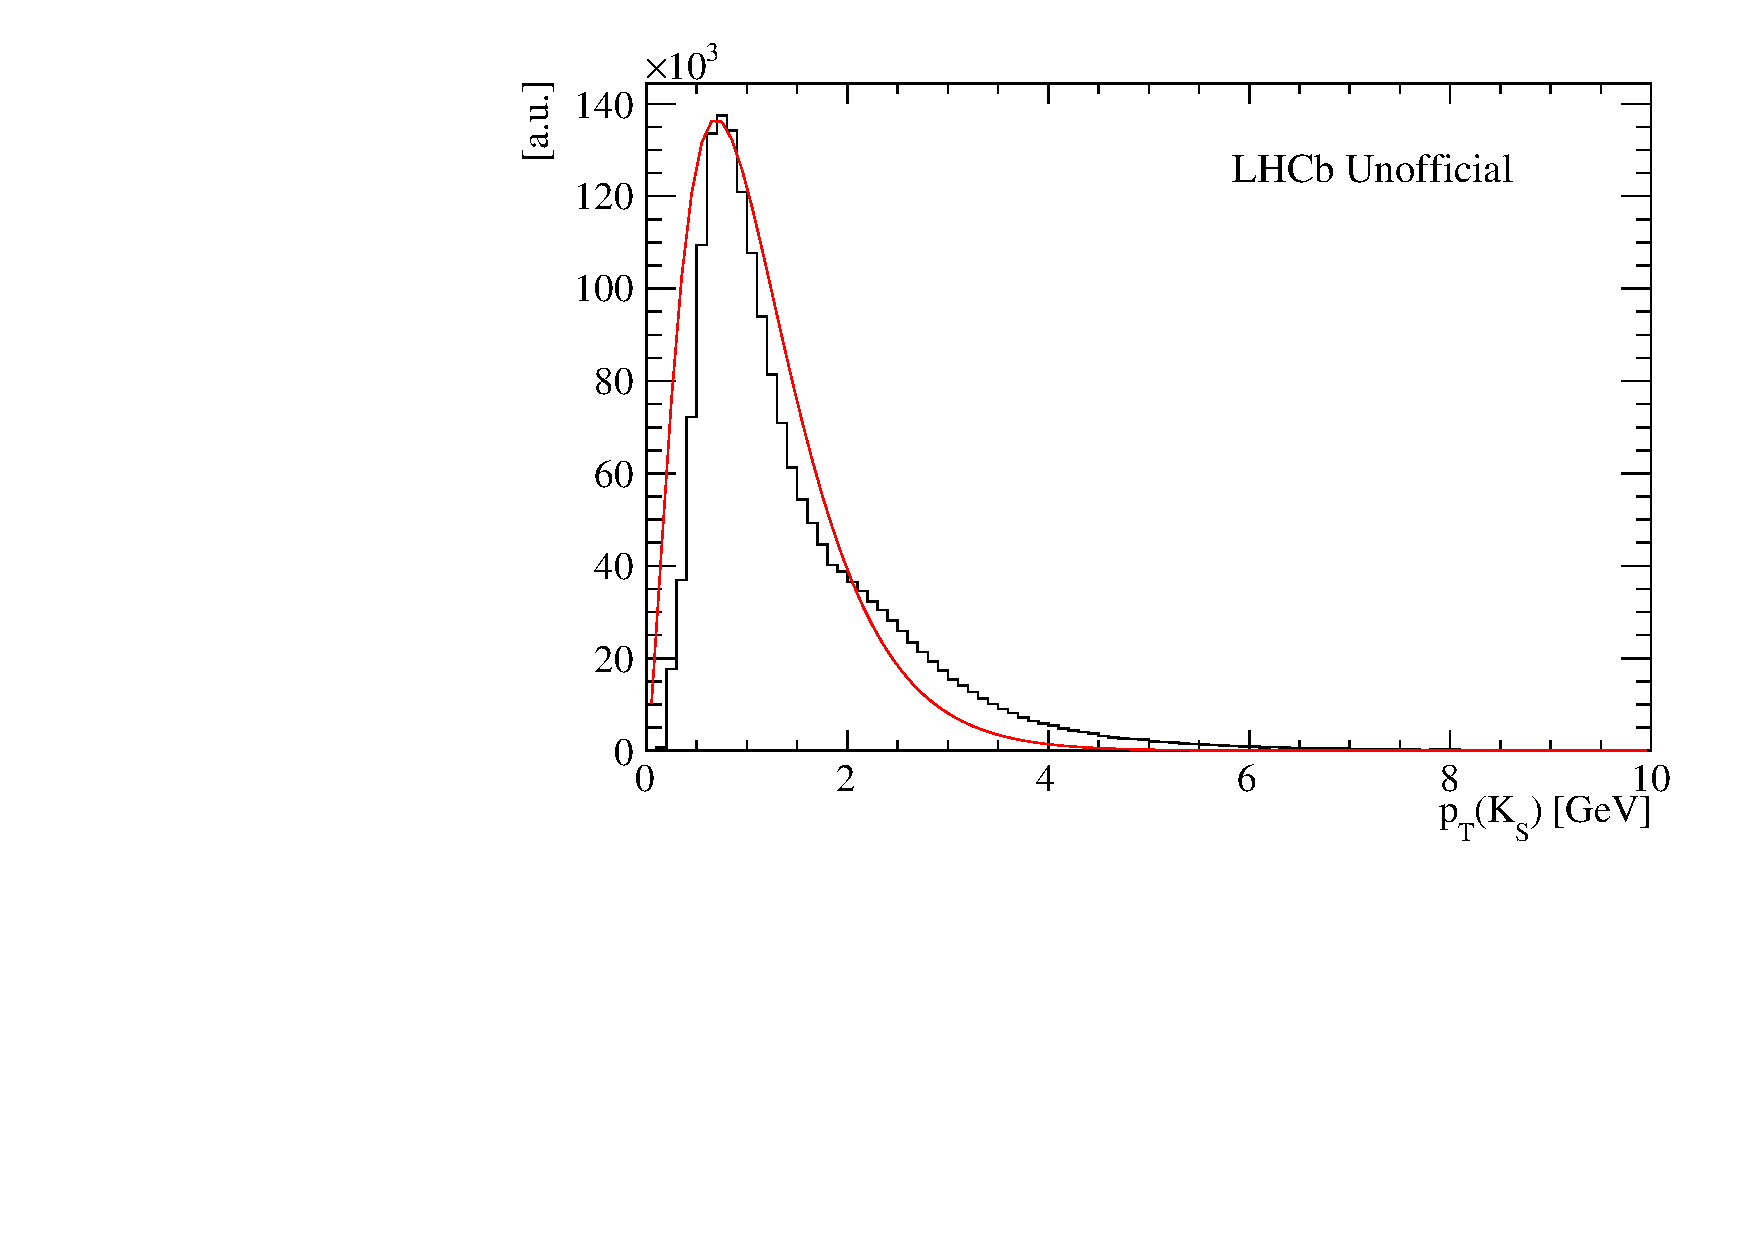
\includegraphics[height=.48\textwidth]{figs/mommodel.pdf}
\captionof{figure}{Transverse momentum of the kaons. The black line shows the distribution in 2012 data and the red line the approximation used in the model.}\label{FIG:Mommodel}
\end{center}

The approximative form used is
\begin{equation}
N(p_T(K_S)) \propto 
(p_T[MeV])^{1.52}\exp\left(-2.19\cdot10^{-3}p_T[MeV]\right) 
\end{equation}
It being part of the model is necessary in order to transfer the acceptance of events based on the transverse coordinates of the kaon decay vertices into the time domain that was studied. If for example both kaons decay inside the beampipe, that means that the $x$ and $y$ coordinate of their decay vertices have to be less than \SI{7}{mm}.

\begin{center}
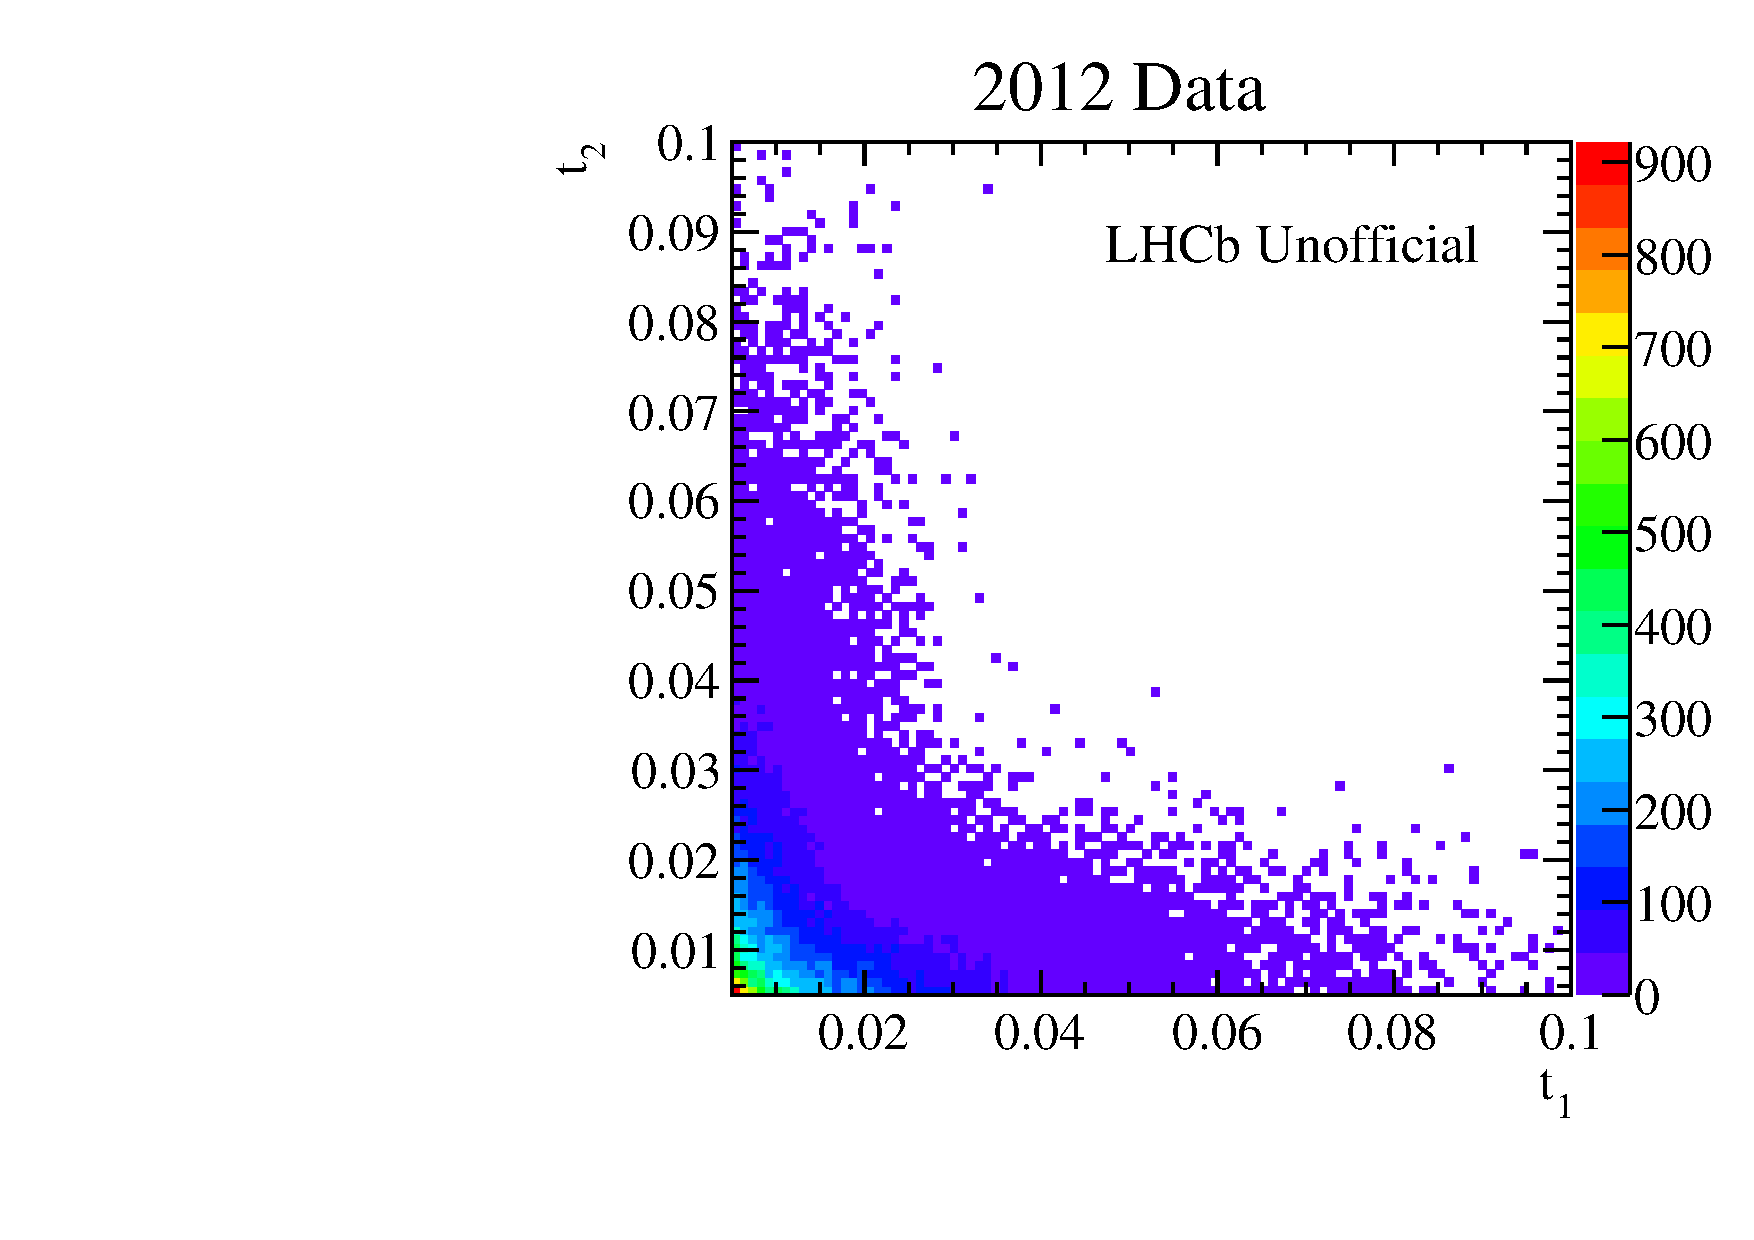
\includegraphics[width =.49\textwidth]{figs/data.pdf}
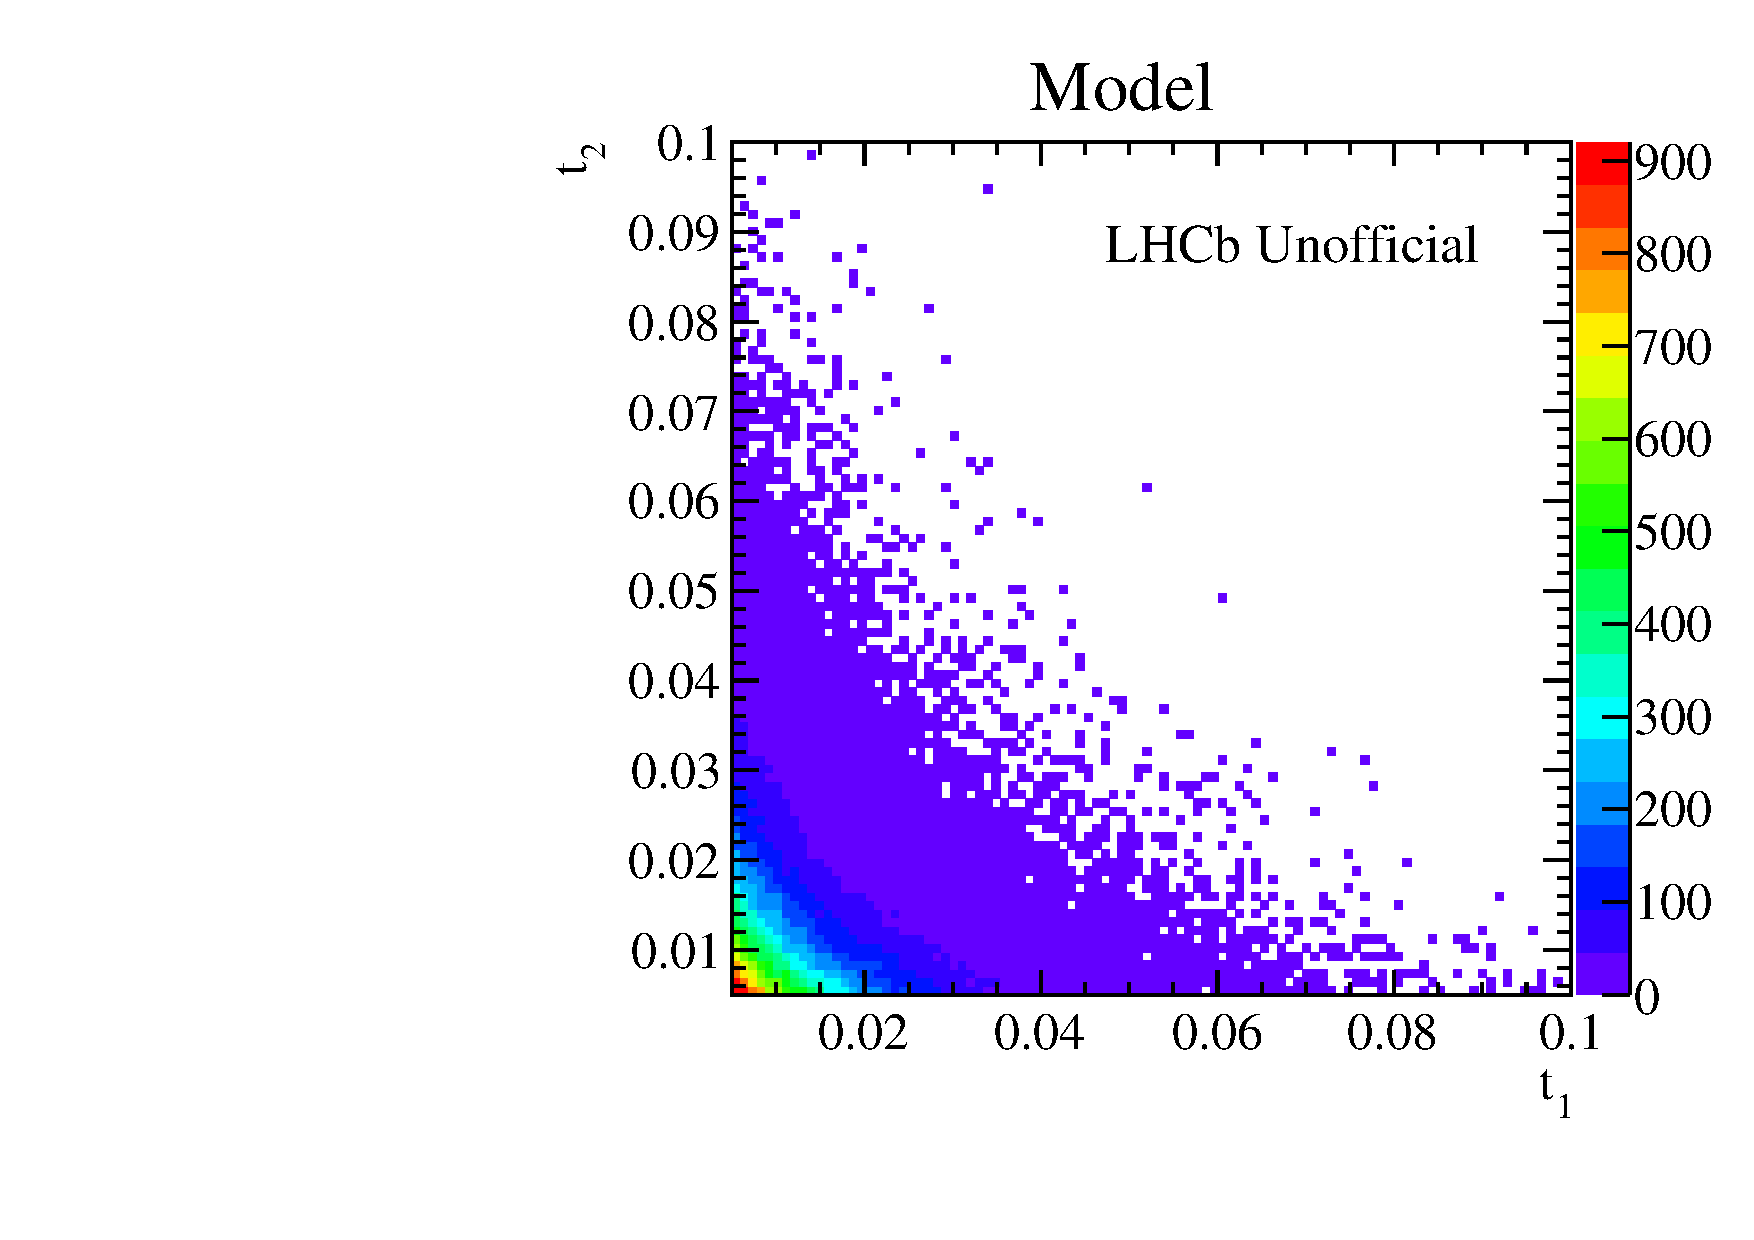
\includegraphics[width =.49\textwidth]{figs/model.pdf}
\captionof{figure}{Comparison between the distribution in the lifetimes of the two kaons for 2012 data and the toy model studied.}\label{FIG:2D}
\end{center}

The distribution of the decay times of the two kaons as given by the 2012 data and the model are displayed in figure \ref{FIG:2D}




A toy dataset was built by combining this model of the prompt $K_S$ with a similar one where the decay intensity of the kaons is replaced with the one given in equation \eqref{EQ:DI1} describing Standard Model background ($\zeta_{SL}=0$). They were added with weights according to a signal to background ratio of $4\cdot10^{-4}$. This ratio is an optimistic estimate gained from the efficiency study in section  \ref{SEC:Efficiencies}.



Afterwards, the RooStats profile likelihood calculator was used to determine a 95\% C.L. limit on $\zeta_{SL}$ for different luminosities based on this composite model. That was done by fitting equation \eqref{EQ:DI2} to the toy data set, leaving $\zeta_{SL}$ as a free parameter. The result is displayed in figure \ref{FIG:Limits}.

The predicted limits on $\zeta_{SL}$ go with the square root of the luminosity. The limits from the toy study have been fitted to a function with this behaviour. Based on this fit, it has been extrapolated that the necessary luminosity for being competitive with the KLOE limit $\zeta_{SL} = 0.098$ is $\int L\,dt \approx 275\,\text{fb}^{-1}$. This is far beyond the amount of luminosity planned to be collected during run II and run III.

\begin{center}
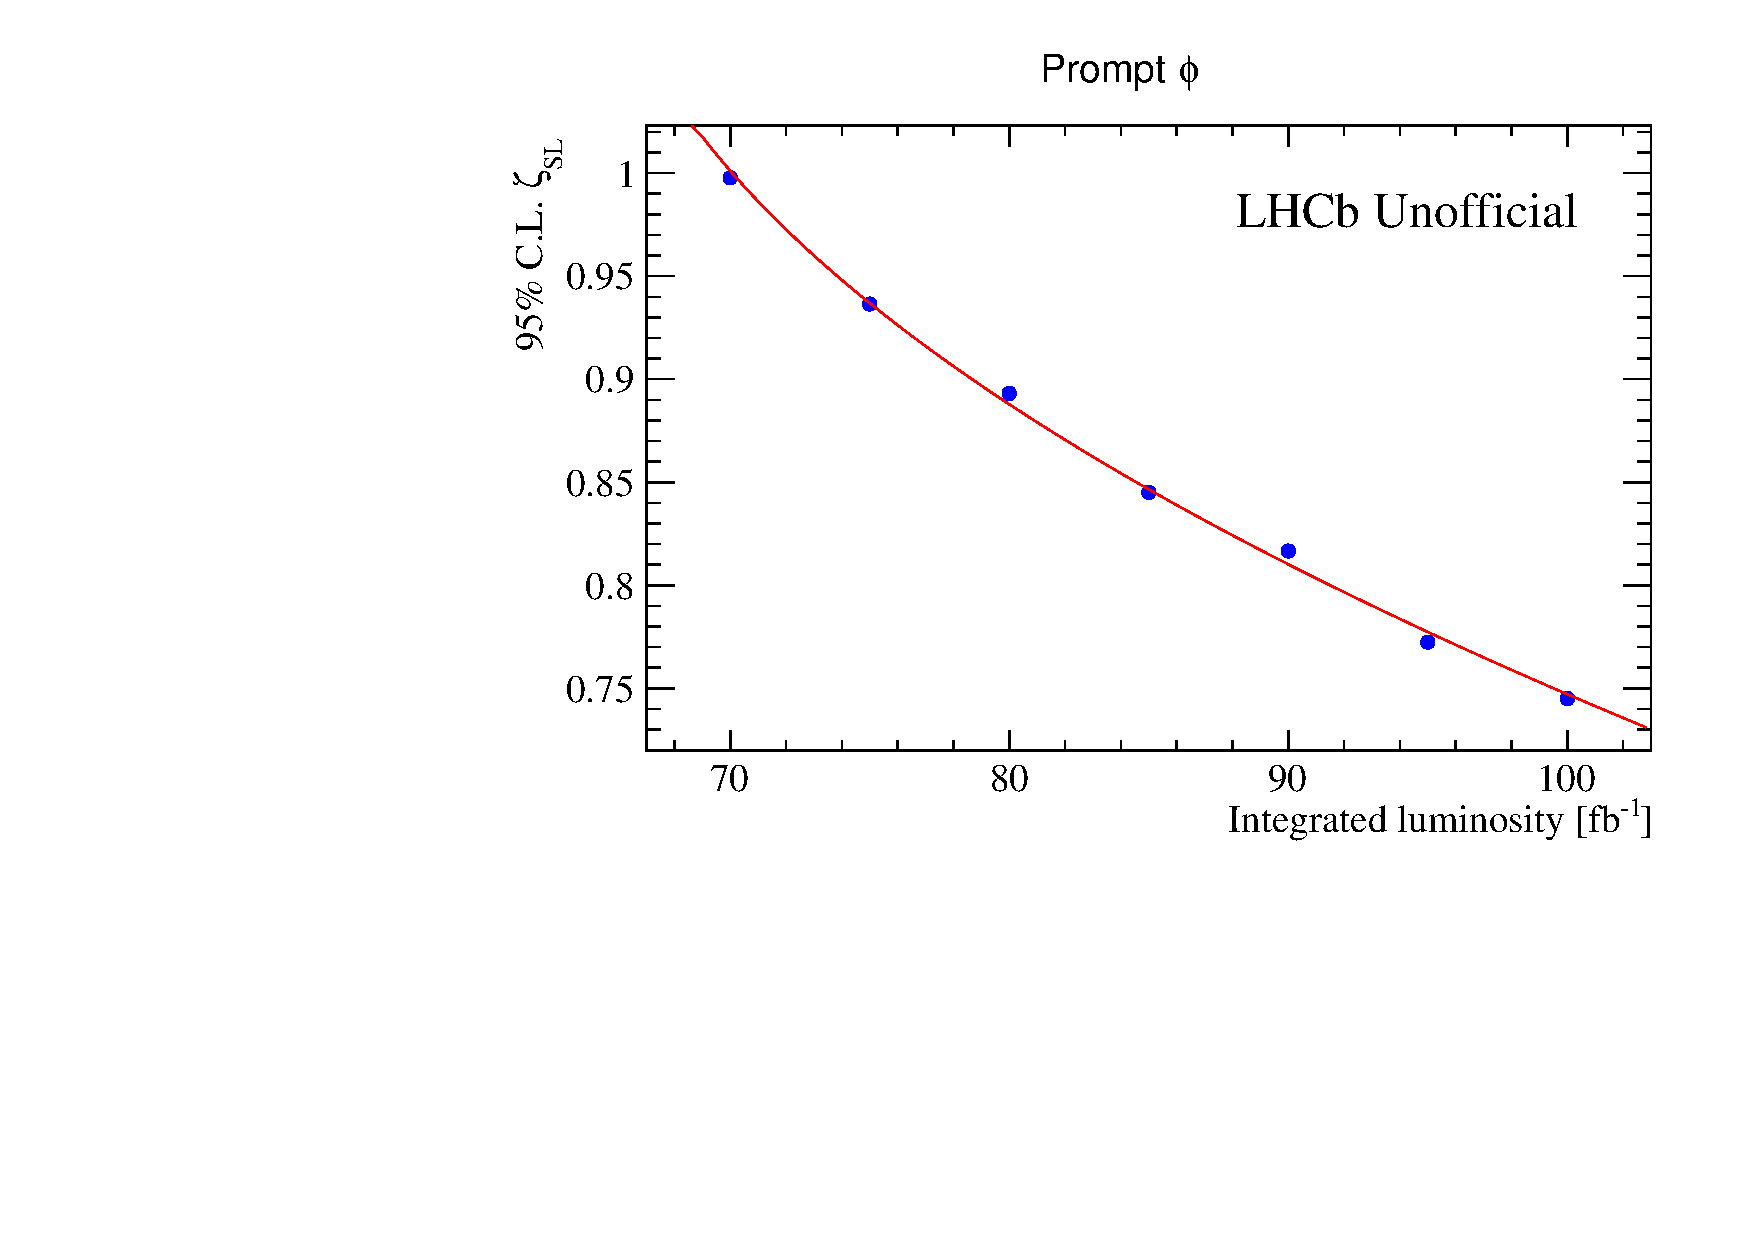
\includegraphics[width=.7\textwidth,trim= 0mm 0mm 0mm 10mm, clip]{figs/limits.pdf}
\captionof{figure}{Predicted 95\% C.L. limit on $\zeta_{SL}$ for the given luminosities.} \label{FIG:Limits}
\end{center}



%\item Fitted to 
%\begin{align*}
%I(t_1,t_2) \propto & e^{-\Gamma_L t_1 - \Gamma_S t_2} +e^{-\Gamma_S t_1 - \Gamma_L t_2}\\& - 2(1-\zeta_{SL}) e^{-\frac{1}{2}\left(\Gamma_S + \Gamma_L\right)\left(t_1+t_2\right)}\cos\left(\Delta m \left(t_1-t_2\right)\right)
%\end{align*}
%\item Derived limit on $\zeta_{SL}$ from fit result 
%\end{itemize}
%\end{frame}
\section{Conclusion}
The signal and background yields for the two approaches of $\phi$ selection have been calculated. The result suggests that the use of the topology $D_s^\pm \rightarrow \phi\pi^\pm$ does not offer significant improvement in the signal to background ratio.

The time resolution of the LHCb detector and the reconstruction algorithms commonly used by the collaboration have been studied in depth.

Finally, a toy study for the prompt $\phi$ approach has been conducted, resulting in the prediction that the luminosity needed at LHCb to reach the level of precision KLOE has for the measurement of CPT invariance in $\phi \rightarrow K^0\overline{K}^0$ is in the order of \SI{275}{fb^{-1}}.

It can be concluded that with the means currently available to LHCb, the study of CPT invariance in the given system does not seem feasible.
\section{Acknowledgments}
I would like to thank my supervisors Giulio Dujany and George Lafferty for giving me the opportunity to be a CERN summer student. Thank you for your support and counseling, it was great working with you! 
Thank you to Jonathan Harrison for providing a good part of the basis for my work and to Lorenzo Capriotti for helping me with my first steps using the Grid. 
I am very grateful to the entire LHCb group of the University of Manchester for welcoming me this summer. 





\addcontentsline{toc}{section}{References}
\setboolean{inbibliography}{true}
\bibliographystyle{LHCb}

\bibliography{citations}




\end{document}
